\documentclass[12pt]{article}
\usepackage{amssymb}
\usepackage{multicol,multienum}
\usepackage{latexsym,amssymb,amsmath}
\usepackage{indentfirst}
\usepackage{cases}
\usepackage{color}
\usepackage{graphicx}
\usepackage{mathrsfs}
\usepackage{amsthm}
\usepackage{bm}
\usepackage{CJK}
\usepackage{url}
\usepackage[font={sf,bf},textfont=md]{caption}
\usepackage{animate}
\usepackage{hyperref}
\usepackage{multirow}
\usepackage{interval}
\usepackage[table,xcdraw]{xcolor}
\usepackage{subcaption}
\usepackage{caption}
\usepackage{bm}
\usepackage{thmtools, thm-restate}
\usepackage{bbm}
\usepackage{verbatim}
\usepackage{wrapfig}
\usepackage{lscape}
\usepackage{rotating}
\usepackage{algorithm}
\usepackage{enumitem}
\usepackage{natbib}
\usepackage[noend]{algpseudocode}
\usepackage{bbding}
\usepackage{booktabs}
\usepackage{titlesec}
\usepackage{bigstrut}
\usepackage[stable]{footmisc}
\usepackage{multibib}
\newcites{online}{References}


%\pdfminorversion=4
% NOTE: To produce blinded version, replace "0" with "1" below.
\newcommand{\blind}{0}

\iffalse
% DON'T change margins - should be 1 inch all around.
\addtolength{\oddsidemargin}{-.5in}%
\addtolength{\evensidemargin}{-.5in}%
\addtolength{\textwidth}{1in}%
\addtolength{\textheight}{-.3in}%
\addtolength{\topmargin}{-.8in}%
\fi

\addtolength{\oddsidemargin}{-.6in}%
\addtolength{\evensidemargin}{-.6in}%
\addtolength{\textwidth}{1.2in}%
\addtolength{\textheight}{0.4in}%
\addtolength{\topmargin}{-0.8in}%

\newcommand{\beginsupplement}{%
        \setcounter{table}{0}
        \renewcommand{\thetable}{S\arabic{table}}%
        \setcounter{figure}{0}
        \renewcommand{\thefigure}{S\arabic{figure}}%
        \setcounter{page}{0}
     }

\newcommand{\pkg}[1]{{\fontseries{b}\selectfont #1}} 
%\newtheorem{theorem}{Theorem}[section]
\newtheorem{theorem}{Theorem}
\newtheorem{corollary}{Corollary}[theorem]
\newtheorem{lemma}{Lemma}

\newcommand{\N}{{\mathbb{N}}}  % the natural numbers
\newcommand{\Z}{{\mathbb{Z}}}  % the integers
\newcommand{\Q}{{\mathbb{Q}}} % the rational numbers
\newcommand{\R}{{\mathbb{R}}}  % the real numbers
\newcommand{\C}{{\mathbb{C}}}  % the complex numbers

\DeclareMathOperator*{\argmin}{arg\,min}
\DeclareMathOperator*{\argmax}{arg\,max}

\begin{document}

%\bibliographystyle{natbib}

\def\spacingset#1{\renewcommand{\baselinestretch}%
{#1}\small\normalsize} \spacingset{1}


%%%%%%%%%%%%%%%%%%%%%%%%%%%%%%%%%%%%%%%%%%%%%%%%%%%%%%%%%%%%%%%%%%%%%%%%%%%%%%


\if0\blind
{
  \title{\bf On the use of information criteria for subset selection in least squares regression}
  \author{Sen Tian\\
    and \\
    Clifford M. Hurvich \\
    and \\
    Jeffrey S. Simonoff \\
    Department of Technology, Operations, and Statistics, \\ Stern School of Business, New York University}
  \date{}
  \maketitle
} \fi

\if1\blind
{
  \bigskip
  \bigskip
  \bigskip
  \begin{center}
    {\LARGE\bf On the use of information criteria for subset selection in least squares regressions}
\end{center}
  \medskip
} \fi

\begin{abstract}
  Least squares (LS) based subset selection methods are popular in regression modeling. Best subset selection (BS) is known to be NP hard and has a computational cost that grows exponentially with the problem size. In this paper, we propose a novel LS based method, the best orthogonalized subset selection (BOSS) method, that 

\end{abstract}


\iffalse
\begin{abstract}
  Best subset selection (BS) is a popular least squares (LS) based subset selection method for regression modeling. In order to select the optimal subset size, one often applies an information criterion such as the Mallows' C$_p$. \citet{Ye1998} and \citet{Efron2004} demonstrated that with the effective degrees of freedom (edf) being plugged in place of the subset size, C$_p$-edf provides an unbiased estimate of the prediction error. This paper is largely motivated by the following challenges of applying BS in practice: (1) BS is NP-hard and its computational cost grows exponentially with the problem size; and (2) the edf for BS generally does not have an analytical expression. In this paper, we start from a restricted case (orthogonal design matrix $X$). We build a connection between BS and its Lagrangian version, and propose a heuristic degrees of freedom (hdf) for BS, which can be estimated via an analytically-based expression. Furthermore, we introduce AICc-edf and its feasible version AICc-hdf, which are motivated by trying to construct an unbiased estimator of the Kullback-Leibler divergence for BS. Finally, we return to a general $X$ and propose a novel LS-based method, the best orthogonalized subset selection (BOSS) method. BOSS along with AICc-hdf works well in both simulations and real data analysis, with the computational effort of a single ordinary LS fit. 
\end{abstract}
\fi


\noindent%
{\it Keywords:} Best subset regression, effective degrees of freedom, information criteria.
\vfill

\newpage
\spacingset{1.5} % DON'T change the spacing!

 %!TEX root = boss.tex
\section{INTRODUCTION}
Suppose that we have the data generating process
\begin{equation}
\mathbf{y}=\mathbf{\mu}+\mathbf{\epsilon},
\label{eq:truemodel_def}
\end{equation}
where $\mathbf{y}\in \mathcal{R}^n$ is the response vector, $\mathbf{\mu} \in \mathcal{R}^n$, is the fixed mean vector, and $\mathbf{\epsilon} \in \mathcal{R}^n$ is the noise vector. The mean vector is estimated based on a fixed design matrix $\mathbf{X}\in \mathcal{R}^{n\times p}$. We assume the error $\mathbf{\epsilon} \sim \mathcal{N}(0,\sigma^2 I)$ and $n > p$.
%\stackrel{iid} can be used to add `iid' on top of `sim'

\subsection{Best Subset Selection}
Best subset selection (BS) \citep{Hocking1967} seeks the set of predictors that best fit the data in terms of quadratic error for each given subset size (excluding the intercept) $k\in\{0,1,\cdots,p\}$, i.e. it solves the following constrained optimization problem:
\begin{equation}
\min_{\beta_0, \beta} \frac{1}{2} \lVert \mathbf{y}-\beta_0\mathtt{1} -\mathbf{X\beta}\rVert_2^2 \quad \text{subject to} \quad \lVert \mathbf{\beta} \rVert_0 \le k,
\label{eq:bestsubset-setup}
\end{equation}
where $\lVert \mathbf{\beta} \rVert_0 = \sum_{i=1}^{p} \mathtt{1}(\beta_i \ne 0)$ is the number of non-zero coefficients in $\mathbf{\beta}$. Note that to simplify the discussion, we assume that the intercept term $\beta_0=0$ throughout the paper, except in the real data examples, where all of the fitting procedures include an intercept.


% computation of BS
BS is known to be an NP-hard problem \citep{Natarajan1995} and its computational cost grows exponentially with the dimension $p$. Many attempts have been made to reduce the computational cost of the method. The most well-known approach is the branch-and-bound algorithm ``leaps" \citep{Furnival1974} that solves \eqref{eq:bestsubset-setup} in seconds for $p$ being up to around $30$. More recently, \citet{Bertsimas2016} formulated \eqref{eq:bestsubset-setup} using a mixed integer operator (MIO), and largely reduced the computing overhead by using a well-developed optimization solver such as {\tt GUROBI} or {\tt CPLEX}. However, according to \citet{Hastie2017}, MIO normally takes about $3$ minutes to find the solution at a given size $k$ for a problem with $n=500$ and $p=100$. The current methodology is not scalable to very large datasets, and solving \eqref{eq:bestsubset-setup} remains a challenge for most real world applications.

% edf of BS
In order to select the optimal tuning parameter, e.g. the subset size $k$ in \eqref{eq:bestsubset-setup}, one often applies an information criterion, which augments the training error with the effective degrees of freedom (edf). \citet{Efron1986} defined the edf for a general fitting rule $\hat{\mu}$ as:
\begin{equation}
\text{edf}(\hat{\mu}) = \frac{1}{\sigma^2} \sum_{i=1}^{n} \text{cov}(\hat{\mu}_i,y_i).
\label{eq:edf}
\end{equation}
It is easy to verify that edf for the linear regression of $y$ upon $X$ is the number of estimated coefficients $p$. However, \citet{janson2015effective} showed in simulations that there can be a large discrepancy between the edf of BS at size $k$ and $k$ itself. Similar evidence can be found in \citet{Tibshirani2015}, where the author quantifies the difference as the search degrees of freedom, which accommodates the amount of searching that BS performs in order to choose a best $k$-predictor subset. Unfortunately, the edf of BS does not have an analytical expression except when $X$ is orthogonal and $\mu=0$ \citep{Ye1998}. Numerically, we can apply tools like data perturbation \citep{Ye1998}, bootstrap \citep{Efron2004} or data randomization \citep{Harris2016} to estimate edf, but all rely on tunings of some hyperparameters and can be computationally intensive. 

This paper is motivated by the above challenges. We propose a heuristic degrees of freedom (hdf) for BS by assuming an orthogonal $X$. We further introduce a novel least squares (LS) based subset selection method, the best orthogonalized subset selection (BOSS), and we demonstrate that BOSS using an information criterion with hdf works well in practice for a general $X$ with the computational cost of a single ordinary LS fit.

\subsection{Optimism Theorem and Information Criteria for BS}
\label{sec:optimism}
Information criteria are designed to provide an unbiased estimate of the prediction (or testing) error, and can be derived from the so-called optimism theorem. Denote $\Theta$ as an error measure, $\text{err}$ as the training error, $\text{Err}$ as the testing error, $y^0$ as a new response vector with the same distribution but independent of the original $y$, and $E_0$ is the expectation taken over $y^0$. \citet{Efron1986} defined the optimism as 
\begin{equation*}
\text{op} = \text{Err} - \text{err},
%\label{eq:op}
\end{equation*}
and introduced the optimism theorem,
\begin{equation*}
E(\text{op}) = E(\text{Err}) - E(\text{err}).
%\label{eq:op_thm}
\end{equation*}
A straightforward result from the optimism theorem is that 
\begin{equation}
\widehat{\text{Err}} = \text{err} + E(\text{op})
\label{eq:err_eop}
\end{equation}
is an unbiased estimator of $E(\text{Err})$, and is intended to balance the trade-off between model fit and model complexity. The challenge is to find $E(\text{op})$ for a given fitting rule $\hat{\mu}$ and error measure $\Theta(y,\hat{\mu})$.

When the error measure $\Theta$ is the squared error (SE), i.e. $\Theta(y_i,\hat{\mu}_i)=(y_i-\hat{\mu}_i)^2$, $\text{err}_{\text{SE}}$ (denoted as the training error when $\Theta$ is SE) then becomes the residual sum of squares $\text{RSS} = \sum_{i=1}^{n} \Theta(y_i, \hat{\mu}_i)$, and the testing error $\text{Err}_\text{SE} =\sum_{i=1}^n E_0[\Theta(y^0_i,\hat{\mu}_i)]$. \citet{Ye1998} and \citet{Efron2004} proved that for a general fitting rule $\hat{\mu}$ such as BS, $E(\text{op}_{\text{SE}})=2\sigma^2 \cdot \text{edf}(\hat{\mu})$, and hence $\widehat{\text{Err}}_{\text{SE}}$ in \eqref{eq:err_eop} becomes C$_p$-edf where 
\begin{equation}
\text{C}_p\text{-edf} = \text{RSS} + 2 \sigma^2 \cdot \text{edf}.
\label{eq:cp_edf}
\end{equation}
These authors also showed that the traditional C$_p$,
\begin{equation*}
\text{C}_p\text{-ndf} = \text{RSS} + 2 \sigma^2 \cdot \text{ndf},
%\label{eq:cp_ndf}
\end{equation*}
can be greatly biased when applied for BS, since C$_p$-ndf \citep{mallows1973some} was derived for a linear estimation rule $\hat{\mu} = Hy$ where $H$ is independent of $y$, which is not the case for BS. Here ndf denotes the naive degrees of freedom, i.e. $\text{Tr}(H)$. A further major issue regarding applying C$_p$ in practice is that it requires an estimate of $\sigma^2$. 

Another commonly used error measure is the deviance (up to a constant)
\begin{equation}
\Theta = -2 \log f(y|\mu,\sigma^2),
\label{eq:deviance_def}
\end{equation}
where $f$ is a pre-specified parametric model. Let $\hat{\mu}$ and $\hat{\sigma}^2$ be the maximum likelihood estimators obtained by maximizing $f(y|\mu,\sigma^2)$. We then have $\text{err}_{\text{KL}} = -2 \log f (y|\hat{\mu},\hat{\sigma}^2)$ and $\text{Err}_{\text{KL}}  = -2 E_0 \left[ \log f(y^0|\hat{\mu},\hat{\sigma}^2)\right] $, where the latter is the Kullback-Leibler (KL) discrepancy. For a linear estimation procedure, assuming asymptotic normality of $\hat{\mu}$ and $\hat{\sigma}^2$ ($f$ not necessarily Gaussian) and the true model distribution being contained in the specified parametric model $f$, \citet{konishi2008information} proved that $E(\text{op}_{\text{KL}}) = 2 \cdot \text{ndf} + o(1)$, and AIC \citep{Akaike1973},
\begin{equation*}
-2 \log f (y|\hat{\mu},\hat{\sigma}^2) + 2 \cdot \text{ndf},
\end{equation*}
asymptotically equals $\widehat{\text{Err}}_\text{KL}$ \eqref{eq:err_eop}. If $f$ follows a Gaussian distribution, as assumed in \eqref{eq:truemodel_def}, AIC can be expressed as
\begin{equation*}
\text{AIC-ndf} = n \log\left(\frac{\text{RSS}}{n}\right) + 2 \cdot \text{ndf}.
%\label{eq:aic_ndf}
\end{equation*}
\citet{Hurvich1989} replaced the asymptotic $E(\text{op}_\text{KL})$ with its exact value, for Gaussian linear regression with an assumption that the predictors with non-zero true coefficients are included in the model, and used the corrected AIC
\begin{equation*}
\text{AICc-ndf} = n \log\left(\frac{\text{RSS}}{n}\right) + n \frac{n+\text{ndf}}{n-\text{ndf}-2}.
\label{eq:aicc_ndf}
\end{equation*}
Neither AIC nor AICc has a penalty term depending upon $\sigma^2$, a clear advantage over C$_p$.

It remains a challenge to derive a KL-based information criterion for BS. \citet{Liao2018} estimated $E(\text{op}_{\text{KL}})$ via Monte Carlo simulations, but this relies on thousands of fits of the procedure, which is not computationally feasible for large datasets. 

In this work, we propose AICc-edf
\begin{equation}
\text{AICc-edf} = n \log\left(\frac{\text{RSS}}{n}\right) + n \frac{n+\text{edf}}{n-\text{edf}-2}
\label{eq:aicc_edf}
\end{equation}
for this purpose. We demonstrate that $E(\text{AICc-edf})$ approximates $E(\text{Err}_\text{KL})$ well for BS. Moreover, both AICc-edf and $\widehat{\text{Err}}_\text{KL}$ generally choose the same subset when used as selection rules. Furthermore, the feasible implementation AICc-hdf works reasonably well as a selection rule for BS with an orthogonal $X$ and for our proposed method BOSS with a general $X$. 

\subsection{The Structure and Contributions of this Paper}
The rest of the paper is organized as follows. In Section \ref{sec:aicc_hdf}, by assuming an orthogonal $X$, we introduce the hdf for BS. We provide a theoretical justification in a restricted scenario, and numerical justifications in general situations. We provide numerical evidence that $E(\text{AICc-edf})$ approximates $E(\text{Err}_\text{KL})$ well, and the feasible version AICc-hdf works well as a selection rule for BS. We further compare the performance of BS with that of regularization methods using feasible selection rules via simulations. In Section \ref{sec:boss}, we consider a general $X$ and propose the method BOSS. We provide numerical evidence that AICc-hdf is a reasonable selection rule for BOSS. Furthermore, we compare the performance of BOSS with that of forward stepwise regression (FS) and regularization methods in simulations. Lastly, we study some real data examples in Section \ref{sec:real_data}, and provide conclusions and potential future works in Section \ref{sec:conclusion}.

Below is guidance for applying LS-based methods in practice for data analysts.
\begin{itemize}
	\item Using information criteria in a naive way by plugging in the subset size as the degrees of freedom can lead to significantly worse performance than using edf and the feasible hdf.
	\item AICc is a better selection rule in terms of predictive performance in comparison to C$_p$, and the advantage is particularly strong when $p$ is close to $n$.
	\item AICc is not only more computationally efficient than cross-validation (CV), but also can result in subsets with better predictive performance especially when the signal-to-noise ratio (SNR) is high or the sample size $n$ is large. The SNR is defined as $\text{Var}(x^T \beta) / \sigma^2$.
	\item BOSS-AICc is generally the best LS-based method in comparison to BS and forward stepwise (FS) \citep{efroymson1960multiple} using CV as the selection rule, in terms of both computational efficiency and predictive performance.
	\item Compared to regularization methods, BOSS-AICc performs the best when SNR is high or the sample size $n$ is large. In terms of support recovery in a sparse true model, BOSS recovers the true predictors and rarely includes any false positives when SNR is high or the sample size $n$ is large. In contrast, regularization methods generally overfit. 
\end{itemize}

We make the code to reproduce the results in this paper publicly available at \url{https://github.com/sentian/BOSSreg}, as well as an R package \pkg{BOSSreg} (at the time of submission of this paper, we have submitted the R package to \textit{CRAN}.), publicly available at \url{https://github.com/sentian/BOSSreg}. 

%!TEX root = boss.tex
\section{AICc-hdf for BS with orthogonal \texorpdfstring{$X$}{Lg}}
\label{sec:aicc_hdf}
\subsection{A heuristic degrees of freedom for BS}
The edf of BS has an analytical expression only when the true model is $\mu=0$ \citep{Ye1998}. \citet{Tibshirani2015} studied the Lagrangian formulation of BS (LBS) and provided an analytical expression for edf without any restrictions on $\mu$. To distinguish between the two methods, we use df$_C(k)$ and df$_L(\lambda)$ to denote edf of BS for subset size $k$ and edf of LBS for tuning parameter $\lambda$, respectively. In this section, we introduce a heuristic degrees of freedom (hdf) for BS that is built upon the connection between df$_C(k)$ and df$_L(\lambda)$.

\subsubsection{Lagrangian BS and its edf}
For each regularization parameter $\lambda \ge 0$, LBS solves
\begin{equation}
	\min_\beta \frac{1}{2} \lVert \mathbf{y}-\mathbf{X\beta}\rVert_2^2 + \lambda\lVert \mathbf{\beta} \rVert_0.
\label{eq:lbestsubset-setup}
\end{equation} 
Both LBS \eqref{eq:lbestsubset-setup} and BS \eqref{eq:bestsubset-setup} are LS regressions of $y$ upon a certain subset of $X$. With orthogonal $X$, both problems have analytical solutions: $\hat{\beta}_i(\lambda)=z_i \mathbbm{1}_{(|z_{i}| \ge \sqrt{2\lambda})}$ for \eqref{eq:lbestsubset-setup} and $\hat{\beta}_i(k)=z_i \mathbbm{1}_{(|z_{i}| \ge |z_{(k)}|)}$ for \eqref{eq:bestsubset-setup}, where $z=X^T y$ and $z_{(k)}$ is the $k$-th largest coefficient in absolute value. These two problems are not equivalent, and there is no clear one-to-one correspondence between $\lambda$ in \eqref{eq:lbestsubset-setup} and $k$ in \eqref{eq:bestsubset-setup}. Indeed, for each $\lambda$ there exists a $k$ such that $\hat{\beta}(\lambda) = \hat{\beta}(k)$ where $\hat{\beta}(\lambda)$ is the solution of \eqref{eq:lbestsubset-setup} at $\lambda$ and $\hat{\beta}(k)$ is the solution of \eqref{eq:bestsubset-setup} at $k$, but the reverse does not necessarily hold, since there will be multiple $\lambda$ corresponding to the same solution $\hat{\beta}(k)$. Moreover, with a general $X$, solving \eqref{eq:lbestsubset-setup} does not guarantee recovery of the entire solution path given by solving \eqref{eq:bestsubset-setup} for $k=0,\dots,p$.

By assuming an orthogonal $X$, \citet{Tibshirani2015} derived an expression for df$_L(\lambda)$ based on definition \eqref{eq:edf},
\begin{equation}
\text{df}_L(\lambda) = E(k_L(\lambda)) + \frac{\sqrt{2\lambda}}{\sigma} \sum_{i=1}^{p} \left[\phi\left(\frac{\sqrt{2\lambda}-(X^T \mu)_i}{\sigma}\right) + \phi\left(\frac{-\sqrt{2\lambda}-(X^T \mu)_i}{\sigma}\right) \right],
\label{eq:thdf_expression}
\end{equation}
where the expected subset size is given as
\begin{equation}
E(k_L(\lambda)) = \sum_{i=1}^{p} \left[1-\Phi\left(\frac{\sqrt{2\lambda}-(X^T \mu)_i}{\sigma}\right) + \Phi\left(\frac{-\sqrt{2\lambda}-(X^T \mu)_i}{\sigma}\right) \right].
\label{eq:thdf_size_expression}
\end{equation}

\subsubsection{hdf for BS}
Given the similarity of problems \eqref{eq:bestsubset-setup} and \eqref{eq:lbestsubset-setup}, we would like to approximate df$_C(k)$ with df$_L(\lambda)$. One implementation of this proceeds as follows. Note that df$_C(k)$ is a discrete function of $k=0,\cdots,p$ while df$_L(\lambda)$ is a continuous function of a real variable $\lambda\ge 0$. We propose an hdf that uses $\text{df}_L(\lambda)$ for a particular value of $\lambda$ depending on $k$ as a proxy for $\text{df}_C(k)$. Based on \eqref{eq:thdf_size_expression}, $\lambda$ and $E(k_L(\lambda))$ have a clear one-to-one correspondence, which implies that we can find a unique $\lambda_k^\star$ such that $E(k_L(\lambda_k^\star)) = k$ for each $k=1,\cdots,p$. The value of hdf is df$_L(\lambda_k^\star)$ obtained by substituting $\lambda^\star_k$ into \eqref{eq:thdf_expression}. We also let hdf$(0)=0$ since df$_C(0)=0$. The implementation process is summarized in Algorithm \ref{alg:hdf}. Note that hdf requires estimates of $\mu$ and $\sigma$, and we use the estimates from the LS regression on all predictors. 

% algorithm of hdf
\begin{algorithm}
	\caption{The heuristic df (hdf) of BS for size $k$}\label{alg:hdf}
	Input: $X$ (orthogonal), $\sigma$ and $\mu$. For a given subset size $k$, 
	\begin{enumerate}[label=\arabic*.]
		\item Based on \eqref{eq:thdf_size_expression}, calculate $\lambda_k^\star$ such that $E(k_L(\lambda_k^\star)) = k$.
		\item Based on \eqref{eq:thdf_expression}, calculate hdf$(k) = \text{df}_L(\lambda_k^\star)$.
	\end{enumerate}
	Repeat the above steps for $k=1,\cdots,p$ and let hdf$(0)=0$, yielding hdf for each subset. 
	
	In place of $\mu$ and $\sigma$ in \eqref{eq:thdf_expression} and \eqref{eq:thdf_size_expression}, we use OLS estimates based on the full model, i.e. $\hat{\mu}=XX^T y$, $\hat{\sigma}^2 = \lVert y-\hat{\mu} \rVert_2^2/(n-p)$.
\end{algorithm}

\subsubsection{Theoretical justification of hdf under a null true model}
Assume $\mu=0$, with $X$ still being orthogonal. In such a restricted scenario, df$_C(k)$ has an analytical expression, which allows us to provide some theoretical justification for hdf$(k)$. We start by introducing notation, and present the main result in Theorem \ref{thm:hdf_ydf_representation} and its Corollary. The detailed proofs are given in the Supplemental Material.

Denote $\tilde{X}_{(i)}$ as the $i$-th largest order statistic in an i.i.d sample of size $p$ from a $\chi^2_1$ distribution. \citet{Ye1998} showed that
\begin{equation*}
\text{df}_C(k) = E\left( \sum_{i=1}^{k} \tilde{X}_{(i)} \right).
\end{equation*}
Let $\tilde{H}(s) = -\tilde{Q}(1-s)$ where $\tilde{Q}$ is the quantile function of a $\chi_1^2$ distribution, and $s\in (0,1)$. For $0\le s \le t \le 1$, the truncated variance function is defined as
\begin{equation*}
\tilde{\sigma}^2(s,t) = \int_{s}^{t} \int_{s}^{t} (u \wedge v -uv) d \tilde{H}(u) d \tilde{H}(v),
\end{equation*}
where $u \wedge v =\min(u,v)$. Denote $\tilde{Y}_p = \tilde{\sigma}_p^{-1}(\sum_{i=1}^k \tilde{X}_{(i)} - \tilde{\mu}_p)$, where
\begin{equation*}
\tilde{\sigma}_p = \sqrt{p} \cdot \tilde{\sigma}(1/p,k/p),
\end{equation*}
and
\begin{equation*}
\tilde{\mu}_p = -p \int_{1/p}^{k/p} \tilde{H}(u) du - \tilde{H}\left(\frac{1}{p}\right).
\end{equation*}

\begin{restatable}{theorem}{dfasy}
	\label{thm:hdf_ydf_representation}
	Assume $X$ is orthogonal and the true model is null ($\mu=0$). As $p\rightarrow  \infty$,  $k\rightarrow  \infty$ with $k=\left \lfloor{px}\right \rfloor$, we have
	\begin{equation}
	\label{eq:hdf_ydf_yp_representation}
	\frac{1}{2p} \text{hdf}(k) = \frac{1}{2p}\text{df}_C(k) - \frac{\tilde{\sigma}_p}{2p}E(\tilde{Y}_p) + O\left(\frac{\log(p)}{p} \right),
	\end{equation}
	where $x \in (0,1)$ is a constant and $\left \lfloor{\cdot}\right \rfloor$ denotes the greatest integer function.
\end{restatable}

\begin{restatable}{corollary}{dfasycorollary}
	\label{thm:hdf_ydf_corollary}
	If $\limsup |E(\tilde{Y}_p)| < \infty$ , we further have
	\begin{equation}
	\label{eq:main_corollary}
	\frac{\text{df}_C(k)}{\text{hdf}(k)} \rightarrow 1.
	\end{equation}
\end{restatable}
\noindent\textbf{Remark:} If $\tilde{Y}_p$ is uniformly integrable, then $E(\tilde{Y}_p) \rightarrow 0$, and hence the result of Corollary \ref{thm:hdf_ydf_corollary} holds.

It can be seen that Corollary \ref{thm:hdf_ydf_corollary} holds given the assumptions, since both hdf$(k)$ and df$_C(k)$ diverge while $E(\tilde{Y}_p)$ and the remainder term remain bounded. The Corollary suggests that for large $k$ and large $p$, the ratio of df$_C(k)$ to hdf$(k)$ will be close to $1$. We next explore empirically the relative behavior of the two dfs for a fixed $p$ with an increasing $k$. 

\subsubsection{Numerical justification of hdf}
Figure \ref{fig:dfc_dflambda} shows the comparison of hdf and edf via simulations. We fit BS on $1000$ realizations of the response generated after fixing $X$. The edf is calculated based on definition \eqref{eq:edf} using the sample covariances, while hdf is given by Algorithm \ref{alg:hdf}. We see that in the null case, using hdf to approximate edf becomes more accurate as $k$ approaches $p$, providing a finite-sample justification of Corollary \ref{thm:hdf_ydf_corollary}. 

In addition to the null model, we consider a sparse model (Orth-Sparse-Ex1) with $p_0=6$ true predictors (those with non-zero coefficients), and a dense model (Orth-Dense) where all predictors have non-zero coefficients. We also consider two signal-to-noise (SNR) ratios with `hsnr' and `lsnr' representing high and low SNR respectively, and the SNR is defined as $\text{Var}(x^T \beta)/\sigma^2$. The details of the setups for Orth-Sparse-Ex1 and Orth-Dense models can be found in Section \ref{sec:simulation_setup_orthx}. Similarly to the null case, we see that hdf approaches edf as $k$ gets close to $p$, i.e. the statement of Corollary \ref{thm:hdf_ydf_corollary} holds in these scenarios as well. Furthermore, we see that hdf generally approximates edf well, where the difference is more pronounced when BS underfits, e.g. a sparse model with high SNR and $k<p_0=6$ or a dense model with high SNR with $k<p=14$. Clearly, underfitting causes the problem, particularly when what is left out is important, such as in a high SNR case.   


% \ref{fig:dfc_dflambda}
\begin{figure}[!ht]
	\centering
	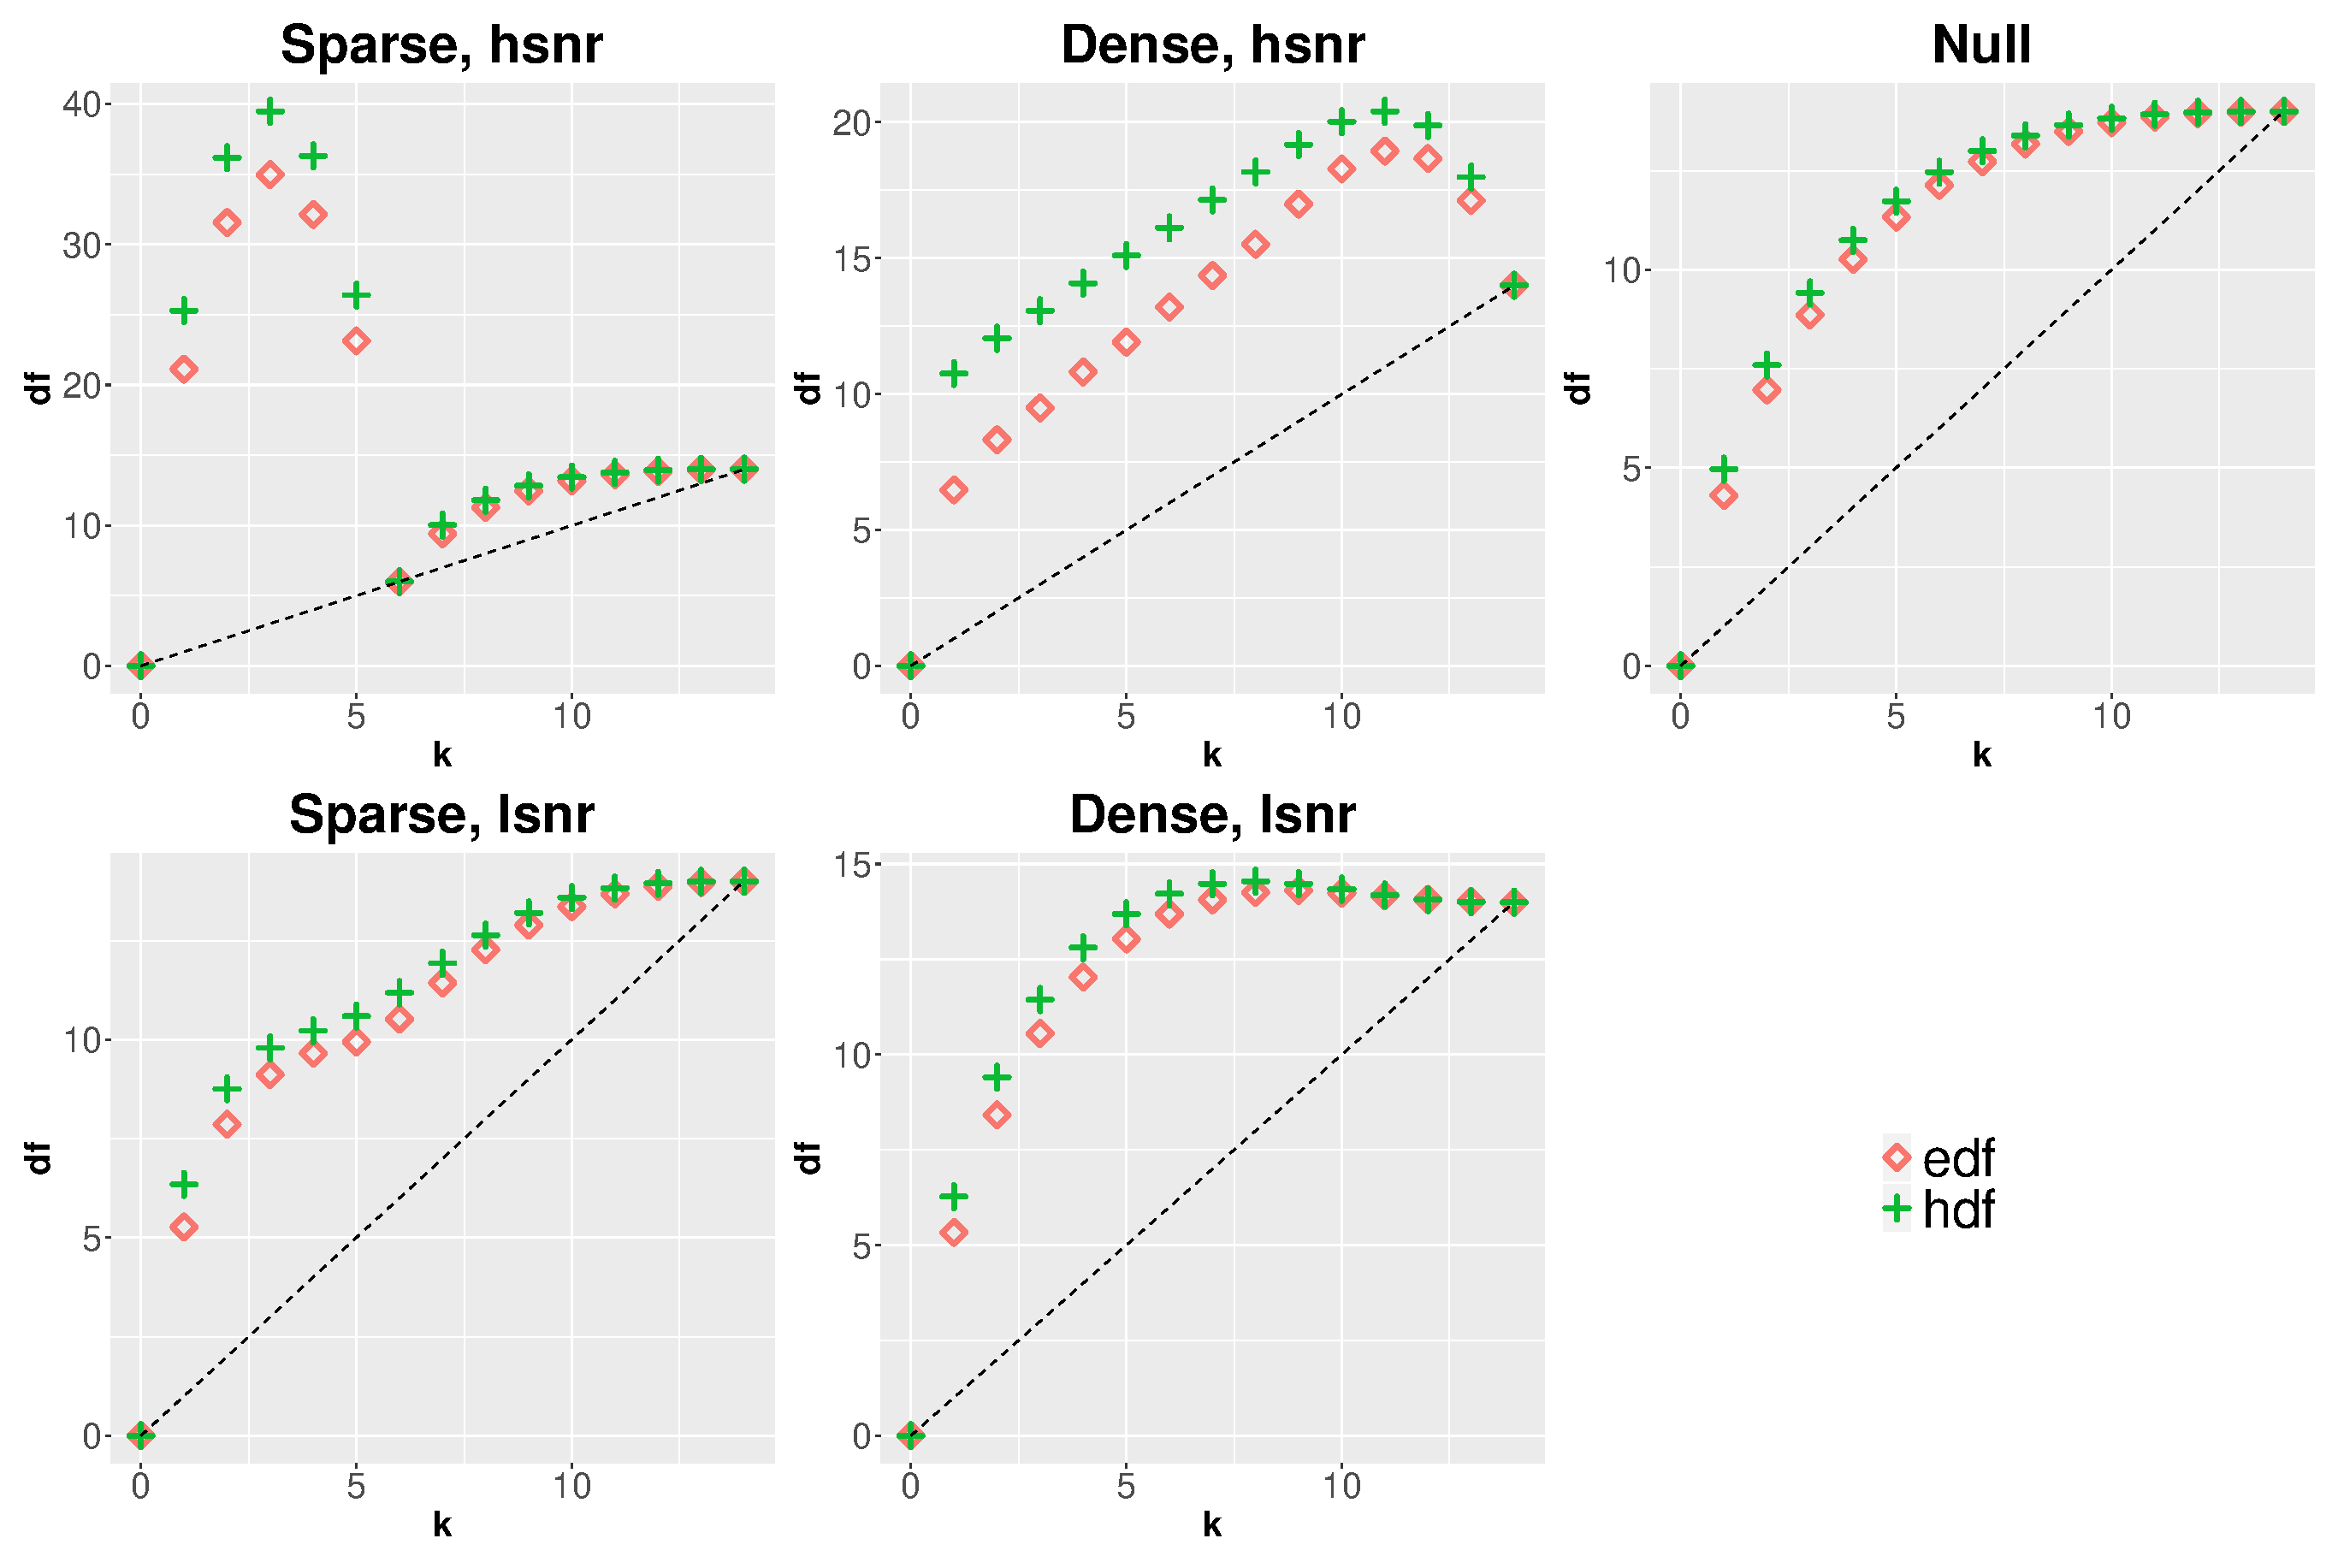
\includegraphics[width=0.9\textwidth]{figures/hdf_edf_bs.eps}
	\caption{hdf$(k)$ and df$_C(k)$ (edf of constrained BS). The black dashed line is the 45-degree line. Here $X$ is orthogonal with $n=200$ and $p=14$. Three types of the true model and two SNR are considered. We assume knowledge of $\mu$ and $\sigma$.}
	\label{fig:dfc_dflambda}
\end{figure}



\subsubsection{\texorpdfstring{C$_p$}{Lg}-hdf as a feasible implementation of \texorpdfstring{C$_p$}{Lg}-edf }
\label{sec:cp_edf_hdf}
We have shown that hdf generally approximates edf well, and it agrees with edf as $k$ approaches $p$. By replacing edf with hdf in \eqref{eq:cp_edf}, we have a feasible selection rule C$_p$-hdf. Figure \ref{fig:cp_edf_hdf} compares the averages of C$_p$-edf and C$_p$-hdf over $1000$ replications. Similarly to the comparison of the degrees of freedom values, we see C$_p$-hdf agrees with C$_p$-edf on averages as $k$ approaches $p$. Even at the places where we see differences between the degrees of freedom values, e.g. a sparse true model with high SNR and $k<p_0=6$, the differences are compensated by the model fit and we see C$_p$-hdf is very close to C$_p$-edf. As we discussed in Section \ref{sec:optimism}, for any general fitting procedure including BS, C$_p$-edf provides an unbiased estimator of the expected prediction error where the error measure $\Theta$ is the squared error (SE), i.e. $E(\text{C}_p\text{-edf}) = E(\text{Err}_{\text{SE}})$. Therefore, by using the sample average to represent the population mean, Figure \ref{fig:cp_edf_hdf} indicates that $E(\text{C}_p\text{-hdf})$ approximates $E(\text{Err}_{\text{SE}})$ well, and moreover C$_p$-hdf gives the same average selected size as C$_p$-edf in all cases, when they are applied as selection rules, supporting the use of hdf in model selection for BS.

% \ref{fig:cp_edf_hdf} 
\begin{figure}[!ht]
	\centering
	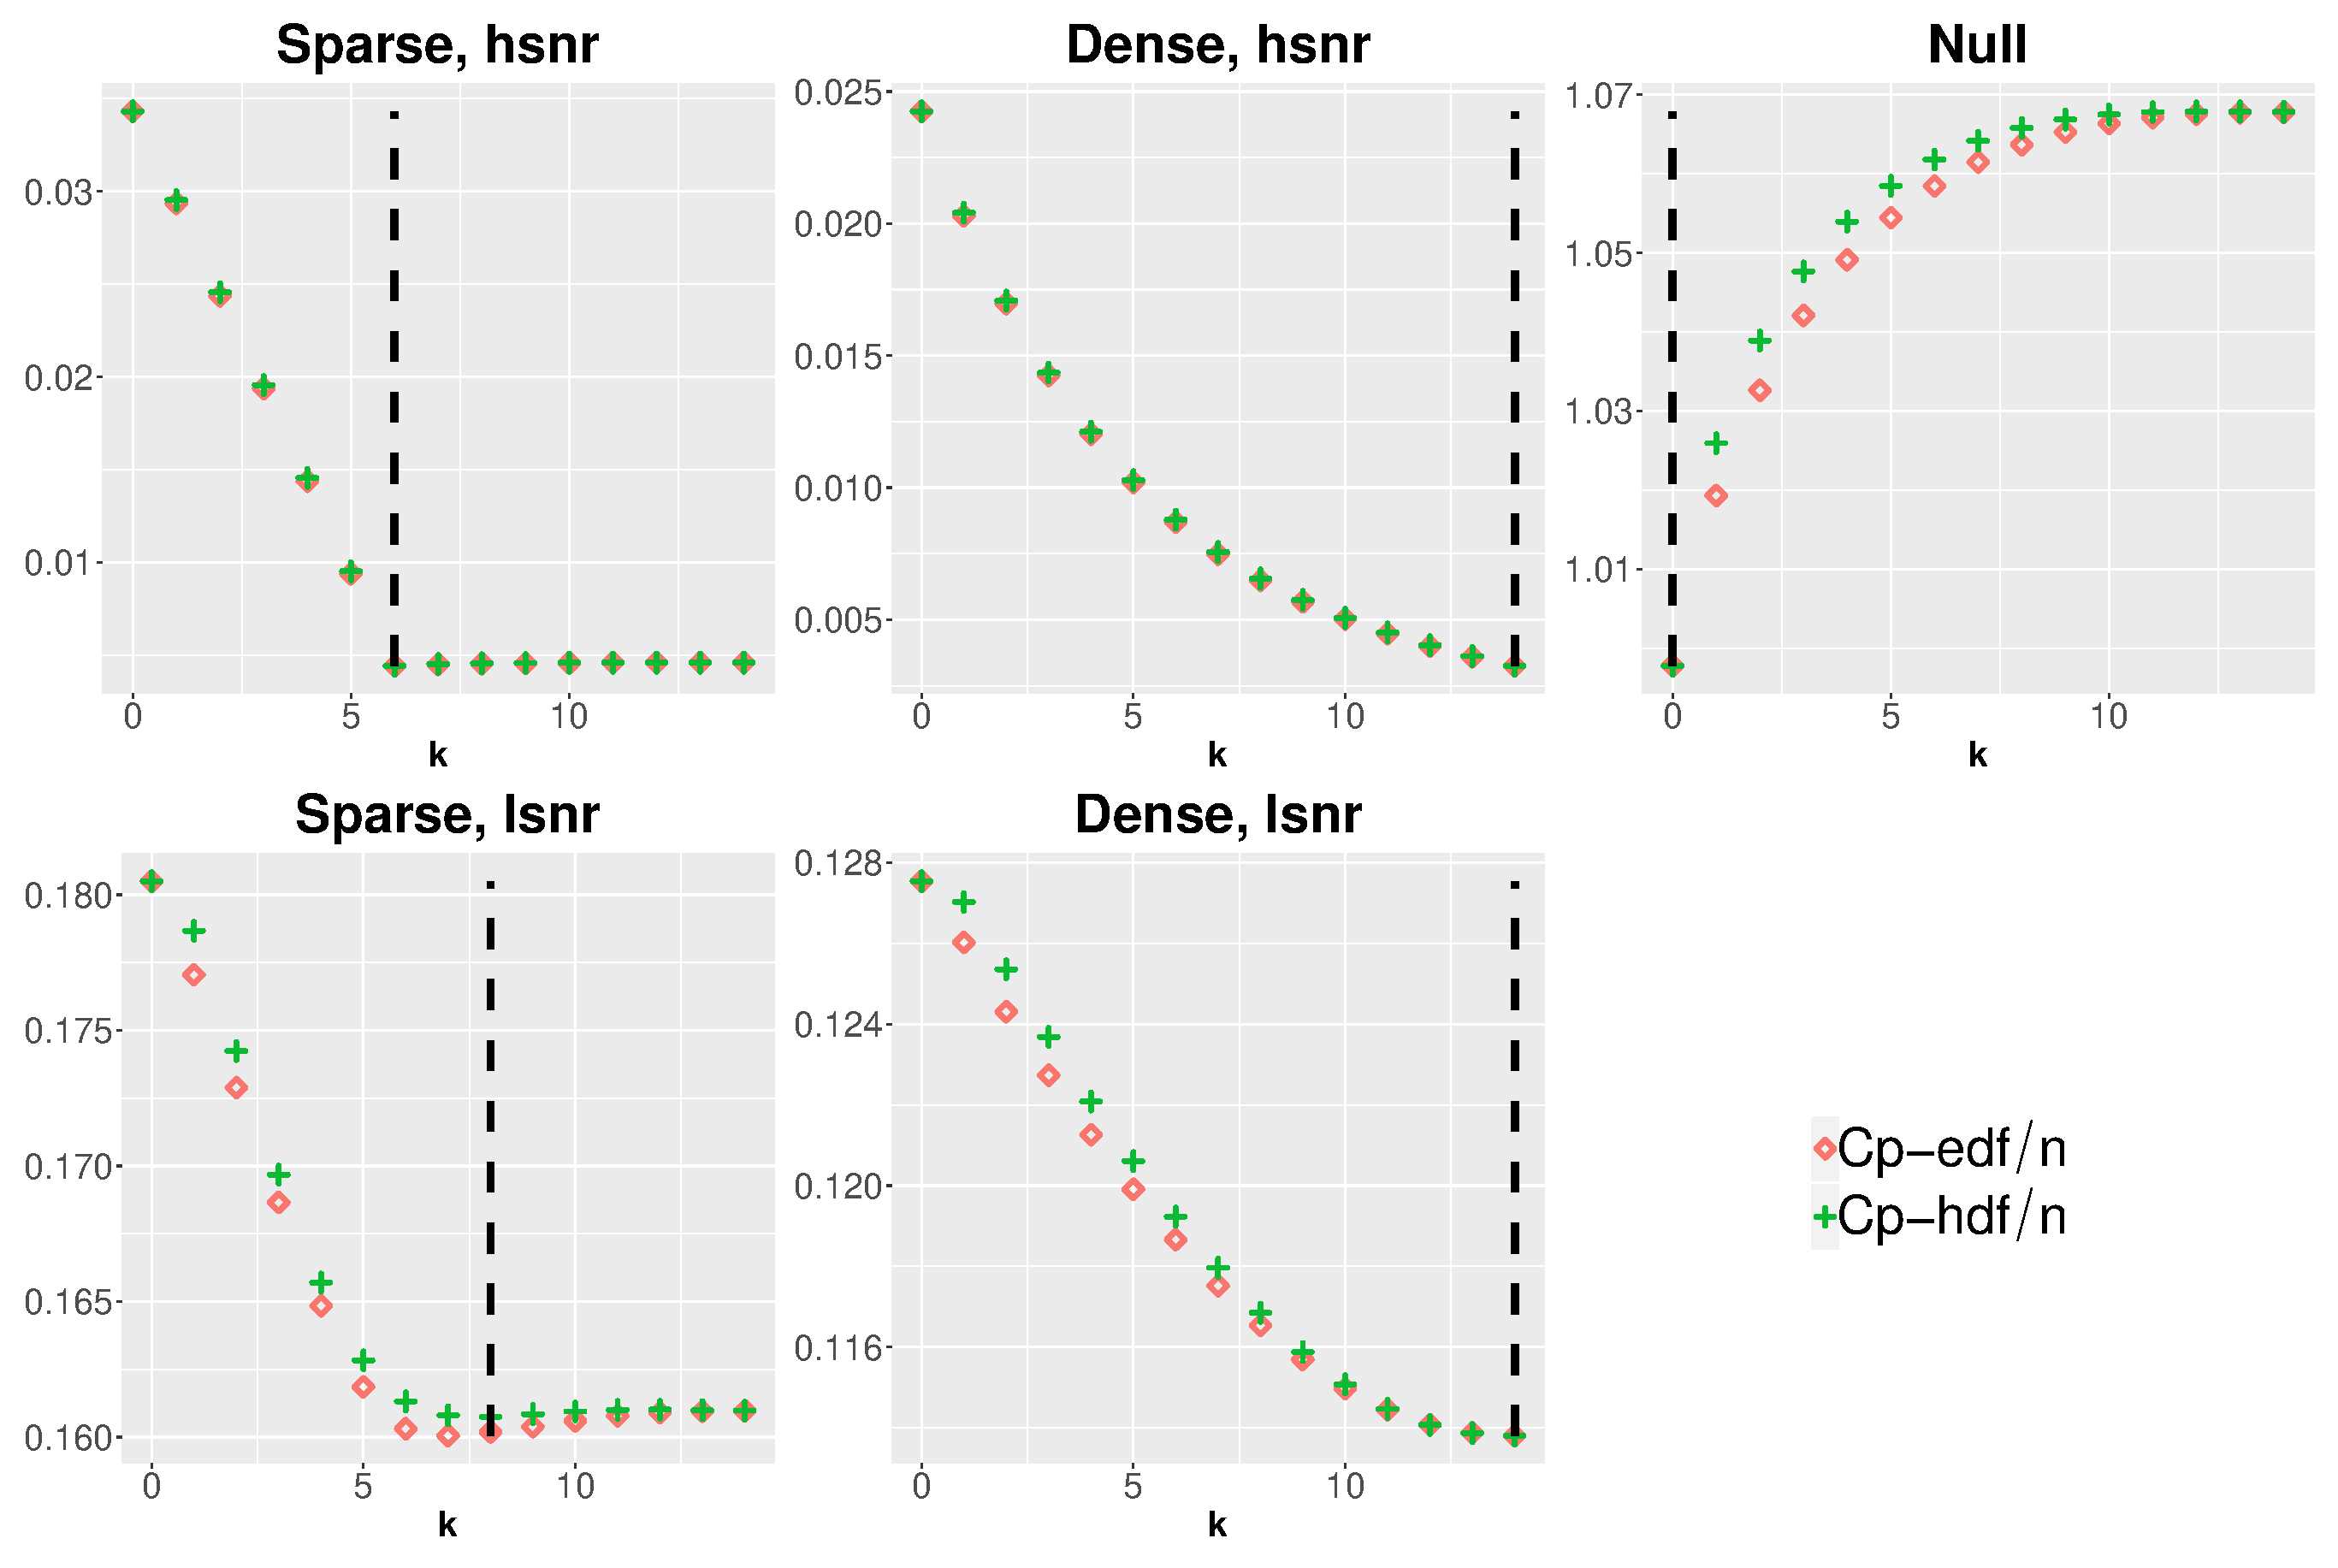
\includegraphics[width=0.9\textwidth]{figures/cp_edf_hdf_bs.eps}
	\caption{Averages of C$_p$-edf and C$_p$-hdf over $1000$ replications. Both criteria lead to the same average of the selected subset size over the $1000$ replications (rounded to the nearest integer), as denoted by the black dashed vertical lines. Other details are the same as in Figure \ref{fig:dfc_dflambda}.}
	\label{fig:cp_edf_hdf} 
\end{figure}


\subsection{A KL-based IC for BS}
When the error measure $\Theta$ is the deviance \eqref{eq:deviance_def}, the prediction error $\text{Err}_\text{KL}$ is the KL discrepancy. AICc-edf \eqref{eq:aicc_edf} is motivated by trying to construct an unbiased estimator of $E(\text{Err}_\text{KL})$. The expected KL-based optimism for BS is given as
\begin{equation}
E(\text{op}_\text{KL}) = E\left(n \frac{n\sigma^2+\lVert \mu-X\hat{\beta}(k) \rVert_2^2}{\lVert y-X\hat{\beta}(k)\rVert_2^2}\right) + n.
\label{eq:eop_expression}
\end{equation}
Note that \eqref{eq:eop_expression} holds for a general $X$. Augmenting $E(\text{op}_\text{KL})$ with the training error $\text{err}_{\text{KL}}$ we have $\widehat{\text{Err}}_{\text{KL}}$ according to \eqref{eq:err_eop}, where (ignoring the constant $n\log(2\pi)$ for convenience)
\begin{equation}
\text{err}_{\text{KL}} = n\log\left(\frac{\text{RSS}}{n}\right) - n,
\label{eq:err_expression}
\end{equation}
since the pre-specified model $f$ in \eqref{eq:deviance_def} follows a Gaussian distribution as assumed in \eqref{eq:truemodel_def}. The derivations of \eqref{eq:eop_expression} and \eqref{eq:err_expression} are presented in the Supplemental Material. 

Figure \ref{fig:eop_approx_withrss} shows the averages of AICc-edf, AICc-hdf (AICc-hdf is calculated by replacing edf with hdf in \eqref{eq:aicc_edf}) and $\widehat{\text{Err}}_{\text{KL}}$ over $1000$ replications. By using the sample average to represent population mean, we first see that $E(\text{AICc-edf})$ generally tracks the expected KL, $E(\text{Err}_{\text{KL}})$ reasonably well. In fact, they agree with each other in the null case and a sparse true model with high SNR. Noticeable discrepancies can be observed in a sparse true model with high SNR and $k<p_0=6$. This is the place where the set of true predictors is not entirely included in the model. The derivations of the classic AIC and AICc (both with ndf plugged in according to our notation) are based on an assumption that the true predictors are included in the model. In the situation where this assumption is violated, AICc will no longer be unbiased, and a similar conjecture can be made here for AICc-edf in the context of BS. Second, similarly to the comparison of $E(\text{C}_p\text{-edf})$ and $E(\text{C}_p\text{-hdf})$ in Section \ref{sec:cp_edf_hdf}, we see that $E(\text{AICc-hdf})$ approximates $E(\text{AICc-edf})$ well and they agree with each other as $k$ approaches $p$. 
Last and most importantly, both AICc-edf and AICc-hdf yield the same average selected size as $\widehat{\text{Err}}_{\text{KL}}$ across all scenarios, supporting the use of AICc-hdf as a selection rule for BS.

% \ref{fig:eop_approx_withrss} 
\begin{figure}[!ht]
	\centering
	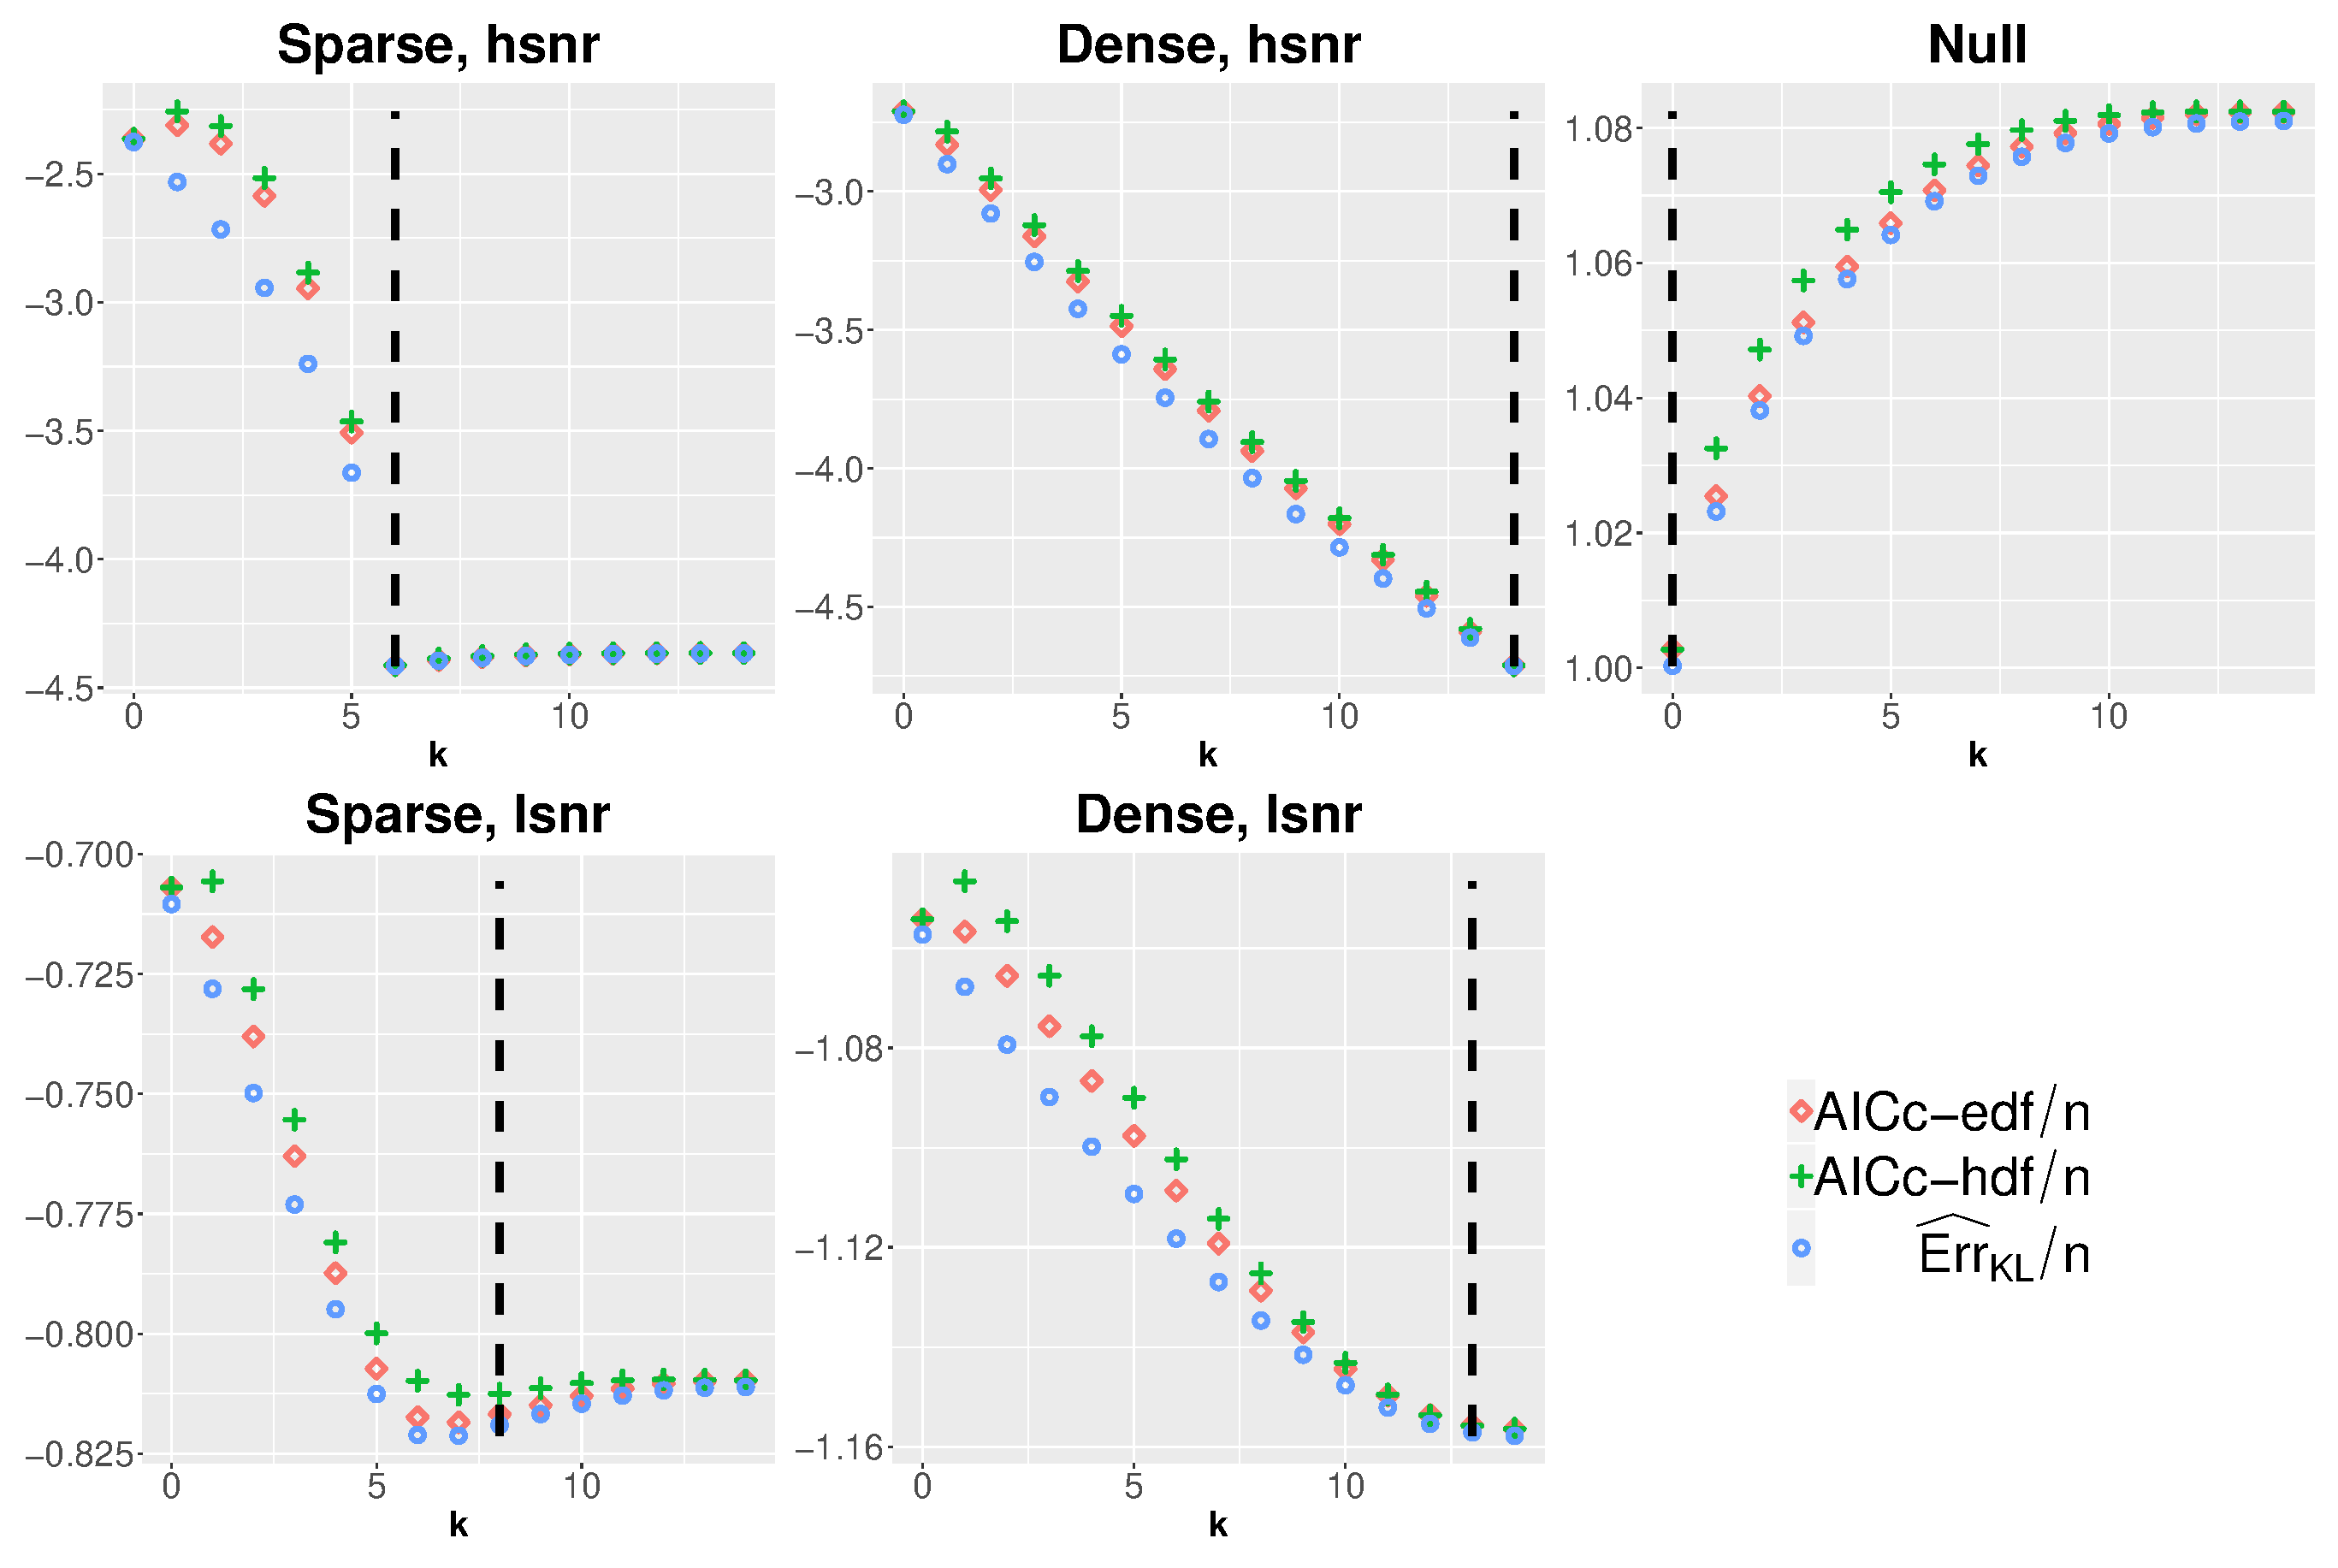
\includegraphics[width=0.9\textwidth]{figures/aicc_edf_hdf_kl_bs.eps}
	\caption{Averages of AICc-edf, AICc-hdf and $\widehat{\text{Err}}_\text{KL}$ over $1000$ replications. All three criteria lead to the same average of the selected subset size over the $1000$ replications (rounded to the nearest integer), as denoted by the black dashed vertical lines. Other details are the same as in Figure \ref{fig:dfc_dflambda}.}
	\label{fig:eop_approx_withrss} 
\end{figure}

\subsection{The performance of AICc-hdf as a selection rule for BS}
We now study the performance of AICc-hdf as a selection rule for BS. The only assumption we make in the simulations is $X$ being orthogonal. Both $\mu$ and $\sigma$ are treated unknown, as would be the case in practice. We start by showing that AICc-hdf can perform well for BS compared to other selection rules. We then compare the performance of BS-AICc-hdf to that of regularization methods. 

\subsubsection{Simulation set-up}
\label{sec:simulation_setup_orthx}
We consider a trigonometric configuration of $X$ that is studied by \citet{Hurvich1991}, where $X=(x^1,x^2)$ is an $n$ by $p$ matrix with components defined by 
$$ x_{tj}^1 = \sin\left(\frac{2\pi j}{n}t\right),$$
and 
$$ x_{tj}^2 = \cos\left(\frac{2\pi j}{n}t\right),$$
for $j=1,\cdots,p/2$ and $t=0,\cdots,n-1$. The columns of $X$ are then standardized to have $l_2$ norm 1, to make them orthonormal. By fixing $X$, the responses are generated by \eqref{eq:truemodel_def}, where $\mu=X\beta$. The error $\epsilon$ is also shifted to have mean $0$, hence the intercept will be zero. 

We consider the following configurations of the experiment:
\begin{itemize}
	\item Sample size: $n \in \{200, 2000\}$.
	\item Number of predictors: $p \in \{14,30,60,180\}$.
	\item Signal-to-noise ratio: $\text{SNR} \in \{0.2,1.5,7\}$ (low, medium and high). The average oracle $R^2$ (linear regression on the set of true predictors) corresponding to these three SNR values are roughly $20\%$, $50\%$ and $90\%$, respectively.
	\item Coefficient vector $\beta$ (Orth in the following denotes for orthogonal $X$):
	\begin{itemize}
		\item Orth-Sparse-Ex1: $\beta=[1_6,0_{p-6}]^T$
		\item Orth-Sparse-Ex2: $\beta=[1,-1,5,-5,10,-10,0_{p-6}]^T$
		\item Orth-Dense \citep{Taddy2017}: $\beta_j = (-1)^j \exp(-\frac{j}{\kappa})$, $j=1,\cdots,p$. $\kappa=10$ 
		%\item Dense-Ex2: same definition of $\beta$ as in Dense-Ex1, but with $\kappa=50$
	\end{itemize}
\end{itemize}

\iffalse
Note that all of the coefficients in the dense designs are non-zero, but many of them have little effects. Dense-Ex1 has a fast decay where only $23$ coefficients have absolute values larger than $0.1$, while the slow decay Dense-Ex2 has $115$ coefficients larger than $0.1$. The dense designs are introduced by \citet{Taddy2017}.
\fi

In total, there are $72$ different scenarios in the experiment. The full set of simulation results is presented in the Supplemental Material. In each scenario, $1000$ replications of the response $y$ are generated. A fitting procedure $\hat{\mu}$, is evaluated via the average RMSE, where 
\begin{equation}
\text{RMSE}(\hat{\mu}) = \sqrt{ \frac{1}{n} \lVert \hat{\mu}-X\beta \rVert_2^2}.
\label{eq:l2_loss}
\end{equation}
To make the scales easier to compare, we construct two relative metrics: $\%$ worse than the best possible BS, and relative efficiency, which are defined as follows:
\begin{itemize}
	\item \textbf{$\%$ worse than best possible BS}
	\begin{equation} 
	=\displaystyle 100 \times \left( \frac{\text{averge RMSE of a fitting procedure } \hat{\mu}}{\text{average RMSE of the best possible BS}} - 1 \right) \%,
	\end{equation}
	where the best possible BS here means that on a single fit, choosing the subset size with the minimum RMSE among all $p+1$ candidates, as if an oracle tells us the true model.
	
	\item \textbf{Relative efficiency:} For a collection of fitting procedures, the relative efficiency for a particular procedure $j$, is defined as
	\begin{equation}
	\displaystyle \frac{\min_l \text{ average RMSE of fitting procedure }l}{\text{average RMSE of fitting procedure }j}.
	\end{equation}
	The relative efficiency is a measure between $0$ and $1$. Higher value indicates better performance. Besides the fitting procedures specified, we include the null and full OLS in the calculation of relative efficiency. 
\end{itemize}
We also present the sparsistency (number of true positives) and number of extra predictors (number of false positives). 


\subsubsection{AICc-hdf and other selection rules for BS}
\label{sec:bs_ic_simulationresults}
By analogy to C$_p$ and AICc, we can also define BIC-edf as
\begin{equation}
\text{BIC-edf} = n \log\left(\frac{\text{RSS}}{n}\right) + \log(n) \cdot \text{edf},
\label{eq:bic_edf}
\end{equation}
and its feasible version BIC-hdf, where the original BIC (or BIC-ndf in our notation) was introduced in \citet{schwarz1978estimating}. We also consider a numerical estimation of edf that is based on the parametric bootstrap, and we denote it as bdf. The detailed implementation of bdf and the benefit of parametric bootstrap is discussed in \citet{Efron2004}. In our experiment, we use $100$ bootstrapped samples. In addition to the information criteria, we further include 10-fold cross-validation (CV) for comparison. Note that the CV results are only available for $p \le 30$ since it is fitted using the `leaps' algorithm.

A selected set of results is shown in Tables \ref{tab:ic_df_orthx_sparseex1} and \ref{tab:ic_df_orthx_dense}. A brief summary is as follows:
\begin{itemize}
	\item Using information criteria in the naive way (with ndf) can be dangerous, especially when $p$ is large and SNR is high. For example, using ndf in AICc significantly overfits and can be almost $400$ times worse in terms of RMSE than using hdf for $n=200$, high SNR and $p=180$ in Orth-Sparse-Ex1. Increasing the sample size $n$ does not improve IC-ndf, and the overfiting persists.
	\item AICc-hdf generally does not lose much efficiency and performs similarly in terms of RMSE, in comparison to the infeasible AICc-edf. Increasing the sample size $n$ or SNR improves the performance of both AICc-edf and AICc-hdf. 
	\item AICc-hdf performs very similarly to AICc-bdf. Since bdf is calculated based on $100$ bootstrapped samples, it is roughly $100$ times more intensive than hdf in computations. 
	\item AICc-hdf is generally better than 10-fold CV, e.g. when $n$ is large or SNR is high. Note that 10-fold CV is roughly $10$ times heavier in terms of computation than AICc-hdf. It is also worth noticing that these findings are broadly consistent with the results reported by \citet{Taddy2017} for the Gamma LASSO method. 
	\item C$_p$-edf performs similarly to AICc-edf. In contrast, when we consider the feasible implementations (ndf/hdf/bdf), i.e. when $\sigma$ is estimated by full OLS, C$_p$ can suffer when $p$ is close to $n$, such as when $n=200$ and $p=180$. Under a sparse true model BIC-hdf performs slightly better than AICc-hdf except when SNR is low and $n=200$, where BIC is considerably worse. Under a dense true model BIC-hdf is always outperformed by AICc-hdf. 
\end{itemize}
For the reasons presented above, we conclude that AICc-hdf is the best feasible selection rule for BS, among all that have been considered.

% {tab:ic_df_orthx_sparseex1}
% latex table generated in R 3.6.1 by xtable 1.8-4 package
% Sun Nov 10 00:43:00 2019
\begin{table}[ht]
\centering
\caption{The performance of AICc-hdf. The true model setup is Orth-Sparse-Ex1. 
                    The columns involving `edf' refer to infeasible selection rules since edf is estimated as if the true model is known, 
                    while other columns correspond to feasible rules.} 
\label{tab:ic_df_orthx_sparseex1}
\scalebox{0.65}{
\begin{tabular}{|c|c|c|cc|cc|cc|c|}
  \toprule 
 \multicolumn{1}{|r}{} & \multicolumn{1}{c}{} &       & \multicolumn{2}{c|}{C$_p$} & \multicolumn{2}{c|}{AICc} & \multicolumn{2}{c|}{BIC} & \multirow{2}[4]{*}{CV} \\
 \cmidrule{4-9}\multicolumn{1}{|r}{} & \multicolumn{1}{c}{} &       & edf   & ndf/hdf/bdf & edf   & ndf/hdf/bdf & edf   & ndf/hdf/bdf &     \\
 \midrule 
 \multicolumn{1}{|r}{} & \multicolumn{1}{c}{} &       & \multicolumn{7}{c|}{\% worse than the best possible BS} \\
 \midrule 
 \multirow{4}[4]{*}{n=200} & \multirow{2}[2]{*}{hsnr} & p=30 & 4 & 84/5/7 & 2 & 83/2/5 & 0 & 28/0/0 & 24 \\ 
   &  & p=180 & 1 & 338/30/32 & 0 & 392/1/2 & 0 & 206/0/0 & - \\ 
  \cmidrule{2-10} & \multirow{2}[2]{*}{lsnr} & p=30 & 20 & 25/36/33 & 21 & 24/37/35 & 68 & 23/68/67 & 28 \\ 
   &  & p=180 & 15 & 108/35/34 & 18 & 132/22/22 & 25 & 50/25/25 & - \\ 
  \midrule \multirow{4}[4]{*}{n=2000} & \multirow{2}[2]{*}{hsnr} & p=30 & 3 & 85/3/6 & 3 & 85/3/6 & 0 & 9/0/0 & 23 \\ 
   &  & p=180 & 0 & 334/1/3 & 1 & 337/1/3 & 0 & 60/0/0 & - \\ 
  \cmidrule{2-10} & \multirow{2}[2]{*}{lsnr} & p=30 & 3 & 85/6/7 & 3 & 85/5/6 & 0 & 9/0/0 & 23 \\ 
   &  & p=180 & 0 & 334/5/4 & 1 & 337/4/4 & 0 & 60/1/1 & - \\ 
   \midrule 
 \multicolumn{1}{|r}{} & \multicolumn{1}{r}{} &       & \multicolumn{7}{c|}{Relative efficiency} \\
 \midrule 
\multirow{4}[4]{*}{n=200} & \multirow{2}[2]{*}{hsnr} & p=30 & 0.96 & 0.54/0.95/0.93 & 0.98 & 0.55/0.98/0.96 & 1 & 0.78/1/1 & 0.81 \\ 
   &  & p=180 & 0.99 & 0.23/0.77/0.76 & 1 & 0.2/0.99/0.98 & 1 & 0.33/1/1 & - \\ 
  \cmidrule{2-10} & \multirow{2}[2]{*}{lsnr} & p=30 & 1 & 0.97/0.89/0.9 & 1 & 0.97/0.88/0.89 & 0.72 & 0.98/0.72/0.72 & 0.94 \\ 
   &  & p=180 & 1 & 0.55/0.86/0.86 & 0.97 & 0.5/0.95/0.95 & 0.93 & 0.77/0.93/0.93 & - \\ 
  \midrule \multirow{4}[4]{*}{n=2000} & \multirow{2}[2]{*}{hsnr} & p=30 & 0.97 & 0.54/0.97/0.94 & 0.97 & 0.54/0.97/0.94 & 1 & 0.92/1/1 & 0.81 \\ 
   &  & p=180 & 1 & 0.23/0.99/0.97 & 0.99 & 0.23/0.99/0.97 & 1 & 0.62/1/1 & - \\ 
  \cmidrule{2-10} & \multirow{2}[2]{*}{lsnr} & p=30 & 0.97 & 0.54/0.95/0.94 & 0.97 & 0.54/0.95/0.94 & 1 & 0.92/1/1 & 0.81 \\ 
   &  & p=180 & 1 & 0.23/0.96/0.96 & 0.99 & 0.23/0.96/0.96 & 1 & 0.62/0.99/0.99 & - \\ 
   \midrule 
 \multicolumn{1}{|r}{} & \multicolumn{1}{r}{} &       & \multicolumn{7}{c|}{Sparsistency (number of extra variables)} \\
 \midrule 
\multirow{4}[4]{*}{n=200} & \multirow{2}[2]{*}{hsnr} & p=30 & 6(0.1) & 6(3.9)/6(0.2)/6(0.2) & 6(0) & 6(3.8)/6(0.1)/6(0.1) & 6(0) & 6(0.6)/6(0)/6(0) & 6(0.7) \\ 
   &  & p=180 & 6(0) & 6(32.2)/6(6.4)/6(6.3) & 6(0) & 6(48.9)/6(0)/6(0) & 6(0) & 6(9.5)/6(0)/6(0) & - \\ 
  \cmidrule{2-10} & \multirow{2}[2]{*}{lsnr} & p=30 & 4.5(1.9) & 5.3(3.9)/4.2(4.9)/4.2(4) & 4.2(1.2) & 5.2(3.8)/3.3(2.2)/3.4(1.8) & 0.1(0) & 3.7(0.6)/0.1(0)/0.2(0) & 4(1.9) \\ 
   &  & p=180 & 1.9(0.5) & 5.3(32.2)/1.8(10.9)/1.9(9.8) & 1.1(0.1) & 5.6(49)/0.5(0)/0.6(0) & 0(0) & 4.2(8.4)/0(0)/0(0) & - \\ 
  \midrule \multirow{4}[4]{*}{n=2000} & \multirow{2}[2]{*}{hsnr} & p=30 & 6(0.1) & 6(3.8)/6(0.1)/6(0.2) & 6(0.1) & 6(3.8)/6(0.1)/6(0.2) & 6(0) & 6(0.1)/6(0)/6(0) & 6(0.6) \\ 
   &  & p=180 & 6(0) & 6(27.5)/6(0)/6(0) & 6(0) & 6(28.2)/6(0)/6(0) & 6(0) & 6(1.1)/6(0)/6(0) & - \\ 
  \cmidrule{2-10} & \multirow{2}[2]{*}{lsnr} & p=30 & 6(0.1) & 6(3.8)/6(0.2)/6(0.2) & 6(0.1) & 6(3.8)/6(0.2)/6(0.2) & 6(0) & 6(0.1)/6(0)/6(0) & 6(0.6) \\ 
   &  & p=180 & 6(0) & 6(27.5)/6(0.1)/6(0) & 6(0) & 6(28.2)/6(0.1)/6(0) & 6(0) & 6(1.1)/6(0)/6(0) & - \\ 
   \bottomrule 
\end{tabular}
}
\end{table}


% {tab:ic_df_orthx_dense}
% latex table generated in R 3.6.1 by xtable 1.8-4 package
% Sun Nov 10 00:46:50 2019
\begin{table}[ht]
\centering
\caption{Information criteria for BS under orthogonal $X$. The true model setup is Orth-Dense (see Supplemental Material Section \ref{sec:simulation_setup_orthx} for details).} 
\label{tab:ic_df_orthx_dense}
\scalebox{0.7}{
\begin{tabular}{|c|c|c|cc|cc|cc|c|}
  \toprule 
 \multicolumn{1}{|r}{} & \multicolumn{1}{c}{} &       & \multicolumn{2}{c|}{C$_p$} & \multicolumn{2}{c|}{AICc} & \multicolumn{2}{c|}{BIC} & \multirow{2}[4]{*}{CV} \\
 \cmidrule{4-9}\multicolumn{1}{|r}{} & \multicolumn{1}{c}{} &       & edf   & ndf/hdf/bdf & edf   & ndf/hdf/bdf & edf   & ndf/hdf/bdf &     \\
 \midrule 
 \multicolumn{1}{|r}{} & \multicolumn{1}{c}{} &       & \multicolumn{7}{c|}{\% worse than the best possible BS} \\
 \midrule 
 \multirow{4}[4]{*}{n=200} & \multirow{2}[2]{*}{hsnr} & p=30 & 1 & 11/1/2 & 1 & 13/1/2 & 1 & 28/3/5 & 7 \\ 
   &  & p=180 & 7 & 45/21/20 & 9 & 52/18/19 & 18 & 26/39/42 & - \\ 
  \cmidrule{2-10} & \multirow{2}[2]{*}{lsnr} & p=30 & 15 & 10/16/16 & 20 & 10/21/20 & 27 & 16/27/27 & 16 \\ 
   &  & p=180 & 8 & 86/22/22 & 7 & 102/7/7 & 7 & 39/7/7 & - \\ 
  \midrule \multirow{4}[4]{*}{n=2000} & \multirow{2}[2]{*}{hsnr} & p=30 & 0 & 1/0/0 & 0 & 1/0/0 & 0 & 18/0/1 & 1 \\ 
   &  & p=180 & 6 & 34/8/8 & 6 & 34/8/8 & 19 & 7/36/37 & - \\ 
  \cmidrule{2-10} & \multirow{2}[2]{*}{lsnr} & p=30 & 2 & 11/3/3 & 2 & 11/3/3 & 44 & 41/36/45 & 10 \\ 
   &  & p=180 & 8 & 48/10/10 & 8 & 48/10/10 & 24 & 8/45/47 & - \\ 
   \midrule 
 \multicolumn{1}{|r}{} & \multicolumn{1}{r}{} &       & \multicolumn{7}{c|}{Relative efficiency} \\
 \midrule 
\multirow{4}[4]{*}{n=200} & \multirow{2}[2]{*}{hsnr} & p=30 & 1 & 0.91/1/1 & 1 & 0.9/1/0.99 & 1 & 0.79/0.98/0.96 & 0.95 \\ 
   &  & p=180 & 1 & 0.74/0.89/0.89 & 0.99 & 0.71/0.91/0.9 & 0.91 & 0.85/0.77/0.76 & - \\ 
  \cmidrule{2-10} & \multirow{2}[2]{*}{lsnr} & p=30 & 0.95 & 1/0.95/0.95 & 0.91 & 1/0.91/0.91 & 0.86 & 0.94/0.86/0.86 & 0.94 \\ 
   &  & p=180 & 1 & 0.58/0.88/0.88 & 1 & 0.53/1/1 & 1 & 0.77/1/1 & - \\ 
  \midrule \multirow{4}[4]{*}{n=2000} & \multirow{2}[2]{*}{hsnr} & p=30 & 1 & 0.99/1/1 & 1 & 0.99/1/1 & 1 & 0.85/1/0.99 & 0.99 \\ 
   &  & p=180 & 1 & 0.79/0.98/0.98 & 1 & 0.79/0.98/0.98 & 0.89 & 1/0.78/0.78 & - \\ 
  \cmidrule{2-10} & \multirow{2}[2]{*}{lsnr} & p=30 & 1 & 0.92/0.99/0.99 & 1 & 0.92/0.99/0.99 & 0.71 & 0.73/0.75/0.7 & 0.93 \\ 
   &  & p=180 & 1 & 0.73/0.98/0.98 & 1 & 0.73/0.98/0.98 & 0.87 & 1/0.74/0.73 & - \\ 
   \midrule 
 \multicolumn{1}{|r}{} & \multicolumn{1}{r}{} &       & \multicolumn{7}{c|}{Sparsistency (number of extra variables)} \\
 \midrule 
\multirow{4}[4]{*}{n=200} & \multirow{2}[2]{*}{hsnr} & p=30 & 30 & 24.7/29.5/29 & 30 & 24.2/29.4/28.8 & 30 & 20.9/28.8/27.5 & 26.6 \\ 
   &  & p=180 & 20.5 & 53.3/37.4/35.5 & 18.3 & 62.3/16.3/16.3 & 16.1 & 35/13.7/13.5 & - \\ 
  \cmidrule{2-10} & \multirow{2}[2]{*}{lsnr} & p=30 & 12.8 & 10.5/14.6/13 & 7.6 & 10.3/8.5/7.6 & 0 & 4/0/0 & 7.5 \\ 
   &  & p=180 & 0.8 & 39/14.5/13.7 & 0.3 & 55.2/0.2/0.3 & 0 & 11.8/0/0 & - \\ 
  \midrule \multirow{4}[4]{*}{n=2000} & \multirow{2}[2]{*}{hsnr} & p=30 & 30 & 29.8/30/29.9 & 30 & 29.8/30/29.9 & 30 & 28.6/30/29.9 & 29.8 \\ 
   &  & p=180 & 32.1 & 58.9/32.4/32.3 & 31.8 & 58.9/31.6/31.6 & 27 & 31.3/25/24.9 & - \\ 
  \cmidrule{2-10} & \multirow{2}[2]{*}{lsnr} & p=30 & 28.8 & 19.9/28.2/26.9 & 28.8 & 19.9/28.1/26.8 & 13.5 & 12.5/16.7/14.1 & 22.3 \\ 
   &  & p=180 & 13.9 & 43.8/14/14 & 13.6 & 44.1/13.3/13.3 & 9.1 & 13.4/7/6.8 & - \\ 
   \bottomrule 
\end{tabular}
}
\end{table}



\subsubsection{How does BS perform compared to regularization methods?}
\label{sec:bs_regu}
We have seen that AICc-hdf can be an effective selection rule for BS. In this section, we compare BS with some popular regularization methods, including LASSO \citep{Tibshirani1996}, SparseNet \citep{Mazumder2011}, Gamma LASSO \citep{Taddy2017} and relaxed LASSO \citep{Meinshausen2007}. We use {\tt{R}} packages \pkg{glmnet} \citep{Friedman2010}, \pkg{sparsenet} \citep{Mazumder2011}, \pkg{gamlr} \citep{Taddy2017} and \pkg{relaxo} \citep{Meinshausen2012}, to fit them, respectively, which are all available on \textit{CRAN}.

\iffalse
The penalized regression methods shrink the coefficient estimates towards zero and can provide sparse solutions. They apply different penalty functions. LASSO, which at parameter $\lambda \ge 0$ solves
\begin{equation}
\argmin_\beta \frac{1}{2} \lVert y-X\beta \rVert_2^2 + \lambda \lVert \beta \rVert_1,
\label{eq:lasso}
\end{equation}
applies a $l_1$ penalty. SparseNet at parameters $\lambda \ge 0$ and $\gamma \ge 0$, is a solver for the MCP penalty \citep{Zhang2010}:
\begin{equation}
\argmin_\beta \frac{1}{2} \lVert y-X\beta \rVert_2^2 + \sum_{j=1}^p \lambda \int_{0}^{|\beta_j|} (1-\frac{x}{\gamma \lambda})_+ dx.
\label{eq:mcp}
\end{equation} 
Gamma LASSO applies a log penalty, and at parameters $\lambda \ge 0$ and $\gamma \ge 0$ it solves
\begin{equation}
\argmin_\beta \frac{1}{2} \lVert y-X\beta \rVert_2^2 + \sum_{j=1}^{p} \frac{\lambda}{\gamma} \log(1+\gamma |\beta_j|).
\label{eq:gamlr}
\end{equation}
Finally, the simplified relaxed LASSO was studied in \citet{Hastie2017}. We will drop 'simplified' and refer it as relaxed LASSO. Denote $\hat{\beta}^\text{LASSO}(\lambda)$ as the LASSO solution at parameter $\lambda$, $S_\lambda$ as the support of predictors with non-zero coefficients, and $\hat{\beta}^\text{LS}(\lambda)$ as the LS estimates of regressing $y$ upon $X_{S_\lambda}$ with zeroes filling in places of $\{1,\cdots,p\} \setminus S_\lambda$. The relaxed LASSO estimate at parameters $\lambda \ge 0$ and $\gamma \in [0,1]$ is a trade-off between the LASSO and LS estimates:
\begin{equation}
\gamma \hat{\beta}^\text{LASSO}(\lambda) + (1-\gamma) \hat{\beta}^\text{LS}(\lambda).
\label{eq:rlasso}
\end{equation}
Due to the attractive convex property, LASSO \eqref{eq:lasso} has been a popular method throughout the literature. It's also known to tend to over-shrink the retained predictors, in order to maintain the sparsity. On the other hand, the non-convex penalized methods, e.g. \eqref{eq:mcp} and \eqref{eq:gamlr}, are designed to yield sparse solutions while preserving little bias for large non-zero estimates. Parameter $\lambda$ in these methods decide the level of shrinkage, while $\gamma$ in the non-convex penalized methods controls the non-convexity. For example, \eqref{eq:mcp} corresponds to LASSO \eqref{eq:lasso} when $\gamma \rightarrow \infty$ and it becomes LBS \eqref{eq:lbestsubset-setup} when $\gamma \rightarrow 1$. Parameter $\gamma$ in the relaxed LASSO has the purpose of reducing the level of shrinkage being applied on the retained predictors. The relaxed LASSO corresponds to the LS solution when $\gamma = 1$ and equals to the LASSO solution when $\gamma=0$. 
\fi

As to the selection rule, we use AICc-hdf for BS, AICc for LASSO, and 10-fold CV for the rest. In addition to these selectors, we have also considered 10-fold CV for LASSO. We find (in the Supplement) that 10-fold CV performs similarly to AICc for LASSO. In fact, the use of AICc for LASSO has been explored in \citet{Flynn2013}, where the authors proved that AICc is asymptotically efficient while performing similarly to CV. We further notice (results given in the Supplement) that SparseNet generally performs better than the relaxed LASSO and Gamma LASSO, and hence only the results for SparseNet will be presented here. 

A selected set of results is presented in Table \ref{tab:bs_regularization}. A brief summary is as follows:
\begin{itemize}
	\item For a relatively small sample size $n=200$ and a sparse true model, BS performs the best when SNR is high,  LASSO is best in low SNR, and SparseNet has performance in between of the other two methods. LASSO has the property of `over-select and shrink,' in order to retain less bias on the large non-zero estimates. In a high SNR, this property can result in disastrous performance, especially when $p$ is close to $n$. For example, in Orth-Sparse-Ex1, high SNR and $p=180$, the relative efficiency of LASSO is only $0.44$ and it significantly overfits. However, this property can be beneficial when SNR is low, as a method like BS has higher chance to miss the true predictors (less sparsistency).
	
	\item With $n=200$ and a dense true model, the methods perform similarly when SNR is high, while LASSO is better in low SNR.
	
	\item With a large sample size $n=2000$ relative to the values of $p$, BS becomes the best in almost all scenarios. The only exception is when the true model is dense and SNR is low, where BS is very close to the best. In fact, all three methods benefit from increasing $n$, since we can see larger sparsistency and fewer extra variables. Given that, it seems that BS profits the most according to the boost of its relative performance in low SNR. 
\end{itemize}

Given the spirit of the summary above, it's important to point out the relevant work of \citet{Hastie2017}, where the authors provide a comprehensive set of simulation comparisons on BS, LASSO and relaxed LASSO. The authors concluded that BS performs the best in high SNR, LASSO is the best in low SNR while relaxed LASSO is in between. This coincides with the results here when sample size is relatively small ($n=200$), given the similarity in the performance of relaxed LASSO and SparseNet. However, we find BS to be the best for large sample size $n$ even when the SNR is low (note that \citet{Hastie2017} did not examine any sample sizes greater than $n=500$). Moreover, it should be noted that \citet{Hastie2017} focus on the best possible performance of each method by applying a separate validation set drawn from the true model, rather than on feasible selection, as is considered in this study. 

% {tab:bs_regularization}
% latex table generated in R 3.6.1 by xtable 1.8-4 package
% Sun Nov 10 00:54:17 2019
\begin{table}[ht]
\centering
\caption{The performance of BS compared to regularization methods. The selection rules are AICc-hdf for BS, 
		AICc for lasso and 10-fold CV for SparseNet, respectively.} 
\label{tab:bs_regularization}
\scalebox{0.7}{
\begin{tabular}{|c|c|c|ccc|ccc|ccc|}
  \toprule 
 \multicolumn{1}{|r}{} & \multicolumn{1}{r}{} &       & \multicolumn{3}{c|}{Orth-Sparse-Ex1}   & \multicolumn{3}{c|}{Orth-Sparse-Ex2}             & \multicolumn{3}{c|}{Orth-Dense} \\
 \cmidrule{4-12}\multicolumn{1}{|c}{} & \multicolumn{1}{c}{} &       & BS    & lasso & SparseNet & BS    & lasso & SparseNet & BS    & lasso & SparseNet  \\
 \midrule 
 \multicolumn{1}{|c}{} & \multicolumn{1}{c}{} &       & \multicolumn{9}{c|}{\% worse than the best possible BS}  \\
 \midrule 
 \multirow{4}[4]{*}{n=200} & \multirow{2}[2]{*}{hsnr} & p=30 & 2 & 70 & 14 & 25 & 32 & 19 & 1 & 1 & 4 \\ 
   &  & p=180 & 1 & 128 & 20 & 11 & 51 & 14 & 18 & 23 & 7 \\ 
  \cmidrule{2-12} & \multirow{2}[2]{*}{lsnr} & p=30 & 37 & 7 & 15 & 34 & 21 & 25 & 21 & -6 & -2 \\ 
   &  & p=180 & 22 & 1 & 8 & 39 & 24 & 25 & 7 & -2 & 2 \\ 
  \midrule \multirow{4}[4]{*}{n=2000} & \multirow{2}[2]{*}{hsnr} & p=30 & 3 & 70 & 14 & 5 & 71 & 15 & 0 & 1 & 1 \\ 
   &  & p=180 & 1 & 130 & 14 & 4 & 129 & 14 & 8 & 17 & 3 \\ 
  \cmidrule{2-12} & \multirow{2}[2]{*}{lsnr} & p=30 & 5 & 70 & 15 & 13 & 46 & 15 & 3 & 1 & 5 \\ 
   &  & p=180 & 4 & 129 & 14 & 8 & 88 & 15 & 10 & 9 & 5 \\ 
   \midrule 
 \multicolumn{1}{|r}{} & \multicolumn{1}{r}{} &       & \multicolumn{9}{c|}{Relative efficiency} \\
 \midrule 
\multirow{4}[4]{*}{n=200} & \multirow{2}[2]{*}{hsnr} & p=30 & 1 & 0.6 & 0.9 & 0.95 & 0.9 & 1 & 1 & 1 & 0.97 \\ 
   &  & p=180 & 1 & 0.44 & 0.84 & 1 & 0.74 & 0.97 & 0.91 & 0.87 & 1 \\ 
  \cmidrule{2-12} & \multirow{2}[2]{*}{lsnr} & p=30 & 0.78 & 1 & 0.93 & 0.9 & 1 & 0.97 & 0.78 & 1 & 0.95 \\ 
   &  & p=180 & 0.83 & 1 & 0.94 & 0.9 & 1 & 0.99 & 0.91 & 1 & 0.96 \\ 
  \midrule \multirow{4}[4]{*}{n=2000} & \multirow{2}[2]{*}{hsnr} & p=30 & 1 & 0.61 & 0.91 & 1 & 0.62 & 0.91 & 1 & 0.99 & 0.99 \\ 
   &  & p=180 & 1 & 0.44 & 0.89 & 1 & 0.45 & 0.91 & 0.96 & 0.88 & 1 \\ 
  \cmidrule{2-12} & \multirow{2}[2]{*}{lsnr} & p=30 & 1 & 0.62 & 0.92 & 1 & 0.77 & 0.98 & 0.98 & 1 & 0.96 \\ 
   &  & p=180 & 1 & 0.46 & 0.91 & 1 & 0.58 & 0.95 & 0.95 & 0.96 & 1 \\ 
   \midrule 
 \multicolumn{1}{|r}{} & \multicolumn{1}{r}{} &       & \multicolumn{9}{c|}{Sparsistency (number of extra variables)} \\
 \midrule 
\multirow{4}[4]{*}{n=200} & \multirow{2}[2]{*}{hsnr} & p=30 & 6(0.1) & 6(7.7) & 6(1.1) & 4.5(0.2) & 5.7(7.2) & 5.1(2) & 29.4 & 28.9 & 27.8 \\ 
   &  & p=180 & 6(0) & 6(14.3) & 6(3.7) & 4.1(0) & 5.4(12.9) & 4.7(5.3) & 16.3 & 41.1 & 32.7 \\ 
  \cmidrule{2-12} & \multirow{2}[2]{*}{lsnr} & p=30 & 3.3(2.2) & 5.3(6.7) & 4.9(5.1) & 2.5(0.9) & 3.9(5.1) & 3.1(2.7) & 8.5 & 14.1 & 13.3 \\ 
   &  & p=180 & 0.5(0) & 3.9(9.6) & 3.6(11.3) & 1.1(0.1) & 3(9.6) & 2.6(7.7) & 0.2 & 10.5 & 13.6 \\ 
  \midrule \multirow{4}[4]{*}{n=2000} & \multirow{2}[2]{*}{hsnr} & p=30 & 6(0.1) & 6(8.5) & 6(1.1) & 6(0.2) & 6(8.5) & 6(0.9) & 30 & 30 & 29.9 \\ 
   &  & p=180 & 6(0) & 6(21.8) & 6(2.2) & 6(0) & 6(21.5) & 6(1.4) & 31.6 & 89.1 & 46.3 \\ 
  \cmidrule{2-12} & \multirow{2}[2]{*}{lsnr} & p=30 & 6(0.2) & 6(8.5) & 6(0.8) & 4.2(0.4) & 5.1(7.3) & 4.3(1.2) & 28.1 & 26.8 & 24.8 \\ 
   &  & p=180 & 6(0.1) & 6(21.2) & 6(1.3) & 4(0.1) & 4.7(18.1) & 4.1(1.5) & 13.3 & 55.1 & 29.3 \\ 
   \bottomrule 
\end{tabular}
}
\end{table}



\subsection{A discussion on the use of information criteria in LBS}
Since for orthogonal $X$ the edf of LBS has an analytical expression and LBS can recover the solution path of BS, one may ask why not just use LBS with a selection rule such as C$_p$-edf, which is well-defined for any general fitting procedure. 

\iffalse
Recall that with an orthogonal $X$, the estimated coefficients for LBS \eqref{eq:lbestsubset-setup} are $\hat{\beta}_i(\lambda)=z_i \mathbbm{1}_{(|z_{i}| \ge \sqrt{2\lambda})}$, and are $\hat{\beta}_i(k)=z_i \mathbbm{1}_{(|z_{i}| \ge |z_{(k)}|)}$ for BS \eqref{eq:bestsubset-setup}, where $z=X^T y$ and $z_{(k)}$ is the k-th largest coefficient in absolute value. Given a single realization $(X,y)$, we generate a sequence of $\lambda$ where $\sqrt{2\lambda_i} = |z_{(i)}|$ ($i=1,\cdots,p$). Between each subsequent $\lambda_i$ and $\lambda_{i+1}$, we add another $9$ equally spaced values in the log scale. 
\fi

We consider a fixed sequence of $\lambda$ and compute the LBS solutions for $1000$ realizations. The decreasing sequence of $\lambda$ starts at the smallest value $\lambda_{\text{max}}$ for which the estimated coefficient vector $\hat{\beta}$ equals zero for all of the $1000$ realizations. We then construct a sequence of $200$ values of $\lambda$ equally spaced in log scale from $\lambda_{\text{max}}$ to $\lambda_{\text{min}}$, where $\lambda_{\text{min}} = \alpha \lambda_{\text{max}}$ and $\alpha=0.001$. This procedure of generating the sequence of $\lambda$ has been discussed by \citet{Friedman2010} in the context of LASSO.


Table \ref{tab:lbs_bs} shows that LBS is outperformed by BS in almost all scenarios based on $1000$ simulation replications. We use C$_p$-edf as the selection rule for both methods, where edf of BS (df$_C(k)$) is estimated via simulations and edf of LBS (df$_L(\lambda)$) is calculated using formulas \eqref{eq:thdf_expression} and \eqref{eq:thdf_size_expression}. We see that 1) LBS deteriorates as $p$ gets larger when SNR is low or sample size $n$ is large; and 2) increasing the sample size $n$ does not help LBS. Figure \ref{fig:numvar_bs_lbs} further compares the number of predictors given by BS and LBS for each of the $1000$ replications, where we consider the Orth-Sparse-Ex1 model with $n=200$ and high SNR. Under this design, LBS never selects fewer predictors than BS, and it chooses more predictors in $31.1\%$ and $37.8\%$ of all replications for $p=30$ and $p=180$, respectively. A possible explanation for this might be that df$_L(\lambda)$ characterizes the model complexity at $\lambda$ on average, but does not correctly describe the model complexity on a given realization. Given a single realization, there are an infinite number of $\lambda$ values that correspond to each distinct solution, and they lead to different values of df$_L(\lambda)$ and further result in different model complexities and different C$_p$ values. This variability in the C$_p$ values for the same solution potentially causes the selected subsets of LBS having more variabilities than those of BS. 



% {tab:lbs_bs}
% latex table generated in R 3.6.1 by xtable 1.8-4 package
% Sun Nov 10 00:24:03 2019
\begin{table}[ht]
\centering
\caption{The performance of BS and LBS. The selection rule for both methods is C$_p$-edf. We assume knowledge of $\mu$ and $\sigma$.} 
\label{tab:lbs_bs}
\scalebox{0.9}{
\begin{tabular}{|c|c|c|cc|cc|cc|}
  \toprule 
 \multicolumn{1}{|c}{} & \multicolumn{1}{c}{} &       & \multicolumn{2}{c|}{Orth-Sparse-Ex1} & \multicolumn{2}{c|}{Orth-Sparse-Ex2} & \multicolumn{2}{c|}{Orth-Dense} \\
 \cmidrule{4-9}\multicolumn{1}{|c}{} & \multicolumn{1}{c}{} &       & BS    & LBS   & BS    & LBS   & BS    & LBS  \\
 \midrule 
 \multicolumn{1}{|c}{} & \multicolumn{1}{c}{} &       & \multicolumn{6}{c|}{\% worse than the best possible BS} \\
 \midrule 
 \multirow{4}[4]{*}{n=200} & \multirow{2}[2]{*}{hsnr} & p=30 & 4 & 28 & 21 & 25 & 1 & 1 \\ 
   &  & p=180 & 1 & 43 & 12 & 25 & 7 & 10 \\ 
  \cmidrule{2-9} & \multirow{2}[2]{*}{lsnr} & p=30 & 20 & 26 & 21 & 30 & 15 & 16 \\ 
   &  & p=180 & 15 & 20 & 15 & 32 & 8 & 12 \\ 
  \midrule \multirow{4}[4]{*}{n=2000} & \multirow{2}[2]{*}{hsnr} & p=30 & 3 & 29 & 3 & 28 & 0 & 0 \\ 
   &  & p=180 & 0 & 42 & 0 & 41 & 6 & 9 \\ 
  \cmidrule{2-9} & \multirow{2}[2]{*}{lsnr} & p=30 & 3 & 28 & 7 & 25 & 2 & 2 \\ 
   &  & p=180 & 0 & 41 & 1 & 37 & 8 & 12 \\ 
   \midrule 
 \multicolumn{1}{|c}{} & \multicolumn{1}{c}{} &       & \multicolumn{6}{c|}{Relative efficiency} \\
 \midrule 
\multirow{4}[4]{*}{n=200} & \multirow{2}[2]{*}{hsnr} & p=30 & 1 & 0.81 & 1 & 0.96 & 1 & 1 \\ 
   &  & p=180 & 1 & 0.71 & 1 & 0.89 & 1 & 0.97 \\ 
  \cmidrule{2-9} & \multirow{2}[2]{*}{lsnr} & p=30 & 1 & 0.96 & 1 & 0.93 & 0.95 & 0.94 \\ 
   &  & p=180 & 1 & 0.96 & 1 & 0.87 & 1 & 0.95 \\ 
  \midrule \multirow{4}[4]{*}{n=2000} & \multirow{2}[2]{*}{hsnr} & p=30 & 1 & 0.8 & 1 & 0.81 & 1 & 1 \\ 
   &  & p=180 & 1 & 0.71 & 1 & 0.71 & 1 & 0.98 \\ 
  \cmidrule{2-9} & \multirow{2}[2]{*}{lsnr} & p=30 & 1 & 0.81 & 1 & 0.86 & 1 & 1 \\ 
   &  & p=180 & 1 & 0.71 & 1 & 0.74 & 1 & 0.97 \\ 
   \midrule 
 \multicolumn{1}{|c}{} & \multicolumn{1}{c}{} &       & \multicolumn{6}{c|}{Sparsistency (number of extra variables)} \\
 \midrule 
\multirow{4}[4]{*}{n=200} & \multirow{2}[2]{*}{hsnr} & p=30 & 6(0.1) & 6(0.7) & 4.8(0.4) & 5(0.9) & 30 & 29.9 \\ 
   &  & p=180 & 6(0) & 6(0.9) & 4.2(0) & 4.6(0.9) & 20.5 & 21.9 \\ 
  \cmidrule{2-9} & \multirow{2}[2]{*}{lsnr} & p=30 & 4.5(1.9) & 4.4(2.3) & 2.7(0.6) & 2.9(1.1) & 12.8 & 7.6 \\ 
   &  & p=180 & 1.9(0.5) & 2.3(1.4) & 1.9(0.3) & 2.2(1.2) & 0.8 & 2.7 \\ 
  \midrule \multirow{4}[4]{*}{n=2000} & \multirow{2}[2]{*}{hsnr} & p=30 & 6(0.1) & 6(0.7) & 6(0.1) & 6(0.7) & 30 & 30 \\ 
   &  & p=180 & 6(0) & 6(0.8) & 6(0) & 6(0.8) & 32.1 & 34.1 \\ 
  \cmidrule{2-9} & \multirow{2}[2]{*}{lsnr} & p=30 & 6(0.1) & 6(0.7) & 4.1(0.2) & 4.3(0.7) & 28.8 & 29.4 \\ 
   &  & p=180 & 6(0) & 6(0.8) & 4(0) & 4.1(0.8) & 13.9 & 15.9 \\ 
   \bottomrule 
\end{tabular}
}
\end{table}


\clearpage
\begin{figure}[!ht]
	\centering
	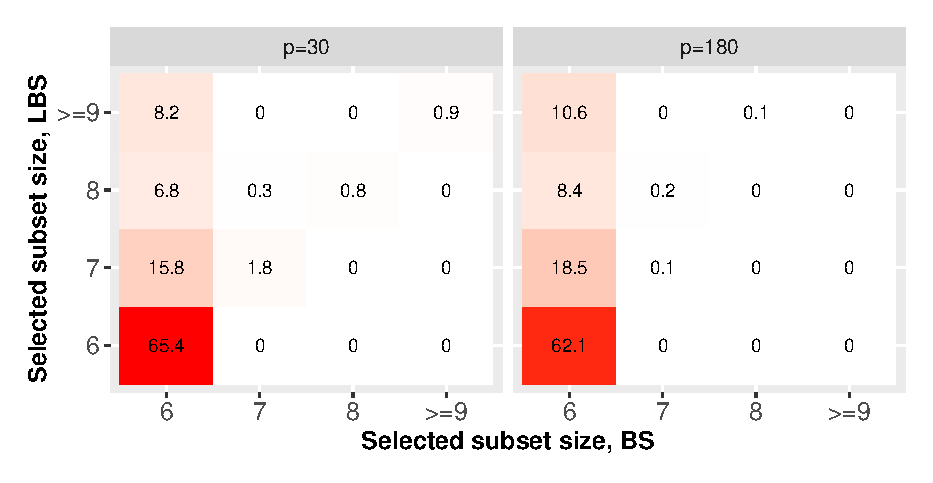
\includegraphics[width=0.9\textwidth]{figures/numvar_bs_lbs.eps}
	\caption{Frequency distributions (in $\%$) of the selected subset size  given by BS and LBS, based on $1000$ replications. The selection rule is C$_p$-edf. The true model is Orth-Sparse-Ex1 with $n=200$, $p_0=6$ and high SNR.}
	\label{fig:numvar_bs_lbs} 
\end{figure}


\iffalse
\begin{figure}[!ht]
	\centering
	\includegraphics[width=0.8\textwidth]{figures/lbs_bs_cp_eg.eps}
	\caption{C$_p$-edf at subset size $k$ for BS and LBS. The true model is Orth-Sparse-Ex1 with $n=200$, $p=180$, $p_0=6$ and high SNR. We assume knowledge of $\mu$ and $\sigma$.}
	\label{fig:lbs_bs_cp_eg} 
\end{figure}
\fi

%!TEX root = ms.tex
\section{Best orthogonalized subset selection (BOSS)}
\label{sec:boss}
With a general $X$, BS is not computationally feasible for large problems. In this section, we propose a LS-based subset selection method BOSS that has computational cost of the same order as a multiple regression on all of the predictors. 

\subsection{The method and its computational cost}
\label{sec:boss_alg}
The detailed implementation process of BOSS is described in Algorithm \ref{alg:boss}. The main steps can be summarized as follows: 1) order and orthogonalize the predictors, 2) perform BS on the set of orthogonal predictors, 3) transform the coefficients back to the original space, and 4) use a selection rule such as AICc-hdf to choose the single subset.

% main algorithm
\begin{algorithm}
	\caption{Best Orthogonalized Subset Selection (BOSS)}\label{alg:boss}
	\begin{enumerate}[label=\arabic*.]
		\item Standardize $y$ and the columns of $X$ to have mean $0$, and denote the means as $\bar{X}$ and $\bar{y}$.
		%\item Denote $S_k$ as the set of predictors that are active at step $k$ and let $S={1,\cdots, p}$.

		\textbf{Order and orthogonalize the predictors:}

		\item From the $p$ predictors, select the one that has the largest marginal correlation with the response $y$,  and denote it as $X_{S_1}$. Standardize $X_{S_1}$ to have unit $l_2$ norm and denote it as $Q_{S_1}$. Calculate $R_{S_1}$ such that $X_{S_1} = Q_{S_1} R_{S_1}$. Let $S=\{1,\cdots, p\}$. Initialize vectors $\text{resid}_j=X_j$ where $j=1,\cdots,p$.
		\item For $k=2,\cdots,p$:
		\begin{enumerate}[label=\alph*.]
			\item For each of the $p-k+1$ predictors $X_j$ in $X_{S \setminus S_{k-1} }$, calculate its partial correlations with the response $y$ conditioning on $Q_{S_{k-1}}$. 
			\iffalse
			\begin{enumerate}[label=a\arabic*.]
				\item Regress $y$ on $q$, augment $Z$ with the coefficient $z$. Set $\text{resid1} = \text{resid1} - zq$.
			\end{enumerate}
			\fi
			%\begin{enumerate}[resume*,label=a\arabic*.]
			\begin{enumerate}[label=a\arabic*.]
				%\item Regress $x_j$ on $q$, call the coefficient $r$. Set $\text{resid2}_j = \text{resid2}_j - rq$.
				%\item Calculate the correlation between resid1 and $\text{resid2}_j$.
				\item Regress $X_j$ on $Q_{S_{k-1} \setminus S_{k-2}}$ ($S_{k-2}=\emptyset$ if $k=2$), and denote the estimated coefficient as $r$. Update $\text{resid}_j = \text{resid}_j - r Q_{S_{k-1} \setminus S_{k-2}}$.
				\item Calculate the correlation between y and $\text{resid}_j$.
			\end{enumerate}
			\item Select the predictor that has the largest partial correlation in magnitude, augment $S_{k-1}$ with this predictor and call it $S_{k}$.
			\item Update $Q_{S_{k-1}}$ and $R_{S_{k-1}}$ given the newly added column $X_{S_k \setminus S_{k-1}}$, and call them $Q_{S_k}$ and $R_{S_k}$. The update is based on the modified Gram-Schmidt algorithm as discussed in \citet{hammarling2008updating}.
		\end{enumerate}
		
		\textbf{BS on the orthogonalized predictors $Q_{S_{p}}$:}

		\item Calculate $\tilde{\gamma}_j (k_Q)= z_j \mathbbm{1}(|z_j| \ge |z_{(k_Q)}|)$, i.e. the $j$-th component of coefficient vector for subset size $k_Q$, where $z=Q_{S_p}^T y$ and $z_{(k_Q)}$ is the $k$-th largest entry in absolute values. Let $\tilde{\gamma} = [\tilde{\gamma} (0) \tilde{\gamma} (1) \cdots \tilde{\gamma} (p)]$.
		
		\textbf{Transform back to the original space:}

		\item Project $\tilde{\gamma}$, a $p \times (p+1)$ matrix, to the original space of $X_{S_p}$, i.e. back solving $R \tilde{B} = \tilde{\gamma}$, and re-order the rows of $\tilde{B}$ to their correspondences in $X$, i.e. $\hat{B} = O \tilde{B}$ where $O$ represents the ordering matrix s.t. $X_{S_p}=XO$. The intercept vector is $\hat{B}_0 = \bar{y} \mathbbm{1} - \hat{B}^T \bar{X}$. 

		\textbf{Select the subset:}

		\item Select the subset using AICc-hdf, where hdf is calculated via Algorithm \ref{alg:hdf}, by inputting $(Q_{S_p},y)$. The inclusion of an intercept term implies that hdf$(k_Q)$ is increased by $1$.
	\end{enumerate}
\end{algorithm}


As can be seen in what follows, the computation of BOSS has an overall cost of $O(np^2)$, the same cost as OLS on all $p$ predictors and lasso. For step $k$, we have a set of ordered predictors $X_{S_{k-1}}$ and its orthogonal basis $Q_{S_{k-1}}$. From the remaining $p-k+1$ predictors, we choose the one that has the largest correlation with $y$ conditioning on $Q_{S_{k-1}}$, that is the correlation between $y$ and the residual from regressing a candidate predictor on $Q_{S_{k-1}}$. The regression part costs $O(n)$ since we maintain the regression result, e.g. estimated coefficients and residual, in the previous steps, and only need to perform a simple linear regression upon the predictor joined in step $k-1$, i.e. the last column in $Q_{S_{k-1}}$. Repeating the above step for all $p-k+1$ predictors costs $O(n(p-k+1))$. We then update the QR decomposition, by adding the chosen predictor as a new column, which costs $O(n(p-k))$ via the modified Gram-Schmidt algorithm as discussed in \citet{hammarling2008updating}. Therefore, we end up with an ordered set of predictors $X_{S_p}$ and its corresponding QR decomposition $Q_{S_p}$ and $R_{S_p}$. We regress $y$ upon $Q_{S_p}$ which costs $O(np)$, and denote the coefficient vector as $z$. BOSS then performs BS on $Q_{S_p}$, which is a ranking of predictors based on their magnitudes of corresponding element in $z$, and the cost is $O(p\log(p))$. Once we have the solution path of BOSS, we then apply AICc-hdf to choose the single subset size (denoted as $k_Q$), where hdf is calculated via Algorithm \ref{alg:hdf} by inputting $Q_{S_p}$. The entire BOSS-AICc-hdf procedure costs $O(np^2)$. 

The ordering of predictors is essential in terms of both getting a sparse solution and a better predictive performance. Consider a sparse true model with only two uncorrelated predictors $X=[X_1,X_2]$, $\beta=[0,1]^T$ and a high SNR. Based on the evidence we see from the previous section, the best model in such a scenario is LS regression on $X_2$. Without the ordering step, the orthogonal basis is $Q=[Q_1,Q_2]$ s.t. $X=QR$, i.e. the predictors are orthogonalized in their physical orders. The one-predictor model ($k_Q=1$) of BS can either be $Q_1$ or $Q_2$, which when transformed back to the space of $X$ do not correspond to LS regression upon $X_2$. The former corresponds to LS estimates upon $X_1$, while the latter is a linear combination of LS estimates upon $X$ and LS estimates upon $X_1$; the former leads to a completely wrong model while the latter results in non-zero coefficients on both predictors. In contrast, if $X_2$ is the first variable orthogonalized, the best subset will be based on that variable alone, the correct choice. Therefore, the ordering step is crucial to both sparsity as well as predictive performance. Note that we show the coefficients of BOSS can be expressed as a linear combination of LS coefficients on subsets of $X$ in Theorem \ref{thm:correspondence} and the proof can be found in the Supplemental Material. 

BS on the set of orthogonalized predictors gives the chance for BOSS to ``look back'' at the predictors that are already stepped in. One may notice that BOSS is similar to forward stepwise regression (FS), which was first introduced in \citet{efroymson1960multiple}. FS orders and orthogonalizes the predictors in the same way as BOSS. It then takes the nested subsets $Q_{S_1}, Q_{S_2}, \cdots, Q_{S_p}$ as the candidate subsets and performs LS regression upon them. Therefore, once a predictor is stepped in, it remains in the subsets of every following step of FS. As we will show in the next section, under certain circumstances, FS can easily overfit, since noise predictors (those with $\beta_j=0$) step in during early steps. However, BOSS revisits the predictors that have already stepped in and allows them to be dropped, resulting in a better predictive performance than FS.

\begin{theorem}[Coefficients of BOSS are a linear combination of LS coefficients on subsets of $X$] 
	Suppose $X$ has full column rank and the columns are already ordered. $X=QR$ where $Q$ is an $n \times p$ matrix with orthonormal columns and $R$ is a $p \times p$ upper-triangular matrix. Let $S_k=\{j_1,j_2,\cdots,j_{k_Q}\}$ denote the support (position of predictors) of the best $k_Q$-predictor model given by BS upon $(Q,y)$, and use $\hat{\gamma}(k_Q)$ ($p$ by $1$) to denote the BS coefficients. The corresponding coefficients in the $X$ space, i.e. $\hat{\beta}(k_Q)$ s.t. $R\hat{\beta}(k_Q)=\hat{\gamma}(k_Q)$, can be expressed as
	\begin{equation*}
	\hat{\beta}(k_Q) = \sum_{j\in S_k} \left(\hat{\alpha}^{(j)} - \hat{\alpha}^{(j-1)}\right),
	\end{equation*}
	where the first $j$ entries in $\hat{\alpha}^{(j)}$ ($p$ by $1$) are LS coefficients of regressing $y$ upon $[X_1,X_2,\cdots,X_j]$ (the first $j$ columns in $X$), and the remaining $p-j$ entries are zero.

	\label{thm:correspondence}
\end{theorem}

\subsection{Numerical justification of using hdf for BOSS}
The hdf is designed for BS on a set of orthogonal predictors. However, before performing BS on the orthogonal basis, BOSS first orders the predictors. This raises the question as to whether hdf is reasonable to use in the selection rules for BOSS. 

Figure \ref{fig:boss_cp_edf_hdf} compares averages of C$_p$-edf and C$_p$-hdf over $1000$ replications for BOSS under various true models. The details of setups for the sparse and dense models can be found in Section \ref{sec:simulation_setup_generalx}, where they correspond to the Sparse-Ex3 and Dense designs, respectively. The correlation between predictors is $\rho=0.5$. We see that by using the sample average to represent the population mean, $E(\text{C}_p\text{-hdf})$ approximates $E(\text{C}_p\text{-edf})$ well in most cases where the latter is also the expected prediction error $E(\text{Err}_\text{SE})$ by definition, and they converge as $k_Q$ approaches $p$. Moreover, both C$_p$-edf and C$_p$-hdf lead to the same average selected subset size, supporting the use of hdf in model selection for BOSS. 

Note that for any general fitting procedure including BOSS, C$_p$ provides an unbiased estimator of the testing error, and for that reason it is used in our discussions about the best-case performance when $\sigma$ is assumed to be known. Unfortunately, as discussed in Section \ref{sec:bs_ic_simulationresults}, using C$_p$ as the selection rule for BS can perform poorly in practice because of the need to estimate $\sigma$, particularly when $p$ is close to $n$. A similar property of using C$_p$ as the selection rule for BOSS will be shown in Section \ref{sec:boss_regu}. Therefore we prefer AICc in feasible versions of selection since it can perform considerably better. 

% {fig:boss_cp_edf_hdf}
\begin{figure}[ht!]
	\centering
	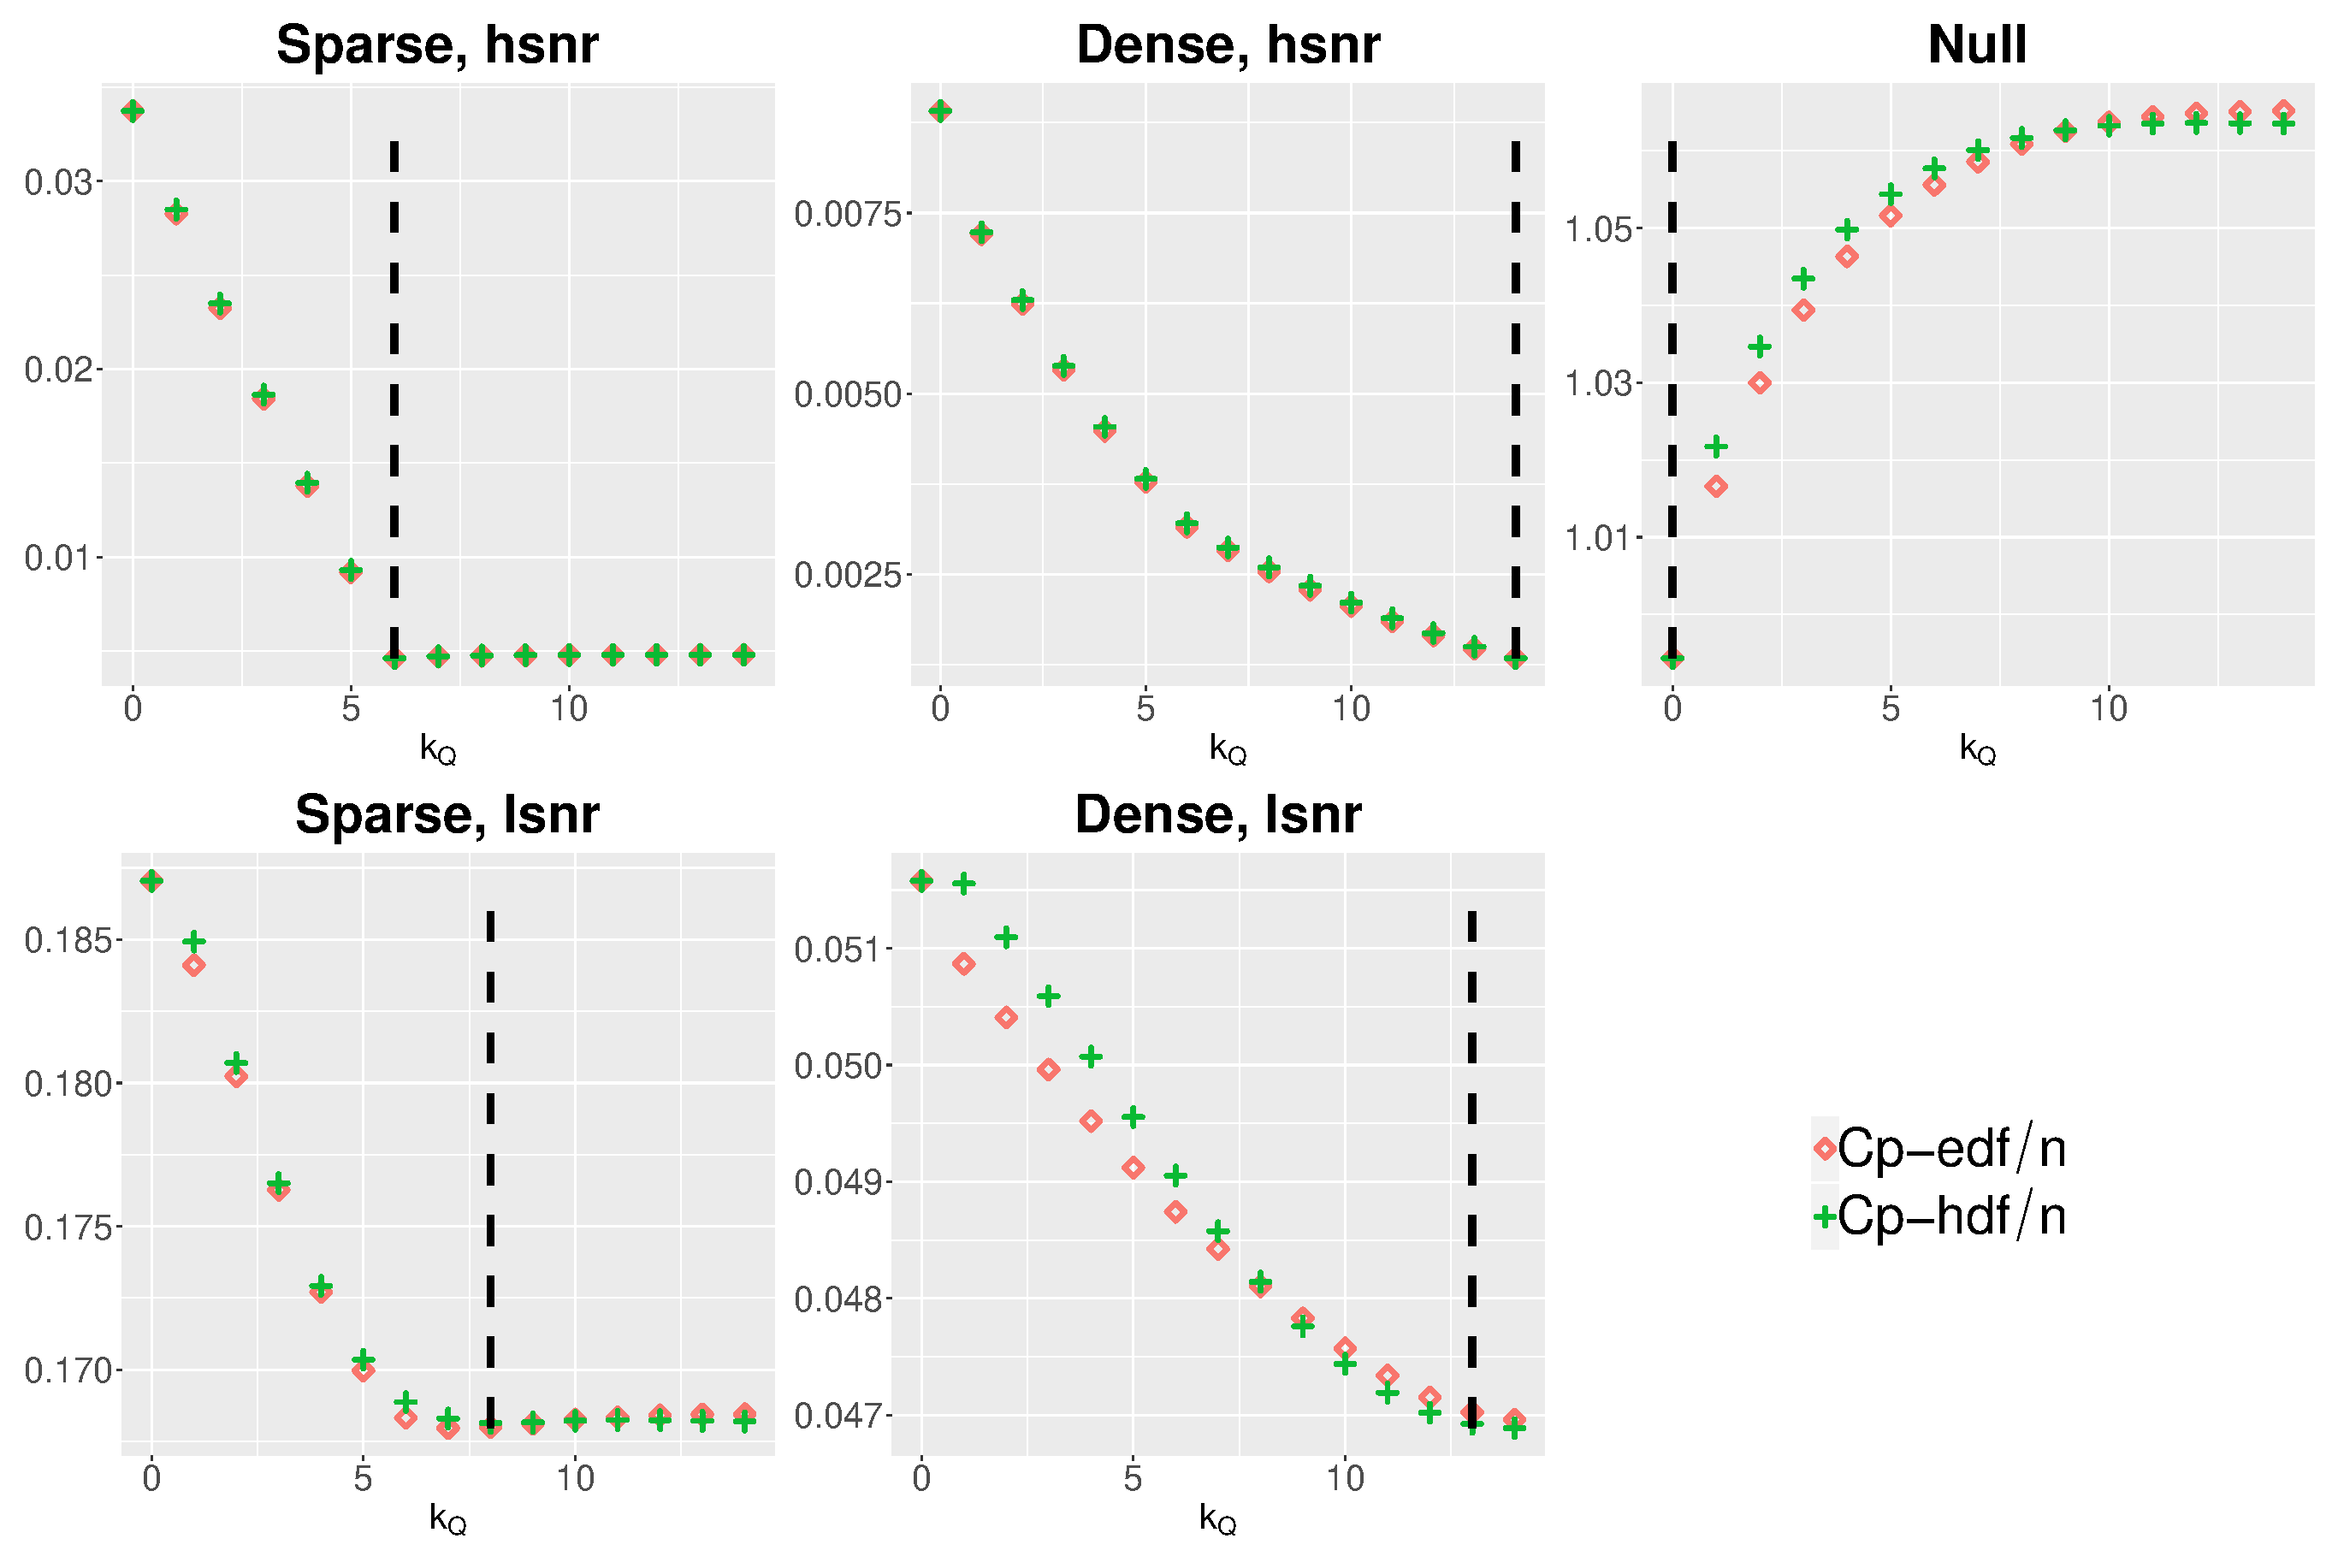
\includegraphics[width=0.9\textwidth]{figures/cp_edf_hdf_boss.eps}
	\caption{Averages of C$_p$-edf and C$_p$-hdf for BOSS over $1000$ replications. Here $X$ is general with $n=200$, $p=14$. Both criteria result in the same average of the selected subset size over the $1000$ replications (rounded to the nearest integer) as denoted by the dashed vertical lines. We assume knowledge of $\mu$ and $\sigma$.}
	\label{fig:boss_cp_edf_hdf}
\end{figure}

\subsection{The performance of BOSS}
We now study the performance of BOSS via simulations. We first show that BOSS can provide a better solution path than FS, and we further compare BOSS with regularization methods. 

\subsubsection{Simulation setups}
\label{sec:simulation_setup_generalx}
We consider a similar setup as in Section \ref{sec:simulation_setup_orthx}, but with a general $X$, where  $x_i\sim \mathcal{N}(0,\Sigma)$, $i=1,\cdots,n$ are independent realizations from a $p$-dimensional multivariate normal distribution with mean zero and covariance matrix $\Sigma=(\sigma_{ij})$. 

The correlation structure and true coefficient vector $\beta$ include the following scenarios:
\begin{itemize}
	\item Sparse-Ex1: \textbf{All of the predictors (both signal and noise) are correlated.} We take $\sigma_{i,j}=\rho^{|i-j|}$ for $i,j\in\{1,\cdots,p\}\times\{1,\cdots,p\}$. As to $\beta$, we have $\beta_j=1$ for $p_0$ equispaced values and $0$ everywhere else. 
	\item Sparse-Ex2: \textbf{Signal predictors are pairwise correlated with opposite effects.} We take $\sigma_{i,j}=\sigma_{j,i}=\rho$ for $1\le i <j \le p_0$. Other off-diagonal elements in $\Sigma$ are zero. For the true coefficient vector, we have $\beta_{2j-1}=1$ and $\beta_{2j}=-1$ for $1\le j \le p_0/2$, and all other $\beta_j=0$ for $j=p_0+1,\cdots,p$.
	\item Sparse-Ex3: \textbf{Signal predictors are pairwise correlated with noise predictors.} We take $\sigma_{i,j}=\sigma_{j,i}=\rho$ for $1\le i \le p_0$ and $j=p_0+i$. Other off-diagonal elements in $\Sigma$ are zero. $\beta=[1_{p_0},0_{p-p_0}]^T$.
	\item Sparse-Ex4: \textbf{Same correlation structure as Sparse-Ex2, but with varying strengths of coefficients.} We have $\beta_j=-\beta_{j+1}$ where $j=2k+1$ and $k=0,1,\cdots,p_0/2-1$. Suppose that $\beta^\prime=[1,5,10]$, then $\beta_j=\beta^\prime_k$ where $k=j (\text{mod} 3)$. 
	\item Dense: \textbf{Same correlation structure as Ex1, but with diminishing strengths of coefficients}. The true coefficient vector has: $\beta_j = \displaystyle (-1)^j \exp(-\frac{j}{\kappa})$, $j=1,\cdots,p$, and here $\kappa=10$.
	%\item Dense-Ex2: \textbf{Same setup as Dense-Ex1, but with slower decay}. Here we take $\kappa=50$.
\end{itemize}
The setup of Sparse-Ex1 is very common in the literature, such as in \citet{Bertsimas2016} and \citet{Hastie2017}. All of the predictors are correlated (when $\rho \ne 0$) where the strength of correlation depends on the physical positions of variables. Sparse-Ex2 is designed such that the pair of correlated predictors, e.g. $(X_1,X_2)$, leads to a good fit (high $R^2$), while either single one of them contribute little to the fitted $R^2$. Sparse-Ex4 is similar to Sparse-Ex2, but has varying strengths of coefficients for the true predictors. In Sparse-Ex3, signal predictors are only correlated with the noise ones. Finally, the dense setup is built on the dense example in Section \ref{sec:simulation_setup_orthx}, by having correlated predictors.

For the sparse examples, we take $p_0=6$. We consider three values of the correlation parameter, $\rho \in [0, 0.5, 0.9]$. Other configuration options, including $n$, $p$, and SNR, are the same as in Section \ref{sec:simulation_setup_orthx}. This implies a total of $360$ different combinations of configuration options. For each configuration, $1000$ replications are estimated and we present the same evaluation measures as introduced in Section \ref{sec:simulation_setup_orthx}. The full set of results can be found in the Supplemental Material.


\subsubsection{The solution paths of BOSS and FS}
Unlike FS, whose candidate subsets are nested, BOSS performs an extra step of BS upon $Q_{S_p}$, which raises the question of whether the extra step brings any benefit. We set aside the selection rule for now, and focus on the solution paths of the two methods. 

Figure \ref{fig:lossratio_fs_boss_k} shows two examples of the average RMSE along the solution paths of BS, FS and BOSS. When the true model is Sparse-Ex3, all three methods provide almost the same solution path. However, for Sparse-Ex4, we see a clear advantage of BOSS over FS in early steps up until about the fifteenth step. Recall that in Sparse-Ex4, there are $p_0=6$ predictors with $\beta_j \ne 0$ that are pairwise correlated with opposite effects, where each pair say $(X_1,X_2)$ together leads to a high $R^2$ but each single one of them ($X_1$ or $X_2$) contributes little. When the correlation between $X_1$ and $X_2$ is high, the effect of $X_1$ almost completely cancels out the effect of $X_2$ on $y$. Therefore all of predictors (both true and noise predictors) have approximately zero marginal correlation with $y$, and they have equal chance of stepping in. Since the subsets along the solution path of FS are nested, if a noise predictor steps in during early steps, it remains in the subsets of every following step, and hence the subset containing both $X_1$ and $X_2$ may appear in a late stage. In contrast, BOSS takes ordered predictors provided by FS, and re-orders them by performing BS upon their orthogonal basis, which gives a greater chance for $(X_1,X_2)$ to appear early in the solution path of BOSS and potentially results in a better predictive performance than FS. Furthermore, in this example, we notice that BOSS provides a better solution path than BS until step $5$ (except the fourth step), and the two methods give similar performances in further steps.

% {fig:lossratio_fs_boss_k}
\begin{figure}[ht!]
	\centering
	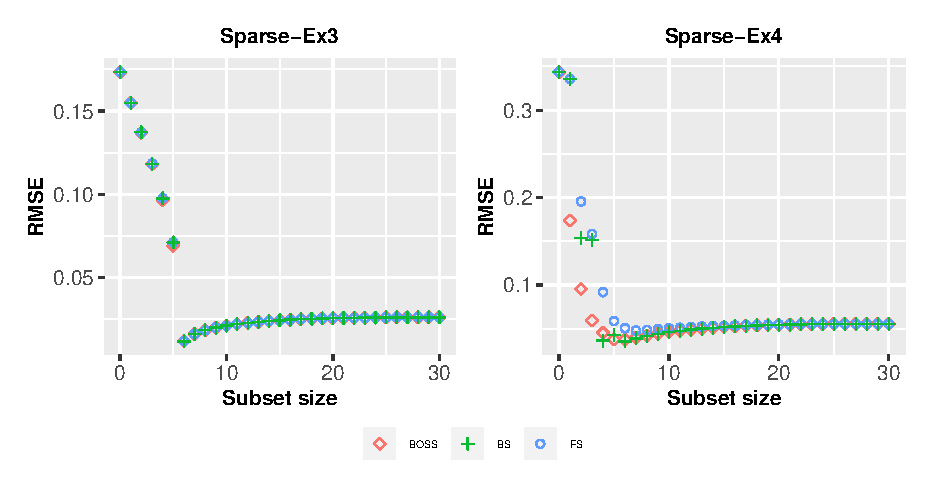
\includegraphics[width=\textwidth]{figures/rmse_solpath_lsmethods.eps}
	\caption{RMSE at each subset size, average over $1000$ replications. Note that for BOSS, the subset size $k_Q$ denotes the number of non-zero coefficients in $\hat{\gamma}(k_Q)$. In both scenarios, we have $n=200$, $p=30$, $\rho=0.9$ and high SNR.}
	\label{fig:lossratio_fs_boss_k}
\end{figure}


\subsubsection{The performance of BOSS compared to other methods}
\label{sec:boss_regu}
We now consider feasible implementations of the estimation methods. We looked at results using AICc-hdf, C$_p$-hdf and 10-fold CV for BOSS, and AICc-hdf was the best (see Supplemental Material), so that is what we will use here. For BS and FS, we will use 10-fold CV. Similar to our discussion in Section \ref{sec:bs_regu}, we find that (see Supplemental Material) AICc performs similarly to 10-fold CV for lasso, and that is what we will use for lasso. For other regularization methods, the selection rule will be 10-fold CV. According to our results (see Supplemental Material), SparseNet is slightly better than relaxed lasso and gamma lasso, and therefore we only present the results for SparseNet here. 

A selected set of simulation results is presented in Table \ref{tab:boss_regu}. Note that for BS, we only have results for $p\le 30$, since it is fitted using the ``leaps'' algorithm and $p \approx 30$ is the ad-hoc limit. We present the results in terms of $\%$ worse than the best possible BOSS, where the best possible BOSS means that on a single fit, we choose the subset size $k_Q$ with the minimum RMSE among all $p+1$ candidates, as if an oracle tells us the true model. Here is a brief summary of the results:


\begin{itemize}
	\item For BOSS, AICc-hdf has a significant advantage over CV in terms of predictive performance, except for $n=200$ and low SNR, in which case both selection rules are comparable. CV is also ten times heavier in terms of computation than AICc-hdf. These results are similar to the comparison of AICc-hdf and CV for BS with an orthogonal $X$ as discussed in Section \ref{sec:bs_ic_simulationresults}. Overall, the simulations indicate that AICc with hdf used in place of edf is a reasonable selection rule for an LS-based method that can be applied in practice without the requirement that the predictors are orthogonal. In the following discussions, when we refer to BOSS, we mean BOSS-AICc-hdf. 

	\item The performance of BOSS is comparable to the performance of BS when BS is feasible. With a small sample size $n=200$, BOSS performs either similarly to or better than BS for a high SNR, and it performs either similarly to or slightly worse than BS for a low SNR. With a large sample size $n=2000$, BOSS is generally better than BS. Furthermore, BOSS only requires fitting the procedure once while BS uses CV as the selection rule, and a single fit of BOSS only has computational cost $O(np^2)$ so that BOSS is feasible for high dimensions.

	\item The performance of BOSS is generally better than the performance of FS. In the Dense model, and Sparse-Ex3 with $n=200$ and low SNR, we see that BOSS performs similarly to FS. In all other scenarios, the advantage of BOSS is obvious. For example, in Sparse-Ex4 with $n=200$, high SNR and $\rho=0.9$, FS is almost ten times worse than BOSS in terms of RMSE. Recall that Sparse-Ex4 is an example where FS has trouble stepping in all of the true predictors (with $\beta_j \ne 0$) in early steps. This is evidenced by the fact that FS chooses eight extra predictors on average in this situation, while BOSS only chooses approximately two extra predictors. Furthermore, FS based on CV is ten times computationally heavier than BOSS. 

	\item Compared to the regularization methods, with a small sample size $n=200$, BOSS is the best when SNR is high, lasso is the best when SNR is low and SparseNet is in between. With $n=2000$, BOSS is almost always the best even when SNR is low. These findings are consistent with the discussion in Section \ref{sec:bs_regu}, where we compare the performance of BS with regularization methods under an orthogonal $X$. 

	\item In terms of support recovery in the sparse true models, LS-based methods can recover the true predictors (those with $\beta_j \ne 0$) and rarely include any noise predictors (those with $\beta_j = 0$) when SNR is high or the sample size $n$ is large. However, SparseNet and lasso generally overfit, with the latter being worse in that regard. In the low SNR and small $n$ scenario, lasso and SparseNet have more opportunity to recover the true predictors, but it comes with a price of including more false positives. 

\end{itemize}


% tab:boss_regu
% latex table generated in R 3.6.1 by xtable 1.8-4 package
% Sat Nov  9 17:57:42 2019
\begin{table}[ht]
\centering
\caption{The performance of BOSS compared to other methods for $n>p$. Selection rules are 'AICc-hdf/CV' for BOSS, 
                AICc for lasso and CV for the remaining methods in the table, respectively.} 
\label{tab:boss_regu}
\scalebox{0.5}{
\begin{tabular}{|c|c|c|c|ccccc|ccccc|ccccc|}
  \toprule 
 \multicolumn{1}{|r}{} & \multicolumn{1}{r}{} & \multicolumn{1}{r}{} &       & \multicolumn{5}{c|}{Sprse-Ex3}        & \multicolumn{5}{c|}{Sparse-Ex4}       & \multicolumn{5}{c|}{Dense} \\
 \cmidrule{5-19}\multicolumn{1}{|r}{} & \multicolumn{1}{r}{} & \multicolumn{1}{r}{} &       & BOSS  & BS    & FS    & lasso & SparseNet & BOSS  & BS    & FS    & lasso & SparseNet & BOSS  & BS    & FS    & lasso & \multicolumn{1}{c|}{SparseNet}  \\
 \cmidrule{5-19}\multicolumn{1}{|c}{} & \multicolumn{1}{c}{} & \multicolumn{1}{c}{} &       & \multicolumn{15}{c|}{\% worse than the best possible BOSS}  \\
 \midrule 
 \multirow{8}[4]{*}{n=200} & \multirow{4}[2]{*}{hsnr} & \multirow{2}[1]{*}{$\rho=0.5$} & p=30 & 2/22 & 24 & 22 & 70 & 14 & 19/24 & 23 & 28 & 49 & 21 & 1/8 & 9 & 8 & 2 & 5 \\ 
   &  &  & p=180 & 1/18 & - & 21 & 135 & 17 & 4/15 & - & 16 & 82 & 13 & 14/13 & - & 16 & 47 & 8 \\ 
   &  & \multirow{2}[1]{*}{$\rho=0.9$} & p=30 & 5/41 & 17 & 41 & 66 & 12 & 21/33 & 21 & 56 & 73 & 28 & 2/9 & 10 & 8 & 2 & 8 \\ 
   &  &  & p=180 & 3/27 & - & 29 & 126 & 16 & 7/34 & - & 68 & 123 & -10 & 15/12 & - & 12 & 71 & 20 \\ 
  \cmidrule{2-19} & \multirow{4}[2]{*}{lsnr} & \multirow{2}[1]{*}{$\rho=0.5$} & p=30 & 30/25 & 25 & 25 & 0 & 7 & 35/32 & 23 & 34 & 35 & 23 & 18/17 & 16 & 18 & 10 & 11 \\ 
   &  &  & p=180 & 11/13 & - & 13 & -3 & 3 & 31/26 & - & 34 & 33 & 20 & 4/8 & - & 9 & 2 & 6 \\ 
   &  & \multirow{2}[1]{*}{$\rho=0.9$} & p=30 & 28/24 & 23 & 23 & -2 & 5 & 32/27 & 18 & 78 & 71 & 44 & 15/14 & 15 & 13 & 10 & 12 \\ 
   &  &  & p=180 & 16/16 & - & 15 & -5 & 1 & 17/18 & - & 36 & 33 & 35 & 12/10 & - & 10 & 15 & 9 \\ 
  \midrule \multirow{8}[4]{*}{n=2000} & \multirow{4}[2]{*}{hsnr} & \multirow{2}[1]{*}{$\rho=0.5$} & p=30 & 3/22 & 22 & 21 & 73 & 14 & 7/29 & 21 & 23 & 86 & 12 & 0/3 & 0 & 0 & 1 & 0 \\ 
   &  &  & p=180 & 1/22 & - & 22 & 130 & 14 & 6/28 & - & 21 & 174 & 12 & 8/9 & - & 12 & 37 & 8 \\ 
   &  & \multirow{2}[1]{*}{$\rho=0.9$} & p=30 & 2/21 & 21 & 22 & 74 & 13 & 32/33 & 16 & 33 & 108 & 12 & 0/3 & 1 & 1 & 2 & 1 \\ 
   &  &  & p=180 & 1/21 & - & 22 & 135 & 14 & 15/25 & - & 90 & 226 & 10 & 10/10 & - & 9 & 39 & 17 \\ 
  \cmidrule{2-19} & \multirow{4}[2]{*}{lsnr} & \multirow{2}[1]{*}{$\rho=0.5$} & p=30 & 5/22 & 21 & 21 & 73 & 14 & 13/30 & 22 & 23 & 61 & 15 & 2/9 & 10 & 10 & 2 & 7 \\ 
   &  &  & p=180 & 5/22 & - & 22 & 129 & 13 & 8/27 & - & 20 & 125 & 10 & 11/13 & - & 16 & 32 & 10 \\ 
   &  & \multirow{2}[1]{*}{$\rho=0.9$} & p=30 & 5/21 & 20 & 21 & 53 & 3 & 27/34 & 16 & 40 & 85 & 12 & 3/11 & 11 & 9 & 3 & 8 \\ 
   &  &  & p=180 & 4/17 & - & 17 & 92 & -5 & 14/27 & - & 104 & 179 & 20 & 12/13 & - & 11 & 40 & 18 \\ 
   \midrule 
 \multicolumn{1}{|c}{} & \multicolumn{1}{c}{} & \multicolumn{1}{c}{} &       & \multicolumn{15}{c|}{Relative efficiency} \\
 \midrule 
\multirow{8}[4]{*}{n=200} & \multirow{4}[2]{*}{hsnr} & \multirow{2}[1]{*}{$\rho=0.5$} & p=30 & 1/0.84 & 0.82 & 0.84 & 0.6 & 0.9 & 1/0.96 & 0.97 & 0.93 & 0.8 & 0.99 & 0.98/0.93 & 0.91 & 0.93 & 0.98 & 0.94 \\ 
   &  &  & p=180 & 1/0.85 & - & 0.84 & 0.43 & 0.86 & 1/0.91 & - & 0.9 & 0.57 & 0.92 & 0.95/0.96 & - & 0.93 & 0.73 & 1 \\ 
   &  & \multirow{2}[1]{*}{$\rho=0.9$} & p=30 & 1/0.74 & 0.9 & 0.74 & 0.63 & 0.93 & 1/0.91 & 1 & 0.78 & 0.7 & 0.95 & 0.98/0.91 & 0.9 & 0.92 & 0.98 & 0.93 \\ 
   &  &  & p=180 & 1/0.8 & - & 0.79 & 0.45 & 0.88 & 0.84/0.68 & - & 0.54 & 0.41 & 1 & 0.97/1 & - & 1 & 0.65 & 0.93 \\ 
  \cmidrule{2-19} & \multirow{4}[2]{*}{lsnr} & \multirow{2}[1]{*}{$\rho=0.5$} & p=30 & 0.77/0.8 & 0.8 & 0.8 & 1 & 0.93 & 0.91/0.93 & 1 & 0.92 & 0.91 & 1 & 0.93/0.94 & 0.95 & 0.93 & 1 & 0.99 \\ 
   &  &  & p=180 & 0.87/0.86 & - & 0.86 & 1 & 0.94 & 0.92/0.96 & - & 0.9 & 0.91 & 1 & 0.97/0.94 & - & 0.94 & 1 & 0.96 \\ 
   &  & \multirow{2}[1]{*}{$\rho=0.9$} & p=30 & 0.76/0.79 & 0.8 & 0.8 & 1 & 0.93 & 0.89/0.93 & 1 & 0.66 & 0.69 & 0.82 & 0.96/0.97 & 0.96 & 0.97 & 1 & 0.98 \\ 
   &  &  & p=180 & 0.82/0.82 & - & 0.83 & 1 & 0.95 & 1/0.99 & - & 0.86 & 0.88 & 0.87 & 0.97/0.99 & - & 1 & 0.95 & 1 \\ 
  \midrule \multirow{8}[4]{*}{n=2000} & \multirow{4}[2]{*}{hsnr} & \multirow{2}[1]{*}{$\rho=0.5$} & p=30 & 1/0.85 & 0.85 & 0.85 & 0.59 & 0.91 & 1/0.83 & 0.89 & 0.87 & 0.58 & 0.96 & 0.98/0.96 & 0.98 & 0.98 & 0.97 & 0.98 \\ 
   &  &  & p=180 & 1/0.83 & - & 0.83 & 0.44 & 0.89 & 1/0.83 & - & 0.88 & 0.39 & 0.95 & 1/0.99 & - & 0.96 & 0.79 & 1 \\ 
   &  & \multirow{2}[1]{*}{$\rho=0.9$} & p=30 & 1/0.84 & 0.85 & 0.84 & 0.59 & 0.9 & 0.84/0.84 & 0.96 & 0.84 & 0.54 & 1 & 1/0.97 & 0.99 & 0.99 & 0.98 & 0.99 \\ 
   &  &  & p=180 & 1/0.84 & - & 0.83 & 0.43 & 0.89 & 0.96/0.88 & - & 0.58 & 0.34 & 1 & 0.99/0.99 & - & 1 & 0.78 & 0.93 \\ 
  \cmidrule{2-19} & \multirow{4}[2]{*}{lsnr} & \multirow{2}[1]{*}{$\rho=0.5$} & p=30 & 1/0.86 & 0.86 & 0.86 & 0.61 & 0.92 & 1/0.87 & 0.93 & 0.92 & 0.7 & 0.99 & 0.98/0.91 & 0.9 & 0.91 & 0.98 & 0.93 \\ 
   &  &  & p=180 & 1/0.86 & - & 0.86 & 0.46 & 0.93 & 1/0.85 & - & 0.9 & 0.48 & 0.98 & 1/0.97 & - & 0.95 & 0.83 & 1 \\ 
   &  & \multirow{2}[1]{*}{$\rho=0.9$} & p=30 & 0.98/0.85 & 0.86 & 0.85 & 0.67 & 1 & 0.88/0.83 & 0.97 & 0.8 & 0.61 & 1 & 1/0.92 & 0.92 & 0.94 & 1 & 0.95 \\ 
   &  &  & p=180 & 0.91/0.81 & - & 0.81 & 0.49 & 1 & 1/0.9 & - & 0.56 & 0.41 & 0.95 & 0.99/0.99 & - & 1 & 0.8 & 0.94 \\ 
   \midrule 
 \multicolumn{1}{|c}{} & \multicolumn{1}{c}{} & \multicolumn{1}{c}{} &       & \multicolumn{15}{c|}{Sparsistency (number of extra variables)} \\
 \midrule 
\multirow{8}[4]{*}{n=200} & \multirow{4}[2]{*}{hsnr} & \multirow{2}[1]{*}{$\rho=0.5$} & p=30 & 6(0)/6(0.6) & 6(0.7) & 6(0.6) & 6(7.9) & 6(1.1) & 4.4(0.2)/5(1) & 5(1) & 4.8(1.1) & 5.7(10.4) & 4.8(2.1) & 29.6/26.1 & 25.1 & 26 & 29.1 & 27 \\ 
   &  &  & p=180 & 6(0)/6(0.3) & - & 6(0.4) & 6(16.6) & 6(2.4) & 4(0)/4.2(0.5) & - & 4.1(0.5) & 5.1(20.2) & 4.2(3.5) & 17/20.2 & - & 19.6 & 52.2 & 32.4 \\ 
   &  & \multirow{2}[1]{*}{$\rho=0.9$} & p=30 & 6(0.6)/6(2.1) & 6(0.8) & 6(2.1) & 6(9.2) & 6(1.6) & 5.1(2.8)/5.3(3.8) & 5(1) & 4.8(4.1) & 5.8(17.8) & 4.4(2.7) & 29.3/25.2 & 23 & 24.6 & 28.9 & 26.2 \\ 
   &  &  & p=180 & 6(0.1)/6(0.6) & - & 6(0.6) & 6(16.2) & 6(2.4) & 4.2(2.4)/4.3(4.3) & - & 4.3(8) & 4.6(44.2) & 4.1(3.1) & 15.6/21.3 & - & 17.2 & 54.4 & 37.7 \\ 
  \cmidrule{2-19} & \multirow{4}[2]{*}{lsnr} & \multirow{2}[1]{*}{$\rho=0.5$} & p=30 & 2.9(2)/3.6(2.4) & 3.4(2.1) & 3.5(2.3) & 5.1(6.9) & 4.7(5.3) & 2.3(1)/2.7(1.3) & 2.6(1) & 2.6(1.5) & 3.6(6.9) & 2.8(2.9) & 5.7/7.5 & 6.6 & 7.1 & 5.3 & 10.3 \\ 
   &  &  & p=180 & 0.3(0.1)/1(0.7) & - & 1(0.7) & 3(9.7) & 2.6(9.3) & 1(0.2)/1.6(0.9) & - & 1.3(0.8) & 2.2(10.7) & 2.1(6.5) & 0.2/1.1 & - & 0.9 & 2.7 & 6.9 \\ 
   &  & \multirow{2}[1]{*}{$\rho=0.9$} & p=30 & 1.9(2.3)/2.4(3) & 2.5(2.8) & 2.4(2.9) & 3.9(7.5) & 3.7(6.1) & 2.7(3.9)/3.2(5) & 2.7(0.9) & 2.2(4.4) & 3(10.1) & 2.9(8) & 4.1/5.2 & 4.3 & 4.5 & 8.4 & 5.9 \\ 
   &  &  & p=180 & 0.5(0.2)/1.1(1.1) & - & 1.1(1.1) & 3.2(11.1) & 3(10.8) & 0.7(1.7)/1.1(5.5) & - & 0.2(0.6) & 0.3(4.8) & 0.6(9) & 1/2.1 & - & 1.6 & 3.9 & 3.3 \\ 
  \midrule \multirow{8}[4]{*}{n=2000} & \multirow{4}[2]{*}{hsnr} & \multirow{2}[1]{*}{$\rho=0.5$} & p=30 & 6(0.1)/6(0.6) & 6(0.6) & 6(0.6) & 6(8.4) & 6(1) & 6(0.2)/6(0.6) & 6(0.6) & 6(0.6) & 6(10.9) & 6(0.8) & 30/30 & 30 & 30 & 30 & 30 \\ 
   &  &  & p=180 & 6(0)/6(0.4) & - & 6(0.4) & 6(21.5) & 6(2.3) & 6(0.1)/6(0.3) & - & 6(0.3) & 6(32.2) & 6(1.3) & 34.5/35.1 & - & 32.6 & 106.5 & 43 \\ 
   &  & \multirow{2}[1]{*}{$\rho=0.9$} & p=30 & 6(0)/6(0.6) & 6(0.6) & 6(0.6) & 6(9.2) & 6(1) & 6(0.4)/6(0.7) & 6(0.6) & 6(1.3) & 6(17.8) & 6(1.6) & 30/29.9 & 29.9 & 29.9 & 30 & 30 \\ 
   &  &  & p=180 & 6(0)/6(0.4) & - & 6(0.4) & 6(23.2) & 6(2.2) & 6(1.4)/6(1.7) & - & 5.9(3.8) & 6(72.7) & 6(8.7) & 35/38.6 & - & 30.2 & 109.6 & 52.4 \\ 
  \cmidrule{2-19} & \multirow{4}[2]{*}{lsnr} & \multirow{2}[1]{*}{$\rho=0.5$} & p=30 & 6(0.1)/6(0.6) & 6(0.6) & 6(0.6) & 6(8.3) & 6(0.7) & 4.2(0.4)/4.3(0.7) & 4.3(0.6) & 4.2(0.7) & 5.2(9.6) & 4.3(1) & 29/22.7 & 21.2 & 22.1 & 28 & 24.1 \\ 
   &  &  & p=180 & 6(0.1)/6(0.4) & - & 6(0.4) & 6(21.2) & 6(0.9) & 4(0.1)/4(0.4) & - & 4(0.4) & 4.6(26.1) & 4.1(1.3) & 16/17 & - & 14.3 & 61.8 & 25.3 \\ 
   &  & \multirow{2}[1]{*}{$\rho=0.9$} & p=30 & 5.8(0.3)/5.8(1.1) & 5.8(1.1) & 5.8(1.1) & 6(9.2) & 6(0.8) & 4.4(1.9)/4.4(1.7) & 4.3(0.6) & 4.3(2.2) & 5.4(16.6) & 4.2(2.5) & 28.8/21.2 & 18.5 & 20.2 & 27.6 & 23.5 \\ 
   &  &  & p=180 & 5.7(0.3)/5.7(0.7) & - & 5.7(0.7) & 6(23) & 6(1) & 4.1(3.6)/4.1(4.4) & - & 3.7(3.7) & 4.6(60.3) & 4.2(14.2) & 16.6/21.4 & - & 11.8 & 65.3 & 32.3 \\ 
   \bottomrule 
\end{tabular}
}
\end{table}


 %!TEX root = boss.tex
\section{Real data analysis}
\label{sec:real_data}
In this section, we implement BOSS on five real world datasets. We consider four datasets from the StatLib library\footnote{http://lib.stat.cmu.edu/datasets/}, which is maintained at Carnegie Mellon University. The `Housing' data are often used in comparisons of different regression methods. The aim is to predict the housing values in the suburbs of Boston based on $13$ predictors, including crime rate, property tax rate, pupil-teacher ratio, etc. The `Hitters' data contain the 1987 annual salary for MLB players. For each player, it records $19$ different performance metrics happening in 1986, such as number of times at bat, number of hits, etc., and the task is to predict the salary based on these statistics. The `Auto' data are driven by prediction of the miles per gallon of vehicles based on features like the horsepower, weight, etc. The `College' data contain various statistics for a large number of US colleges from the 1995 issue of `US News and World Report', and we use these statistics to predict the number of applications received. We also consider a dataset from the Machine Learning Repository\footnote{https://archive.ics.uci.edu/ml} that is maintained by UC Irvine. The `ForestFire' data are provided by \citet{cortez2007data} and the aim is to use meteorological and other data to predict the burned area of forest fires that happened in the northeast region of Portugal. The authors considered several machine learning algorithms, e.g. support vector regression, and concluded that the best prediction in terms of RMSE is the naive mean vector.

%The 'AirFoil' data has different size airfoils at different wind tunnel speeds and angles of attack, based on experiments performed by NASA, and the purpose is to predict sound pressure level. 

In real data analysis, one almost always would consider an intercept term. The way that BOSS handles the intercept term is described in Algorithm \ref{alg:boss}. To be more specific, we first center both $X$ and $y$, and fit BOSS-AICc-hdf without an intercept to get $\hat{\beta}$. Then we calculate the intercept by $
\hat{\beta}_0=\bar{y} - \bar{X}^T \hat{\beta}$, which can be easily shown to be equivalent to fitting an intercept in every subset considered by BOSS. 

We compare the performance of BOSS with LS-based methods BS and FS, and with regularization methods LASSO and SparseNet. All of the methods are fitted with an intercept term. Note that for the Forest Fires dataset, we fit BS via MIO \citep{Bertsimas2016} using the {\tt{R}} package \pkg{bestsubset} \citep{Hastie2017}, where we restrict subset size $k=0,\dots,10$, with $3$ minutes as the time budget to find an optimal solution for each $k$, as suggested by the authors. For all of the other datasets, BS is fitted using the \pkg{leaps} package. To measure the performance of each method, we apply the leave-one-out (LOO) testing procedure, in which we fit the method on all observations except one, test the performance on that particular observation, and repeat the procedure for all $n$ observations. 

Table \ref{tab:realdata} presents the average RMSE, the average number of predictors and average running time for various methods given by LOO testing. We see that BOSS provides the best predictive performance in all datasets except the `Housing' and `College' data where LASSO is the best for those datasets and its RMSE is $0.3\%$ and $0.04\%$ lower than those of BOSS, respectively. Due to a highly optimized implementation of the cyclical coordinate descent, the `glmnet' algorithm is extremely fast to provide the LASSO solution. BS is still not scalable to large dimensions, even by using the modern tools. With the dimension $p=55$, it takes around $350$ seconds to perform 10-fold CV for subset sizes restricted to be no greater than $10$. However, We observe that BOSS is reasonably computationally efficient and much faster than BS, FS and SparseNet. 

% tab:realdata
% latex table generated in R 3.6.1 by xtable 1.8-4 package
% Sun Nov 10 11:56:55 2019
\begin{table}[ht]
\centering
\caption{Performance of subset selection methods on real datasets. 
               The results are averages of leave-one-out (LOO) testing. 
               The selection rules are AICc-hdf for BOSS, AICc for lasso and 10-fold CV for the rest, respectively. 
               The intercept term is always fitted and is not counted in the number of predictors. 
               Minimal values for the metrics for each dataset are given in bold face.} 
\label{tab:realdata}
\scalebox{0.9}{
\begin{tabular}{|c|c|ccc|c|c|}
  \toprule 
 Dataset (n, p) & Metrics & BOSS  & BS    & FS    & lasso & SparseNet  \\
 \midrule\multirow{3}[2]{*}{Housing (506, 13)} & RMSE & 3.372 & 3.37 & 3.383 & \textbf{3.363} & 3.369 \\ 
   & \# predictors & 12.004 & \textbf{12.002} & 12.026 & 12.012 & \textbf{12.002} \\ 
   & running time (s) & 0.021 & 0.066 & 0.156 & 0.007 & 0.39 \\ 
  \midrule\multirow{3}[2]{*}{Hitters (263, 19)} & RMSE & \textbf{233.853} & 236.989 & 238.222 & 234.064 & 238.375 \\ 
   & \# predictors & 11.152 & 10.852 & \textbf{10.662} & 14.205 & 12.51 \\ 
   & running time (s) & 0.014 & 0.095 & 0.104 & 0.008 & 0.493 \\ 
  \midrule \multirow{3}[2]{*}{Auto (392, 6)} & RMSE & \textbf{2.628} & \textbf{2.628} & \textbf{2.628} & 2.643 & 2.63 \\ 
   & \# predictors & \textbf{3} & 3.003 & \textbf{3} & 5.008 & 3.008 \\ 
   & running time (s) & 0.008 & 0.051 & 0.067 & 0.007 & 0.25 \\ 
  \midrule\multirow{3}[2]{*}{College (777, 17)} & RMSE & 1565.476 & 1568.234 & 1569.625 & \textbf{1564.807} & 1573.975 \\ 
   & \# predictors & 17.991 & 16.333 & 16.067 & 16.008 & \textbf{15.385} \\ 
   & running time (s) & 0.058 & 0.092 & 0.451 & 0.01 & 0.734 \\ 
  \midrule\multirow{3}[2]{*}{Forest Fires (517, 55)} & RMSE & \textbf{18.603} & 18.707 & 18.757 & 18.726 & 19.163 \\ 
   & \# predictors & \textbf{0} & 0.983 & 0.986 & 2.985 & 6.899 \\ 
   & running time (s) & 0.084 & 356.651 & 0.593 & 0.014 & 0.785 \\ 
   \bottomrule 
\end{tabular}
}
\end{table}





 %!TEX root = boss.tex
\section{CONCLUSION AND FUTURE WORK}
\label{sec:conclusion}
In this paper, we introduce a heuristic degrees of freedom (hdf) for BS based on an orthogonal $X$. We further propose a KL-based information criterion AICc-edf and its feasible implementation AICc-hdf. We show that their expected values can reasonably approximate the expected KL, $E(\text{Err}_\text{KL})$. Moreover, they result in the same choice of subset as $\widehat{\text{Err}}_{\text{KL}}$  when they are used as selection rules for BS. Furthermore, we propose an LS-based subset selection method BOSS. BOSS together with the selection rule AICc-hdf has computational cost on the same order as OLS. Finally, we show in simulations and real data examples that BOSS can be a competitive method in both speed and predictive performance. 

Since edf \eqref{eq:edf} for LS-based methods is saturated at $n$ when $p\ge n$, potential future work is to study a measure of complexity and build a connection with the use of information criteria in the case of $p \ge n$. The strong performance of BOSS using AICc compared to using CV suggests that the pursuit of methods to approximate edf (which normally does not have an analytical expression for complex modeling methods and algorithms), particularly for methods that are more sensitive to small perturbations in the data, is worthy of further research.

\clearpage
\bibliographystyle{chicago}
\bibliography{reference.bib}

%!TEX root = ms.tex
\beginsupplement
\appendix
\pagenumbering{arabic}
\begin{center}
\textbf{\large Supplementary Materials \\
On the Use of Information Criteria for Subset Selection \\ in Least Squares Regression}

Sen Tian, Clifford M. Hurvich, Jeffrey S. Simonoff
\end{center}

\section{Technical details}
\subsection{Proof of theorem \ref{thm:hdf_ydf_representation} and its corollary}
\label{sec:proof_hdf_ydf}
In this section, we assume an orthogonal $X$ and a null true model. This is the only scenario under which both df$_C(k)$ and hdf$(k)$ have analytical expressions. We will prove that the ratio of df$_C(k)$ and hdf$(k)$ goes to $1$ as $k,p\rightarrow \infty$ while $k=\left \lfloor{xp}\right \rfloor $, where $\left \lfloor{\cdot}\right \rfloor$ denotes the greatest integer function and $x\in(0,1)$. We start by laying out a few lemmas to be used in the proof of the main theorem.
\begin{lemma}
	\label{lemma:hdf_nulltrue}
	Assume the design matrix is orthogonal and the true model is null ($\mu=0$). Then
	\begin{equation}
	\text{hdf}(k) = df_L(\lambda_k^\star) = k - 2p\cdot \Phi^{-1} \left(\frac{k}{2p}\right) \cdot \phi\left[\Phi^{-1}\left(\frac{k}{2p}\right) \right].
	\label{eq:hdf_nulltrue}
	\end{equation}
\end{lemma}
\begin{proof}
	We follow the steps described in algorithm \ref{alg:hdf}. We first find $\lambda_k^\star$ from \eqref{eq:thdf_size_expression}, by using the fact that $\mu=0$, and we get $\displaystyle -\frac{\sqrt{2\lambda_k^\star}}{\sigma} = \displaystyle \Phi^{-1}\left(\frac{k}{2p}\right)$, which we then substituted into \eqref{eq:thdf_expression} to get \eqref{eq:hdf_nulltrue}.
\end{proof}

\iffalse
\begin{lemma}
	\label{lemma:hdf_limitends}
	Assume the design matrix is orthogonal and the true model is null ($\mu=0$), with a fixed $p$, and by treating $k$ as continuous, we have
	\begin{equation}
	\lim_{k\to 0} \text{hdf}(k) = 0 \quad \text{and} \quad \text{hdf}(p) = p.
	\end{equation}
\end{lemma}
\begin{proof}
	By \eqref{eq:hdf_nulltrue}, we have
	\begin{equation}
	\text{hdf}(p) = p - 2p\cdot \Phi^{-1} (\frac{1}{2}) \cdot \phi \left[\Phi^{-1}(\frac{1}{2}) \right]=p,
	\end{equation}
	since $\Phi^{-1} (\frac{1}{2})=0$. Meanwhile, 
	\begin{equation}
	\begin{aligned}
	\lim_{k\to 0} \text{hdf}(k) &= \lim_{k\to 0} - 2p\cdot \Phi^{-1} (\frac{k}{2p}) \cdot \phi\left[\Phi^{-1}(\frac{k}{2p}) \right],\\
	&= \lim_{x \to -\infty} -2p \cdot x \cdot \phi(x),\\
	&= \lim_{x \to -\infty} -2p \cdot x \cdot \frac{1}{\sqrt{2\pi}} \exp^{-x^2/2},\\
	&= 0,
	\end{aligned}
	\end{equation}
	where the last step is given by the L'Hopital rule. 
\end{proof}
\fi

\begin{lemma}
	\label{lemma:G(x)}
	Define $\tilde{G}(x)=  x-\Phi^{-1}(x)\cdot \phi \left[\Phi^{-1}(x)\right]$, where $x\in (0,1)$ is a continuous variable. We have
	\begin{equation*}
	\lim_{x\to 0} \tilde{G}(x) = 0,
	\end{equation*}
	and 
	\begin{equation*}
	\tilde{G}^\prime(x) = \left[\Phi^{-1}(x)\right]^2.
	\end{equation*}
	Therefore by the fundamental theorem of calculus,
	\begin{equation*}
	\tilde{G}(x) = \int_{0}^{x} \left[\Phi^{-1}(u)\right]^2 du.
	\end{equation*}
\end{lemma}
\begin{proof}
	First note that, since $\phi^\prime(v)= -v\cdot \phi(v)$ and $\lim_{v\to \pm \infty} \phi^\prime(v) =0$, we have
	\begin{equation*}
	\lim_{v\to \pm \infty} v \cdot \phi(v) = 0.
	\end{equation*}
	Let $v=\Phi^{-1}(x)$. Then
	\begin{equation*}
	\lim_{x\to 0} \tilde{G}(x)  = \lim_{v\to -\infty} -v \cdot \phi(v) = 0.
	\end{equation*}
	\iffalse
	and 
	\begin{equation}
	\lim_{x\to 1} \tilde{G}(x)  = 1- \lim_{v\to \infty} v \cdot \phi(v) = 1,
	\end{equation}
	\fi
	
	Next, we obtain the derivative of $\tilde{G}(x)$. Since $\Phi^\prime(x) = \phi(x)$, we have
	\begin{equation}
	\left[\Phi^{-1}(x)\right]^\prime = \frac{1}{\Phi^\prime \left[\Phi^{-1}(x)\right]}=\frac{1}{\phi \left[\Phi^{-1}(x)\right]}.
	\label{eq:G(x)_derivative_1}
	\end{equation}
	Also since $\phi^\prime(x) = -x\cdot \phi(x)$, we have
	\begin{equation}
	\phi^\prime\left[\Phi^{-1}(x)\right] = - \Phi^{-1}(x) \cdot \phi\left[\Phi^{-1}(x)\right] \cdot \left[\Phi^{-1}(x)\right]^\prime = -\Phi^{-1}(x).
	\label{eq:G(x)_derivative_2}
	\end{equation}
	By \eqref{eq:G(x)_derivative_1} and \eqref{eq:G(x)_derivative_2}, we have
	\begin{equation*}
	\tilde{G}^\prime(x) = 1 - \left[\Phi^{-1}(x)\right]^\prime \cdot  \phi\left[\Phi^{-1}(x)\right] - \left[\Phi^{-1}(x)\right] \cdot \phi^\prime\left[\Phi^{-1}(x)\right] =  \left[\Phi^{-1}(x)\right]^2.
	\end{equation*}
	
	Therefore, by the fundamental theorem of calculus, we have
	\begin{equation*}
	\tilde{G}(x) = \int_{0}^{x} \tilde{G}^\prime(u) du + \tilde{G}(0) = \int_{0}^{x} \left[\Phi^{-1}(u)\right]^2 du.
	\end{equation*}
\end{proof}

\begin{lemma}
	\label{lemma:sigmasq}
	Denote $\tilde{Q}$ as the quantile function of a $\chi_1^2$ distribution, and let $\tilde{H}(s) = -\tilde{Q}(1-s)$ where $s\in (0,1)$. For $0\le s \le t \le 1$, consider the truncated variance function
	\begin{equation}
	\tilde{\sigma}^2(s,t) = \int_{s}^{t} \int_{s}^{t} (u \wedge v -uv) d \tilde{H}(u) d \tilde{H}(v),
	\label{eq:sigmasq}
	\end{equation}
	where $u \wedge v =\min(u,v)$. We have
	\begin{equation*}
	0 \le \tilde{\sigma}^2(s,t) \le 1.
	\end{equation*}
\end{lemma}
\begin{proof}
	We first note three facts.
	\begin{align}
	\tilde{H}(s) &= -\left[\Phi^{-1}\left(1-\frac{s}{2}\right) \right]^2=-\left[\Phi^{-1}\left(\frac{s}{2}\right) \right]^2,\label{eq:Hs} \\
	d\tilde{H}(s) &= \frac{\Phi^{-1}(1-s/2)}{\phi\left[\Phi^{-1}(1-s/2)\right]}ds=-\frac{\Phi^{-1}(s/2)}{\phi\left[\Phi^{-1}(s/2)\right]}ds, \quad \text{by \eqref{eq:G(x)_derivative_1}},\label{eq:dH} \\
	\Phi^{-1}(w) &= -\sqrt{\log\frac{1}{w^2} - \log\log\frac{1}{w^2} - \log(2\pi)} + o(1), \quad \text{for small $w$, by \citetonline{Fung2017}}. \label{eq:Phiinv_order}
	\end{align}
	Hence for small $w$,
	\begin{equation}
	\label{eq:Phiinvsq_order}
	\left[\Phi^{-1}(w)\right]^2 = O\left(\log \frac{1}{w^2}\right).
	\end{equation}
	Then by \eqref{eq:Hs} and \eqref{eq:Phiinvsq_order}, we have
	\begin{equation}
	\label{eq:sHs_limit}
	\lim_{s \to 0} s\cdot \tilde{H}(s) = \lim_{s \to 0} -s\cdot \left[\Phi^{-1}\left(\frac{s}{2}\right)\right]^2 = 0.
	\end{equation}
	Also, by \eqref{eq:Hs} and Lemma \ref{lemma:G(x)},
	\begin{equation}
	\label{eq:Hs_integral}
	-\int_{0}^{x} \tilde{H}(s) ds =  2\cdot \tilde{G}\left(\frac{x}{2}\right).
	\end{equation}
	Since $u,v\in[0,1]$, we have $u \wedge v-uv \ge 0$. By \eqref{eq:dH}, we have $d\tilde{H}(s)/ds \ge 0$. Therefore, the integrand in \eqref{eq:sigmasq} is non-negative, so that
	\begin{equation*}
	\tilde{\sigma}^2(s,t) \ge 0,
	\end{equation*}
	and 
	\begin{equation*}
	\begin{aligned}
	\tilde{\sigma}^2(s,t) &\le \int_{0}^{1} \int_{0}^{1} (u \wedge v -uv) d \tilde{H}(u) d \tilde{H}(v),\\
	&= \int_{0}^{1} \left[\int_{0}^{v} u(1-v) d\tilde{H}(u) + \int_{v}^{1} v(1-u) d\tilde{H}(u)   \right]  d\tilde{H}(v),\\
	&= \int_{0}^{1} \left[\int_{0}^{v} u d\tilde{H}(u) + v\int_{v}^{1} d\tilde{H}(u) -v\int_{0}^{1}u d\tilde{H}(u)  \right]  d\tilde{H}(v).
	\end{aligned}
	\end{equation*}
	Denote 
	\begin{equation*}
	\tilde{M}(v) = \int_{0}^{v} u d\tilde{H}(u) + v\int_{v}^{1} d\tilde{H}(u) -v\int_{0}^{1}u d\tilde{H}(u).
	\end{equation*}
	Now, we consider the three integrals in $\tilde{M}(v)$. First note that
	\begin{equation*}
	\begin{aligned}
	\int_{0}^{x} u d\tilde{H}(u) &= u\cdot \tilde{H}(u) \Bigr|_{0}^x - \int_{0}^{x} \tilde{H}(u) du,\\
	&= x\cdot \tilde{H}(x) - \int_{0}^{x} \tilde{H}(u) du,\quad \text{by \eqref{eq:sHs_limit}}\\
	&=  x\cdot \tilde{H}(x) + 2\cdot \tilde{G}(x/2), \quad \text{by \eqref{eq:Hs_integral}}.
	\end{aligned}
	\end{equation*}
	It is easily verified that $\tilde{H}(1)=0$ and $\tilde{G}(1/2)=1/2$, we have
	\begin{equation*}
	\int_{0}^{1} u d\tilde{H}(u) = 2\cdot \tilde{G}(1/2)=1,
	\end{equation*}
	and
	\begin{equation*}
	v\int_{v}^{1} d\tilde{H}(u) = -v\cdot \tilde{H}(v).
	\end{equation*}
	Therefore,
	\begin{equation*}
	\begin{aligned}
	\tilde{M}(v) &= v\cdot \tilde{H}(v) +2 \cdot \tilde{G}(v/2)-v\cdot \tilde{H}(v)-2v\cdot \tilde{G}(1/2)\\
	&=2 \cdot \tilde{G}(v/2) - v.
	\end{aligned}
	\end{equation*}
	Finally,
	\begin{equation*}
	\begin{aligned}
	\int_{0}^{1} \tilde{M}(v) d\tilde{H}(v) &= \int_{0}^{1} 2 \cdot \tilde{G}(v/2)d\tilde{H}(v) - \int_{0}^{1}v d\tilde{H}(v),\\
	&= -\int_{0}^{1} \Phi^{-1}\left(\frac{v}{2}\right)\cdot \phi\left[\Phi^{-1}\left(\frac{v}{2}\right)\right]d\tilde{H}(v),\quad \text{by the definition of $\tilde{G}(x)$},\\
	&= 2\int_{0}^{1/2} \left[\Phi^{-1}(v)\right]^2 dv, \quad \text{by \eqref{eq:dH}},\\
	&=2\cdot \tilde{G}(1/2),\\
	&=1.
	\end{aligned}
	\end{equation*}
	Therefore,
	\begin{equation*}
	0 \le \tilde{\sigma}^2(s,t) \le 1.
	\end{equation*}
\end{proof}




\begin{theorem}
	\label{thm:ydf_representation}
	Assume the design matrix is orthogonal and the true model is null ($\mu=0$). Let $\tilde{X}_{(i)}$ be the $i$-th largest order statistic in an i.i.d sample of size $p$ from a $\chi^2_1$ distribution. Denote $\tilde{Y}_p = \tilde{\sigma}_p^{-1}(\sum_{i=1}^k \tilde{X}_{(i)} - \tilde{\mu}_p)$, where
	\begin{equation*}
	\tilde{\sigma}_p = \sqrt{p} \cdot \sigma(1/p,k/p),
	\end{equation*}
	and
	\begin{equation*}
	\tilde{\mu}_p = -p \int_{1/p}^{k/p} \tilde{H}(u) du - \tilde{H}\left(\frac{1}{p}\right),
	\end{equation*}
	where $\sigma(s,t)$ and $\tilde{H}(x)$ are defined in Lemma \ref{lemma:sigmasq}.
	
	As $k \to \infty$, $p \to \infty$ and $k=\left \lfloor{px}\right \rfloor$ with $x \in (0,1)$, we have
	\begin{equation}
	\frac{\text{df}_C(k)}{2p} = \frac{1}{2p} E\left[ \sum_{i=1}^k \tilde{X}_{(i)} \right]=  \frac{\tilde{\sigma}_p}{2p}E(\tilde{Y}_p) + \tilde{G}\left(\frac{k}{2p}\right) + O\left(\frac{\log(p)}{p}\right),
	\label{eq:ydf/2p_representation}
	\end{equation}
	where $\left \lfloor{\cdot}\right \rfloor$ denotes the greatest integer function, $\tilde{G}(x)$ is defined in Lemma \ref{lemma:G(x)}.
	
\end{theorem}
\begin{proof}
	We first apply a result in \citetonline{Csorgo1991}, to show that $\tilde{Y}_p=\tilde{\sigma}_p^{-1}(\sum_{i=1}^{k} \tilde{X}_{(i)}-\tilde{\mu}_p)$ converges in distribution to a standard normal. We then show how $\tilde{\mu}_p$ can be expressed in terms of function G plus a remainder term, which further leads to expression \eqref{eq:ydf/2p_representation}. 
	
	It follows from \citetonline{Csorgo1991} Corollary 2, that if there exist centering and normalizing constants $c_p$ and $d_p>0$, s.t.
	\begin{equation}
	d_p^{-1}(\tilde{X}_{(1)} - c_p) \xrightarrow{D} Y, \quad \text{where Y is the standard Gumbel distribution},
	\label{eq:scorgo_condition_gumbel} 
	\end{equation}
	then as $k \to \infty$, $p \to \infty$ and $k=\left \lfloor{px}\right \rfloor$ with $x \in (0,1)$,
	\begin{equation}
	\left(\sum_{i=1}^k \tilde{X}_{(i)}  - \tilde{\mu}_p\right) / \tilde{\sigma}_p \xrightarrow{D} Z, \quad \text{where Z is standard normal}.
	\label{eq:scorgo_result}
	\end{equation}
	
	% https://math.stackexchange.com/questions/450139/asymptotics-of-maxima-of-i-i-d-chi-square-random-variables
	First, it follows from \citetonline{Embrechts2013} that \eqref{eq:scorgo_condition_gumbel} holds, with $c_p=2\log(p)-\log\log(p)-\log(\pi)$ and $d_p=2$.
	\iffalse
	the maxima of $p$ gamma-distributed random variables, $\gamma(\alpha,\beta)$ with $\beta$ being the rate parameter, converges to a Gumbel distribution as $p \to \infty$, where the centering constant $c_p=\beta^{-1}(\log(p) +(\alpha-1)\log\log(p) - \log(\gamma(\alpha)))$, and the scaling constant $d_p=\beta^{-1}$. Meanwhile, we know that $\chi^2_1$ is a $\gamma(1/2,1/2)$ distribution. Therefore, \eqref{eq:scorgo_condition_gumbel} holds, where $c_p=2\log(p)-\log\log(p)-\log(\pi)$ and $d_p=2$.
	\fi
	
	Next, we have
	
	\begin{equation*}
	\begin{aligned}
	\tilde{\mu}_p &= -p \int_{1/p}^{k/p} \tilde{H}(u) du - \tilde{H}\left(\frac{1}{p}\right),\\
	&= -p \int_{0}^{k/p} \tilde{H}(u) du + p \int_{0}^{1/p} \tilde{H}(u) du - \tilde{H}\left(\frac{1}{p}\right),\\
	&= 2p\cdot \tilde{G}\left(\frac{k}{2p}\right) - 2p \cdot \tilde{G}\left(\frac{1}{2p}\right) + \left[\Phi^{-1}\left(\frac{1}{2p}\right)\right]^2, \quad \text{by \eqref{eq:Hs_integral}}.
	\end{aligned}		
	\end{equation*}
	Also, since
	\begin{equation*}
	\begin{aligned}
	\tilde{G}(\frac{1}{2p}) &= \frac{1}{2p} - \Phi^{-1}\left(\frac{1}{2p}\right) \cdot \phi\left[\Phi^{-1}\left(\frac{1}{2p}\right) \right],\quad \text{by definition of $\tilde{G}(x)$ in Lemma \ref{lemma:G(x)}},\\
	&= \frac{1}{2p} - \frac{1}{\sqrt{2\pi}}\Phi^{-1}\left(\frac{1}{2p}\right) \cdot \exp\left(-\frac{1}{2}\left[\Phi^{-1}\left(\frac{1}{2p}\right) \right]^2\right),\\
	&= \frac{1}{2p} + \frac{1}{\sqrt{2\pi}} \cdot \left(\sqrt{\log(4p^2)-\log\log(4p^2)-\log(2\pi)}+o(1)\right)\cdot \\
	& \qquad \exp\left[-\frac{1}{2} \left(\log(4p^2)-\log\log(4p^2)-\log(2\pi) +o(1)\right)\right], \quad \text{by \eqref{eq:Phiinv_order}},\\
	&= \frac{1}{2p} + \left(\sqrt{\log(4p^2)-\log\log(4p^2)-\log(2\pi)}+o(1)\right)\cdot \frac{\sqrt{\log(4p^2)}}{2p},\\
	&= O\left(\frac{\log(p)}{p}\right).
	\end{aligned}
	\end{equation*}
	Also
	\begin{equation*}
	\begin{aligned}
	\frac{1}{2p}\left[\Phi^{-1}\left(\frac{1}{2p}\right)\right]^2 &= O\left( \frac{\log(p)}{p}\right), \quad \text{by \eqref{eq:Phiinv_order}},
	\end{aligned}
	\end{equation*}
	and hence
	\begin{equation*}
	\begin{aligned}
	\frac{\tilde{\mu}_p}{2p} &= \tilde{G}\left(\frac{k}{2p}\right) - \tilde{G}\left(\frac{1}{2p}\right) + \frac{1}{2p}\left[\Phi^{-1}\left(\frac{1}{2p}\right)\right]^2,\\
	&= \tilde{G}\left(\frac{k}{2p}\right
	) + O\left( \frac{\log(p)}{p}\right).
	\end{aligned}
	\end{equation*}
	Therefore, \eqref{eq:ydf/2p_representation} holds, i.e.
	\begin{equation*}
	\frac{\text{df}_C(k)}{2p}=\frac{1}{2p} E\left(\sum_{i=1}^{k} \tilde{X}_{(i)}\right) = \frac{\tilde{\sigma}_p}{2p} E(\tilde{Y}_p) + \frac{\tilde{\mu}_p}{2p}=\frac{\tilde{\sigma}_p}{2p} E(\tilde{Y}_p) + \tilde{G}\left(\frac{k}{2p}\right) + O\left( \frac{\log(p)}{p}\right).
	\end{equation*}
\end{proof}

\begin{corollary}
	\label{corollary:Yp_order}
	If $\limsup |E(\tilde{Y_p})| < \infty$, we further have:
	\begin{equation}
	\frac{\text{df}_C(k)}{2p} = \tilde{G}\left(\frac{k}{2p}\right) + O\left(\frac{\log(p)}{p}\right) + O\left(\frac{1}{\sqrt{p}}\right).
	\label{eq:ydf/2p_representation_remark}
	\end{equation}
\end{corollary}
\begin{proof}
	By Lemma \ref{lemma:sigmasq} we have $0 \le \sigma(1/p,k/p) \le 1$, and hence $\tilde{\sigma}_p = O(\sqrt{p})$. Therefore by Theorem \ref{thm:ydf_representation}, we have
	\begin{equation*}
	\frac{\text{df}_C(k)}{2p}=  \tilde{G}\left(\frac{k}{2p}\right) + O\left( \frac{\log(p)}{p}\right) + O\left(\frac{1}{\sqrt{p}}\right).
	\end{equation*}	
\end{proof}

\dfasy*

\begin{proof}
	By Lemma \ref{lemma:hdf_nulltrue}, we have
	\begin{equation*}
	\text{hdf}(k) = df_L(\tilde{M}^{-1}(k)) = k - 2p\cdot \Phi^{-1} \left(\frac{k}{2p}\right) \cdot \phi\left[\Phi^{-1}\left(\frac{k}{2p}\right) \right].
	\end{equation*}
	Then by the definition of $\tilde{G}(x)$ in Lemma \ref{lemma:G(x)},
	\begin{equation*}
	\frac{1}{2p} \text{hdf}(k) = \tilde{G}\left(\frac{k}{2p}\right).
	\end{equation*}
	By Theorem \ref{thm:ydf_representation}, we also have
	\begin{equation*}
	\frac{1}{2p}\text{df}_C(k) = \frac{\sigma_p}{2p}E(\tilde{Y}_p) + \tilde{G}\left(\frac{k}{2p}\right) + O\left(\frac{\log(p)}{p} \right).
	\end{equation*}
	Therefore, \eqref{eq:hdf_ydf_yp_representation} holds, i.e.
	\begin{equation*}
	\frac{1}{2p} \text{hdf}(k) = \frac{1}{2p}\text{df}_C(k) - \frac{\tilde{\sigma}_p}{2p}E(\tilde{Y}_p) + O\left(\frac{\log(p)}{p} \right).
	\end{equation*}
\end{proof}

\dfasycorollary*
\begin{proof}
	By Theorem \ref{thm:hdf_ydf_representation} and Corollary \ref{corollary:Yp_order},
	\begin{equation*}
	\frac{1}{2p} \text{hdf}(k) = \frac{1}{2p}\text{df}_C(k) + O\left(\frac{1}{\sqrt{p}}\right) + O\left(\frac{\log(p)}{p} \right).
	\end{equation*}
	From Lemma \ref{lemma:G(x)}, $\tilde{G}(x)$ is a non-decreasing function with $\tilde{G}(0+)=0$ and $\tilde{G}(1/2)=1/2$. Thus, 
	\begin{equation*}
	\frac{2p}{\text{hdf}(k)} = \frac{1}{\tilde{G}\left(\frac{k}{2p}\right)} = O(1),
	\end{equation*}
	since $k=\left \lfloor{px}\right \rfloor$ and $x\in(0,1)$. Therefore, 
	\begin{equation*}
	\frac{\text{df}_C(k)}{\text{hdf}(k)} = 1 + O\left(\frac{1}{\sqrt{p}}\right) + O\left(\frac{\log(p)}{p} \right),
	\end{equation*}
	and hence
	\begin{equation*}
	\frac{\text{df}_C(k)}{\text{hdf}(k)} \to 1.
	\end{equation*}
\end{proof}

\subsection{Expected KL-based optimism, in the context of BS }
\label{sec:expectedkl_bs}
In this section, we obtain the expected Kullback-Leibler (KL) based optimism for BS with subset size $k$. Let's first consider fitting least squares regression on $k$ prefixed predictors. Recall that 
\begin{equation*}
y = \mu + \epsilon,
\end{equation*}
where $\epsilon \sim \mathcal{N}(0,\sigma^2 I)$. We use the deviance to measure the predictive error, that is 
\begin{equation*}
\Theta=-2 \log f(y|\mu,\sigma^2).
\end{equation*}
The training error is then 
$$\text{err}_{\text{KL}} = -2 \log f (y|\hat{\mu},\hat{\sigma}^2),$$
and the testing error (KL information) is
$$\text{Err}_{\text{KL}}  = -2 E_0 \left[ \log f(y^0|\hat{\mu},\hat{\sigma}^2)\right],$$
where $\hat{\mu}$ and $\hat{\sigma}^2$ are the maximum likelihood estimators (MLE) based on training data $(X,y)$, $y^0$ is independent and has the same distribution of $y$ and $E_0$ is the expectation over $y^0$. 

Due to the assumption of normality, the deviance can be expressed as
\begin{equation}
\Theta = n\log(2\pi \sigma^2) + \frac{\lVert y- \mu \rVert_2^2}{\sigma^2}.
\label{eq:deviance}
\end{equation}
Maximizing the likelihood, or minimizing the deviance \eqref{eq:deviance}, gives
\begin{equation}
\begin{aligned}
& \hat{\mu} = \argmin_\mu  \lVert y-\mu \rVert_2^2,\\
&\hat{\sigma}^2 = \frac{1}{n} \lVert y-\hat{\mu}\rVert_2^2.
\label{eq:appen_mle}
\end{aligned}
\end{equation}
Using these expressions, we then have
\begin{equation}
\text{err}_\text{KL} = n \log(2\pi \hat{\sigma}^2) +n,
\label{eq:err_kl}
\end{equation}
and
\begin{equation*}
\text{Err}_\text{KL} = n\log(2\pi \hat{\sigma}^2) + n\frac{\sigma^2}{\hat{\sigma}^2} +\frac{\lVert \mu- \hat{\mu} \rVert_2^2}{\hat{\sigma}^2}.
\end{equation*}
The expected optimism is then
\begin{equation}
\begin{aligned}
E(\text{op}_\text{KL})  &= E(\text{Err}_\text{KL}) - E(\text{err}_\text{KL}),\\
&= E\left(n\frac{\sigma^2}{\hat{\sigma}^2}\right) + E\left(\frac{\lVert \mu- \hat{\mu}) \rVert_2^2}{\hat{\sigma}^2}\right) -n.
\end{aligned}
\label{eq:eop}
\end{equation}

So far we've been considering a subset with $k$ fixed predictors. At subset size $k$, BS chooses the one with minimum residual sum of squares (RSS) from all $\binom{p}{k}$ possible subsets. In order for the above derivation to continue to hold for BS of subset size $k$, we need to show that the MLE from \eqref{eq:appen_mle} is also the BS fit. This can be easily obtained from the full likelihood (-2 times) \eqref{eq:err_kl}, which after substituting the expression of $\hat{\sigma}$ leads to
\begin{equation*}
n\log\left(\frac{2\pi}{n}\lVert y-\hat{\mu}\rVert_2^2\right) + n.
\end{equation*}
Therefore, for all $\binom{p}{k}$ models of size $k$, the one with largest log likelihood, is also the one with smallest RSS. Hence \eqref{eq:eop} holds for BS fit with subset size $k$ as well.

\subsection{Proof of Theorem \ref{thm:correspondence}}
\label{sec:correspondence}

\begin{proof}	
	Since $[X_1,X_2,\cdots,X_j]$ and $[Q_1,Q_2,\cdots,Q_j]$ span the same space, we have
	\begin{equation}
	\hat{\alpha}^{(j)} = \hat{\beta}^{(j)}.
	\label{eq:thmproof-correspondence-zrq-zrx-subset}
	\end{equation}
	We can express $\hat{\gamma}(k_Q)$ as
	\begin{equation}
		\hat{\gamma}(k_Q) = \sum_{j\in S_k} \hat{\gamma}^{(j)} - \hat{\gamma}^{(j-1)}.
		\label{eq:zs_expand}
	\end{equation}
	We multiply both sides by $R^{-1}$ ($X$ is assumed to have full column rank), and use \eqref{eq:thmproof-correspondence-zrq-zrx-subset} to get
	\begin{equation*}
		\hat{\beta}(k_Q) = \sum_{j\in S_k} \hat{\alpha}^{(j)} - \hat{\alpha}^{(j-1)}.
		%\label{eq:thmproof-correspondence-conclusion}
	\end{equation*}
	\iffalse
	 \eqref{eq:thmproof-correspondence-conclusion} tells us that when certain subset $Q_S$ is chosen, the coefficients projected from the $Q$ space, correspond to a linear combination of multiple regression coefficients of $y$ upon subsets in $X$, where these subsets are sequential. For example, in the simple $2$-predictor case, if $Q_2$ is the chosen predictor, by \eqref{eq:thmproof-correspondence-conclusion}, we get:
	\begin{equation*}
	\hat{\beta}^{(Q_2)} = \hat{\beta}^{(X_1,X_2)} - \hat{\beta}^{(X_1)}.
	\end{equation*}
	Hence, it corresponds to the difference between two regression coefficients, the coefficients of $y$ upon $X_1,X_2$, and the coefficients of $y$ upon just $X_1$. 
	\fi
\end{proof}


\section{Simulation setup}
\subsection{Setup for studying the performance of BS}
\label{sec:simulation_setup_orthx}

We consider a trigonometric configuration of $X$ that is studied by \citet{Hurvich1991}, where $X=(x^1,x^2)$ is an $n$ by $p$ matrix with components defined by 
$$ x_{tj}^1 = \sin\left(\frac{2\pi j}{n}t\right),$$
and 
$$ x_{tj}^2 = \cos\left(\frac{2\pi j}{n}t\right),$$
for $j=1,\cdots,p/2$ and $t=0,\cdots,n-1$. The columns of $X$ are then standardized to have $l_2$ norm 1, to make them orthonormal. By fixing $X$, the responses are generated by \eqref{eq:truemodel_def}, where $\mu=X\beta$. The error $\epsilon$ is also shifted to have mean $0$, hence the intercept will be zero. 

We consider the following configurations of the experiment:
\begin{itemize}
	\item Sample size: $n \in \{200, 2000\}$.
	\item Number of predictors: $p \in \{14,30,60,180\}$.
	\item Signal-to-noise ratio: $\text{SNR} \in \{0.2,1.5,7\}$ (low, medium and high). The average oracle $R^2$ (linear regression on the set of true predictors) corresponding to these three SNR values are roughly $20\%$, $50\%$ and $90\%$, respectively.
	\item Coefficient vector $\beta$ (Orth in the following denotes for orthogonal $X$):
	\begin{itemize}
		\item Orth-Sparse-Ex1: $\beta=[1_6,0_{p-6}]^T$
		\item Orth-Sparse-Ex2: $\beta=[1,-1,5,-5,10,-10,0_{p-6}]^T$
		\item Orth-Dense \citep{Taddy2017}: $\beta_j = (-1)^j \exp(-\frac{j}{\kappa})$, $j=1,\cdots,p$. $\kappa=10$ 
		%\item Dense-Ex2: same definition of $\beta$ as in Dense-Ex1, but with $\kappa=50$
	\end{itemize}
\end{itemize}

\iffalse
Note that all of the coefficients in the dense designs are non-zero, but many of them have little effects. Dense-Ex1 has a fast decay where only $23$ coefficients have absolute values larger than $0.1$, while the slow decay Dense-Ex2 has $115$ coefficients larger than $0.1$. The dense designs are introduced by \citet{Taddy2017}.
\fi

In total, there are $72$ different scenarios in the experiment. The full set of simulation results is presented in the Online Supplemental Material. In each scenario, $1000$ replications of the response $y$ are generated. A fitting procedure $\hat{\mu}$, is evaluated via the average RMSE, where 
\begin{equation*}
\text{RMSE}(\hat{\mu}) = \sqrt{ \frac{1}{n} \lVert \hat{\mu}-X\beta \rVert_2^2}.
%\label{eq:l2_loss}
\end{equation*}
To make the scales easier to compare, we construct two relative metrics: $\%$ worse than the best possible BS, and relative efficiency, which are defined as follows:
\begin{itemize}
	\item \textbf{$\%$ worse than best possible BS}
	\begin{equation*} 
	=\displaystyle 100 \times \left( \frac{\text{averge RMSE of a fitting procedure } \hat{\mu}}{\text{average RMSE of the best possible BS}} - 1 \right) \%,
	\end{equation*}
	where the best possible BS here means that on a single fit, choosing the subset size with the minimum RMSE among all $p+1$ candidates, as if an oracle tells us the best model.
	
	\item \textbf{Relative efficiency:} For a collection of fitting procedures, the relative efficiency for a particular procedure $j$, is defined as
	\begin{equation*}
	\displaystyle \frac{\min_l \text{ average RMSE of fitting procedure }l}{\text{average RMSE of fitting procedure }j}.
	\end{equation*}
	The relative efficiency is a measure between $0$ and $1$. Higher value indicates better performance. Besides the fitting procedures specified, we include the null and full OLS in the calculation of relative efficiency. 
\end{itemize}
We also present the sparsistency (number of true positives) and number of extra predictors (number of false positives). 

\iffalse
The penalized regression methods shrink the coefficient estimates towards zero and can provide sparse solutions. They apply different penalty functions. lasso, which at parameter $\lambda \ge 0$ solves
\begin{equation}
\argmin_\beta \frac{1}{2} \lVert y-X\beta \rVert_2^2 + \lambda \lVert \beta \rVert_1,
\label{eq:lasso}
\end{equation}
applies a $l_1$ penalty. SparseNet at parameters $\lambda \ge 0$ and $\gamma \ge 0$, is a solver for the MCP penalty \citep{Zhang2010}:
\begin{equation}
\argmin_\beta \frac{1}{2} \lVert y-X\beta \rVert_2^2 + \sum_{j=1}^p \lambda \int_{0}^{|\beta_j|} (1-\frac{x}{\gamma \lambda})_+ dx.
\label{eq:mcp}
\end{equation} 
gamma lasso applies a log penalty, and at parameters $\lambda \ge 0$ and $\gamma \ge 0$ it solves
\begin{equation}
\argmin_\beta \frac{1}{2} \lVert y-X\beta \rVert_2^2 + \sum_{j=1}^{p} \frac{\lambda}{\gamma} \log(1+\gamma |\beta_j|).
\label{eq:gamlr}
\end{equation}
Finally, the simplified relaxed lasso was studied in \citet{Hastie2017}. We will drop 'simplified' and refer it as relaxed lasso. Denote $\hat{\beta}^\text{lasso}(\lambda)$ as the lasso solution at parameter $\lambda$, $S_\lambda$ as the support of predictors with non-zero coefficients, and $\hat{\beta}^\text{LS}(\lambda)$ as the LS estimates of regressing $y$ upon $X_{S_\lambda}$ with zeroes filling in places of $\{1,\cdots,p\} \setminus S_\lambda$. The relaxed lasso estimate at parameters $\lambda \ge 0$ and $\gamma \in [0,1]$ is a trade-off between the lasso and LS estimates:
\begin{equation}
\gamma \hat{\beta}^\text{lasso}(\lambda) + (1-\gamma) \hat{\beta}^\text{LS}(\lambda).
\label{eq:rlasso}
\end{equation}
Due to the attractive convex property, lasso \eqref{eq:lasso} has been a popular method throughout the literature. It's also known to tend to over-shrink the retained predictors, in order to maintain the sparsity. On the other hand, the non-convex penalized methods, e.g. \eqref{eq:mcp} and \eqref{eq:gamlr}, are designed to yield sparse solutions while preserving little bias for large non-zero estimates. Parameter $\lambda$ in these methods decide the level of shrinkage, while $\gamma$ in the non-convex penalized methods controls the non-convexity. For example, \eqref{eq:mcp} corresponds to lasso \eqref{eq:lasso} when $\gamma \rightarrow \infty$ and it becomes LBS \eqref{eq:lbestsubset-setup} when $\gamma \rightarrow 1$. Parameter $\gamma$ in the relaxed lasso has the purpose of reducing the level of shrinkage being applied on the retained predictors. The relaxed lasso corresponds to the LS solution when $\gamma = 1$ and equals to the lasso solution when $\gamma=0$. 
\fi

\subsection{Setup for studying the performance of BOSS}
\label{sec:simulation_setup_generalx}
We consider a general $X$, where  $x_i\sim \mathcal{N}(0,\Sigma)$, $i=1,\cdots,n$ are independent realizations from a $p$-dimensional multivariate normal distribution with mean zero and covariance matrix $\Sigma=(\sigma_{ij})$. 

The correlation structure and true coefficient vector $\beta$ include the following scenarios:
\begin{itemize}
	\item Sparse-Ex1: \textbf{All of the predictors (both signal and noise) are correlated.} We take $\sigma_{i,j}=\rho^{|i-j|}$ for $i,j\in\{1,\cdots,p\}\times\{1,\cdots,p\}$. As to $\beta$, we have $\beta_j=1$ for $p_0$ equispaced values and $0$ everywhere else. 
	\item Sparse-Ex2: \textbf{Signal predictors are pairwise correlated with opposite effects.} We take $\sigma_{i,j}=\sigma_{j,i}=\rho$ for $1\le i <j \le p_0$. Other off-diagonal elements in $\Sigma$ are zero. For the true coefficient vector, we have $\beta_{2j-1}=1$ and $\beta_{2j}=-1$ for $1\le j \le p_0/2$, and all other $\beta_j=0$ for $j=p_0+1,\cdots,p$.
	\item Sparse-Ex3: \textbf{Signal predictors are pairwise correlated with noise predictors.} We take $\sigma_{i,j}=\sigma_{j,i}=\rho$ for $1\le i \le p_0$ and $j=p_0+i$. Other off-diagonal elements in $\Sigma$ are zero. $\beta=[1_{p_0},0_{p-p_0}]^T$.
	\item Sparse-Ex4: \textbf{Same correlation structure as Sparse-Ex2, but with varying strengths of coefficients.} We have $\beta_j=-\beta_{j+1}$ where $j=2k+1$ and $k=0,1,\cdots,p_0/2-1$. Suppose that $\beta^\prime=[1,5,10]$, then $\beta_j=\beta^\prime_k$ where $k=j (\text{mod} 3)$. 
	\item Dense: \textbf{Same correlation structure as Ex1, but with diminishing strengths of coefficients}. The true coefficient vector has: $\beta_j = \displaystyle (-1)^j \exp(-\frac{j}{\kappa})$, $j=1,\cdots,p$, and here $\kappa=10$.
	%\item Dense-Ex2: \textbf{Same setup as Dense-Ex1, but with slower decay}. Here we take $\kappa=50$.
\end{itemize}
The setup of Sparse-Ex1 is very common in the literature, such as in \citet{Bertsimas2016} and \citet{Hastie2017}. All of the predictors are correlated (when $\rho \ne 0$) where the strength of correlation depends on the physical positions of variables. Sparse-Ex2 is designed such that the pair of correlated predictors, e.g. $(X_1,X_2)$, leads to a good fit (high $R^2$), while either single one of them contribute little to the fitted $R^2$. Sparse-Ex4 is similar to Sparse-Ex2, but has varying strengths of coefficients for the true predictors. In Sparse-Ex3, signal predictors are only correlated with the noise ones. Finally, the dense setup is built on the dense example in Section \ref{sec:simulation_setup_orthx}, by having correlated predictors.

For the sparse examples, we take $p_0=6$. We consider three values of the correlation parameter, $\rho \in [0, 0.5, 0.9]$. For the case of $n>p$, other configuration options, including $n$, $p$, and SNR, are the same as in Section \ref{sec:simulation_setup_orthx}. For the case of $n \le p$, we consider $n \in \{200, 500\}$ and $p \in \{550, 1000\}$. This implies a total of $540$ different combinations of configuration options. For each configuration, $1000$ replications are estimated and we present the same evaluation measures as introduced in Section \ref{sec:simulation_setup_orthx}. The full set of results can be found in the Online Supplemental Material.



\section{Extra figures and tables}
% {fig:boss_cp_edf_hdf}
\begin{figure}[ht!]
	\centering
	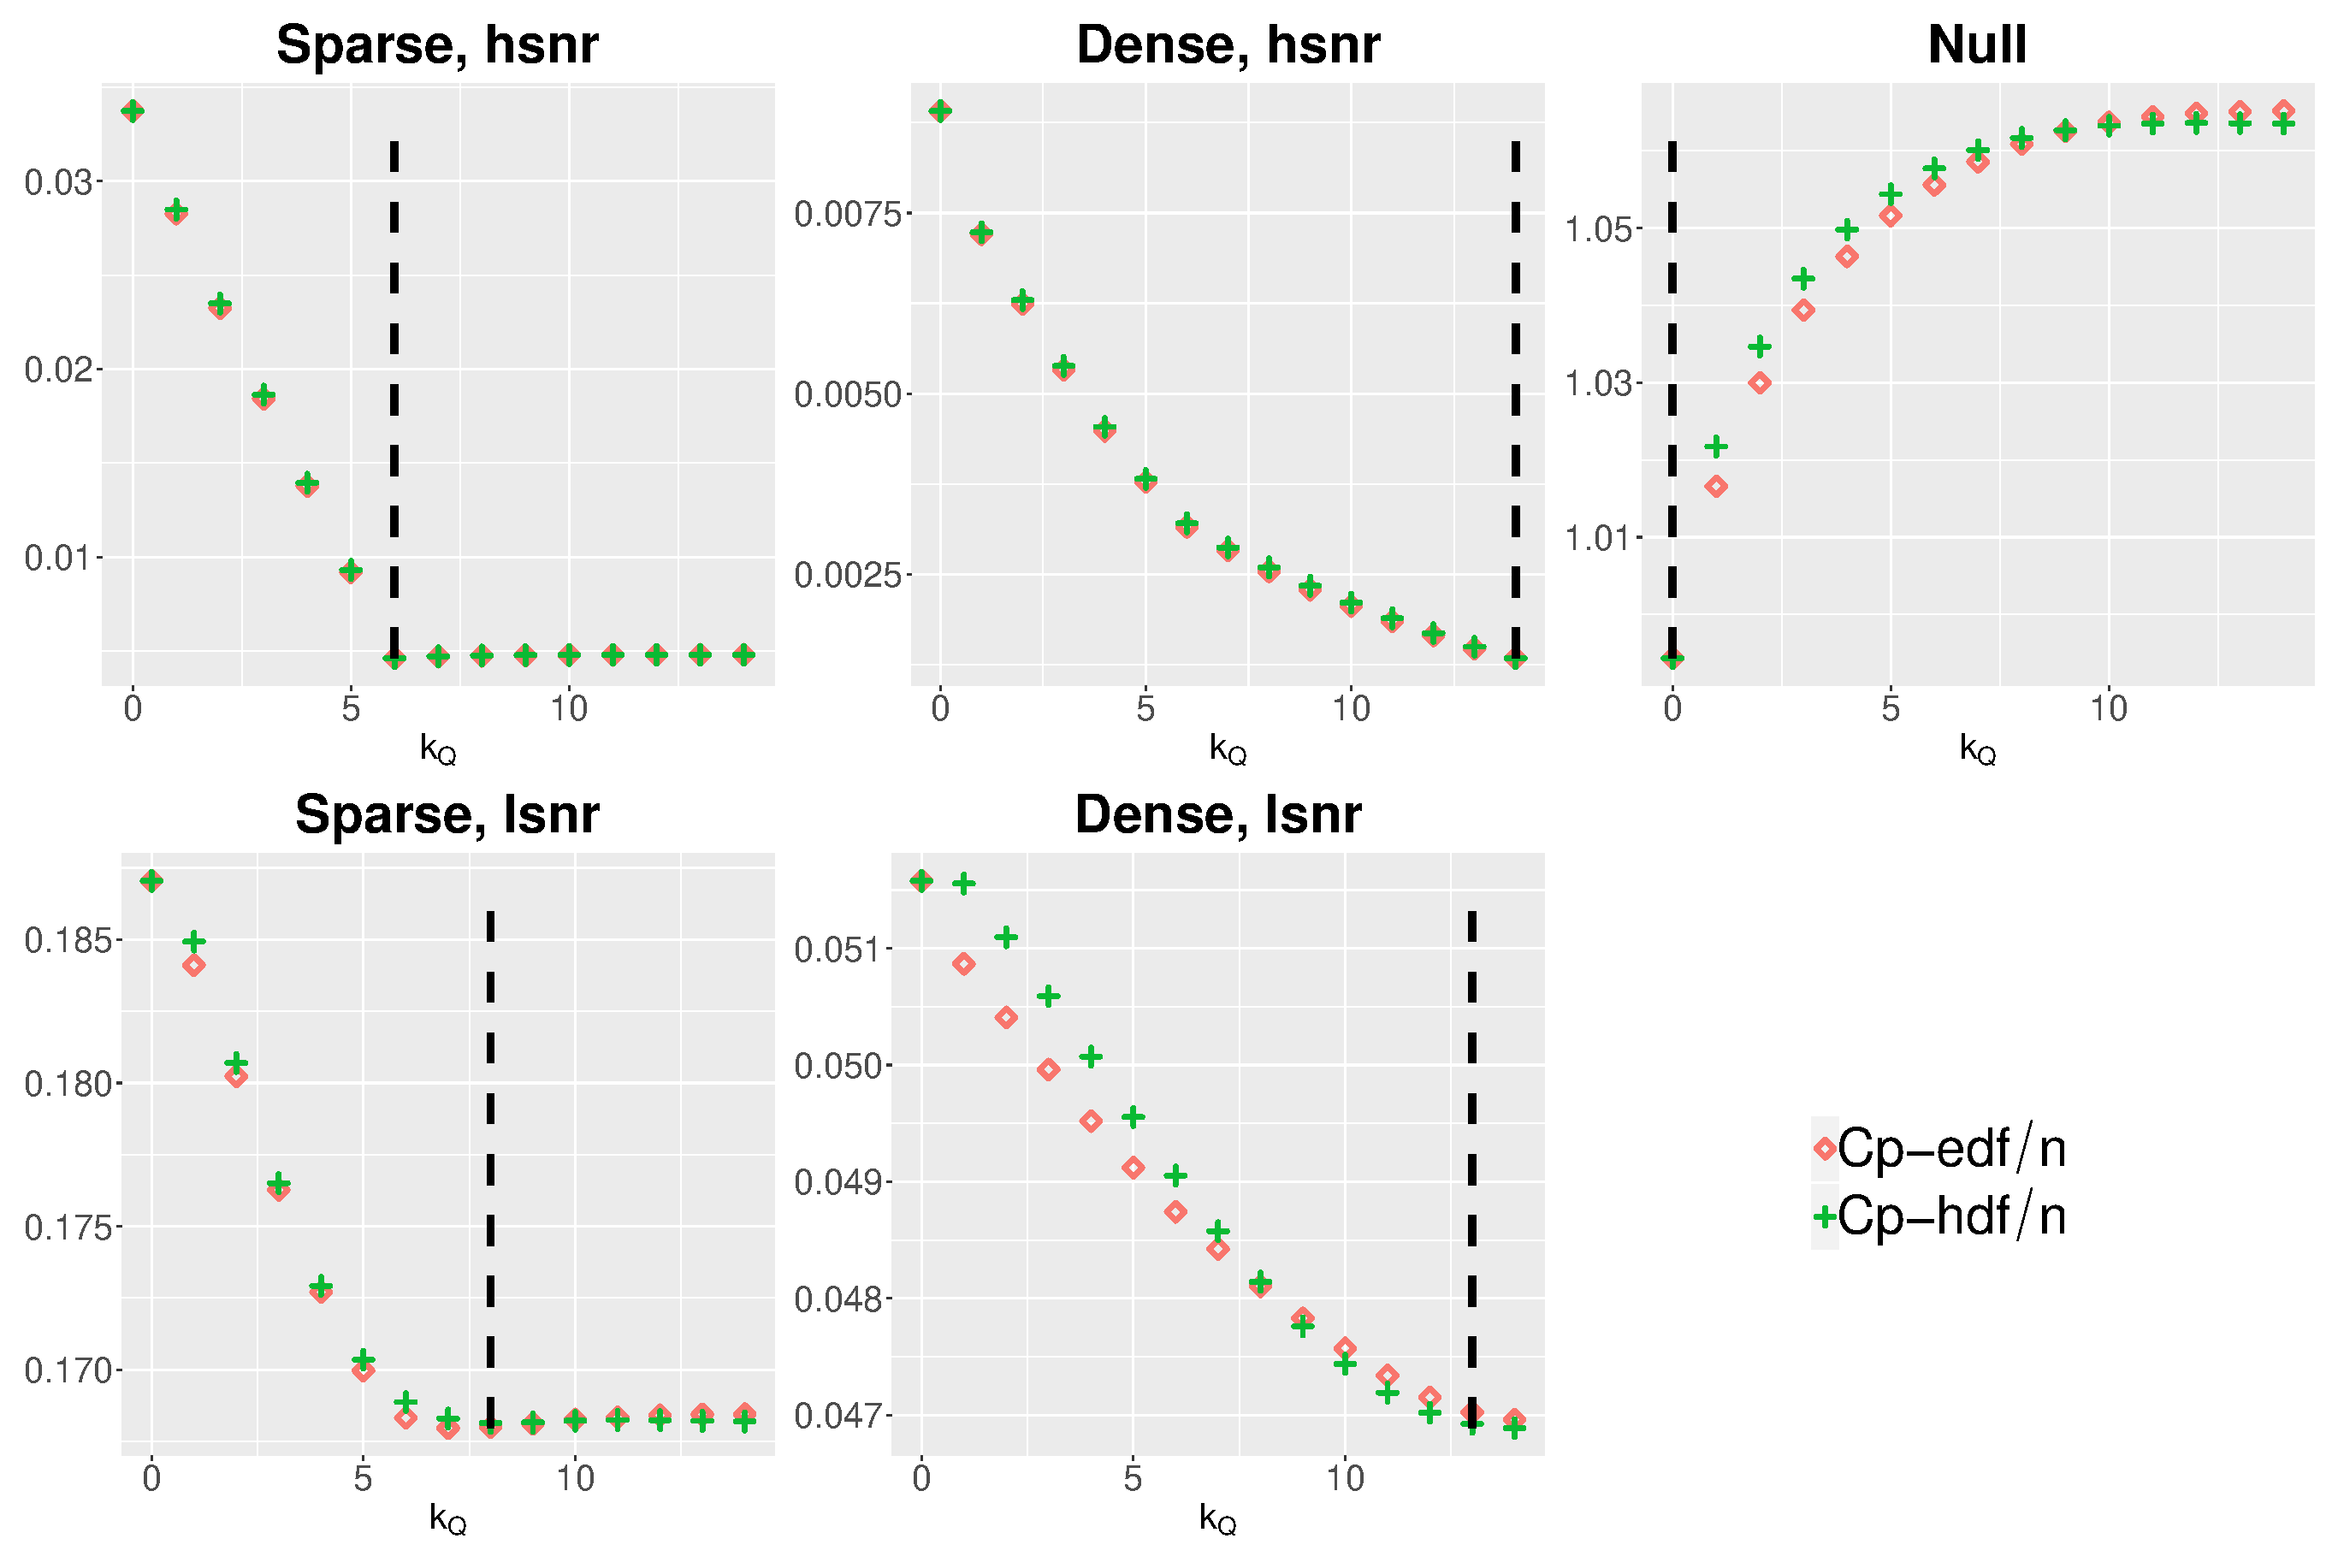
\includegraphics[width=0.9\textwidth]{figures/cp_edf_hdf_boss.eps}
	\caption{Averages of C$_p$-edf and C$_p$-hdf for BOSS over $1000$ replications. Here $X$ is general with $n=200$, $p=14$. Both criteria result in the same average of the selected subset size over the $1000$ replications (rounded to the nearest integer) as denoted by the dashed vertical lines. We assume knowledge of $\mu$ and $\sigma$.}
	\label{fig:boss_cp_edf_hdf}
\end{figure}


% {tab:lbs_bs}
% latex table generated in R 3.6.1 by xtable 1.8-4 package
% Sun Nov 10 00:24:03 2019
\begin{table}[ht]
\centering
\caption{The performance of BS and LBS. The selection rule for both methods is C$_p$-edf. We assume knowledge of $\mu$ and $\sigma$.} 
\label{tab:lbs_bs}
\scalebox{0.9}{
\begin{tabular}{|c|c|c|cc|cc|cc|}
  \toprule 
 \multicolumn{1}{|c}{} & \multicolumn{1}{c}{} &       & \multicolumn{2}{c|}{Orth-Sparse-Ex1} & \multicolumn{2}{c|}{Orth-Sparse-Ex2} & \multicolumn{2}{c|}{Orth-Dense} \\
 \cmidrule{4-9}\multicolumn{1}{|c}{} & \multicolumn{1}{c}{} &       & BS    & LBS   & BS    & LBS   & BS    & LBS  \\
 \midrule 
 \multicolumn{1}{|c}{} & \multicolumn{1}{c}{} &       & \multicolumn{6}{c|}{\% worse than the best possible BS} \\
 \midrule 
 \multirow{4}[4]{*}{n=200} & \multirow{2}[2]{*}{hsnr} & p=30 & 4 & 28 & 21 & 25 & 1 & 1 \\ 
   &  & p=180 & 1 & 43 & 12 & 25 & 7 & 10 \\ 
  \cmidrule{2-9} & \multirow{2}[2]{*}{lsnr} & p=30 & 20 & 26 & 21 & 30 & 15 & 16 \\ 
   &  & p=180 & 15 & 20 & 15 & 32 & 8 & 12 \\ 
  \midrule \multirow{4}[4]{*}{n=2000} & \multirow{2}[2]{*}{hsnr} & p=30 & 3 & 29 & 3 & 28 & 0 & 0 \\ 
   &  & p=180 & 0 & 42 & 0 & 41 & 6 & 9 \\ 
  \cmidrule{2-9} & \multirow{2}[2]{*}{lsnr} & p=30 & 3 & 28 & 7 & 25 & 2 & 2 \\ 
   &  & p=180 & 0 & 41 & 1 & 37 & 8 & 12 \\ 
   \midrule 
 \multicolumn{1}{|c}{} & \multicolumn{1}{c}{} &       & \multicolumn{6}{c|}{Relative efficiency} \\
 \midrule 
\multirow{4}[4]{*}{n=200} & \multirow{2}[2]{*}{hsnr} & p=30 & 1 & 0.81 & 1 & 0.96 & 1 & 1 \\ 
   &  & p=180 & 1 & 0.71 & 1 & 0.89 & 1 & 0.97 \\ 
  \cmidrule{2-9} & \multirow{2}[2]{*}{lsnr} & p=30 & 1 & 0.96 & 1 & 0.93 & 0.95 & 0.94 \\ 
   &  & p=180 & 1 & 0.96 & 1 & 0.87 & 1 & 0.95 \\ 
  \midrule \multirow{4}[4]{*}{n=2000} & \multirow{2}[2]{*}{hsnr} & p=30 & 1 & 0.8 & 1 & 0.81 & 1 & 1 \\ 
   &  & p=180 & 1 & 0.71 & 1 & 0.71 & 1 & 0.98 \\ 
  \cmidrule{2-9} & \multirow{2}[2]{*}{lsnr} & p=30 & 1 & 0.81 & 1 & 0.86 & 1 & 1 \\ 
   &  & p=180 & 1 & 0.71 & 1 & 0.74 & 1 & 0.97 \\ 
   \midrule 
 \multicolumn{1}{|c}{} & \multicolumn{1}{c}{} &       & \multicolumn{6}{c|}{Sparsistency (number of extra variables)} \\
 \midrule 
\multirow{4}[4]{*}{n=200} & \multirow{2}[2]{*}{hsnr} & p=30 & 6(0.1) & 6(0.7) & 4.8(0.4) & 5(0.9) & 30 & 29.9 \\ 
   &  & p=180 & 6(0) & 6(0.9) & 4.2(0) & 4.6(0.9) & 20.5 & 21.9 \\ 
  \cmidrule{2-9} & \multirow{2}[2]{*}{lsnr} & p=30 & 4.5(1.9) & 4.4(2.3) & 2.7(0.6) & 2.9(1.1) & 12.8 & 7.6 \\ 
   &  & p=180 & 1.9(0.5) & 2.3(1.4) & 1.9(0.3) & 2.2(1.2) & 0.8 & 2.7 \\ 
  \midrule \multirow{4}[4]{*}{n=2000} & \multirow{2}[2]{*}{hsnr} & p=30 & 6(0.1) & 6(0.7) & 6(0.1) & 6(0.7) & 30 & 30 \\ 
   &  & p=180 & 6(0) & 6(0.8) & 6(0) & 6(0.8) & 32.1 & 34.1 \\ 
  \cmidrule{2-9} & \multirow{2}[2]{*}{lsnr} & p=30 & 6(0.1) & 6(0.7) & 4.1(0.2) & 4.3(0.7) & 28.8 & 29.4 \\ 
   &  & p=180 & 6(0) & 6(0.8) & 4(0) & 4.1(0.8) & 13.9 & 15.9 \\ 
   \bottomrule 
\end{tabular}
}
\end{table}


\clearpage
\begin{figure}[!ht]
	\centering
	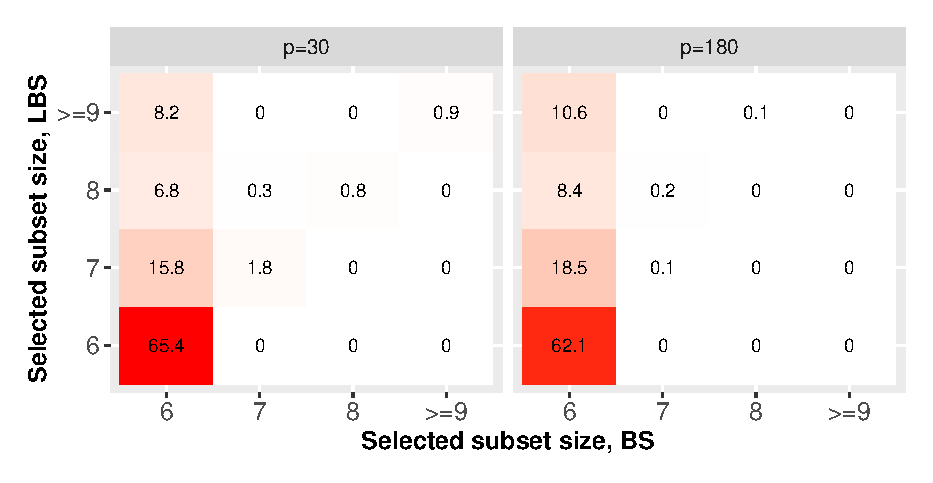
\includegraphics[width=0.9\textwidth]{figures/numvar_bs_lbs.eps}
	\caption{Frequency distributions (in $\%$) of the selected subset size  given by BS and LBS, based on $1000$ replications. The selection rule is C$_p$-edf. The true model is Orth-Sparse-Ex1 with $n=200$, $p_0=6$ and high SNR.}
	\label{fig:numvar_bs_lbs} 
\end{figure}


\iffalse
\begin{figure}[!ht]
	\centering
	\includegraphics[width=0.8\textwidth]{figures/lbs_bs_cp_eg.eps}
	\caption{C$_p$-edf at subset size $k$ for BS and LBS. The true model is Orth-Sparse-Ex1 with $n=200$, $p=180$, $p_0=6$ and high SNR. We assume knowledge of $\mu$ and $\sigma$.}
	\label{fig:lbs_bs_cp_eg} 
\end{figure}
\fi


\clearpage
\bibliographystyleonline{chicago}
\bibliographyonline{reference.bib}
\end{document}
